\documentclass[11pt,a4paper,oldfontcommands]{memoir}
\usepackage{ctex}
\usepackage[utf8]{inputenc}
\usepackage[T1]{fontenc}
\usepackage{microtype}
\usepackage[dvips]{graphicx}
\usepackage{xcolor}
\definecolor{linkColor}{RGB}{0, 153, 230}

\usepackage{times}
\usepackage{listings}
\usepackage{courier}
\lstset{
    columns=fixed,       
    numbers=left,                                        % 在左侧显示行号
    frame=none,                                          % 不显示背景边框
    backgroundcolor=\color[RGB]{245,245,244},            % 设定背景颜色
    keywordstyle=\color[RGB]{40,40,255},                 % 设定关键字颜色
    numberstyle=\footnotesize\color{darkgray},           % 设定行号格式
    commentstyle=\color[RGB]{0,96,96},                   % 设置代码注释的格式
    stringstyle=\rmfamily\slshape\color[RGB]{128,0,0},   % 设置字符串格式
    showstringspaces=false,                              % 不显示字符串中的空格
    language=c++,                                        % 设置语言
    basicstyle=\small\ttfamily
}

\usepackage[
breaklinks=true,colorlinks=true,
%linkcolor=blue,urlcolor=blue,citecolor=blue,% PDF VIEW
linkcolor=black,urlcolor=black,citecolor=black,% PRINT
bookmarks=true,bookmarksopenlevel=2]{hyperref}

\usepackage{amsmath}
\usepackage{hyperref}

\usepackage{geometry}
% PDF VIEW
% \geometry{total={210mm,297mm},
% left=25mm,right=25mm,%
% bindingoffset=0mm, top=25mm,bottom=25mm}
% PRINT
\geometry{total={210mm,297mm},
left=20mm,right=20mm,
bindingoffset=10mm, top=25mm,bottom=25mm}

\OnehalfSpacing
\chapterstyle{bianchi}
\setsecheadstyle{\Large\bfseries\sffamily\raggedright}
\setsubsecheadstyle{\large\bfseries\sffamily\raggedright}
\setsubsubsecheadstyle{\bfseries\sffamily\raggedright}

\pagestyle{plain}
\makepagestyle{plain}
\makeevenfoot{plain}{\thepage}{}{}
\makeoddfoot{plain}{}{}{\thepage}
\makeevenhead{plain}{}{}{}
\makeoddhead{plain}{}{}{}
\maxsecnumdepth{subsection} % chapters, sections, and subsections are numbered
\maxtocdepth{subsection} % chapters, sections, and subsections are in the Table of Contents

\graphicspath{ {./figure/} }

\begin{document}
\thispagestyle{empty}
{
\sffamily
\centering
{\LARGE
Introduction To 3D Game Programming with DirectX12 笔记
}

\vspace{3.5cm}
(草稿)\\
翻译参考\\
\href{http://shiba.hpe.sh.cn/jiaoyanzu/WULI/Soft/NotXNA}{\textcolor{linkColor}{DirecX11 学习笔记}}\\
Google 翻译
\clearpage
\tableofcontents*
\clearpage
\chapter{向量代数(Vector Algebra)}
\chapter{矩阵代数(Matrix Algebra)}
\chapter{矩阵变换(Transformation)}
\chapter{Direct3D 初始化(Direct3D Initialization)}
\section{准备(Preliminaries)}
\subsection{Direct3D 12 概览(Direct3D 12 Overview)}
\subsection{COM}
\subsection{纹理格式(Textures Formats)}
\subsection{交换链与翻页(The Swap Chain and Page Flipping)}
\subsection{深度缓冲(Depth buffering)}
\subsection{资源与描述符(Resources and Descriptors)}
\subsection{多重采样理论(Multisampling Theory)}

\section{CPU/GPU 相互作用(CPU/GPU Interaction)}
\subsection{命令队列和命令列表(The Command Queue and Command Lists)}
\subsection{CPU/GPU 同步(CPU/GPU synchronization)}
\subsection{资源过渡(Resource Transitions)}
\begin{flushleft}
由于有两个并行运行的处理器,出现了许多同步问题。\\
假设我们有一些资源R存储我们想绘制的几何几何的位置。 此外,假设CPU更新R的数据以存储位置p1,然后将引用R的绘图命令C添加到命令队列中,以便在位置p1处绘制几何图形。 将命令添加到命令队列不会阻塞CPU,因此CPU将继续运行。 在GPU执行绘图命令C之前(如图4.7),CPU继续并覆盖R的数据以存储新位置p2将会是错误的。
\end{flushleft}
TODO
\subsection{资源转换(Resource Transitions)}
\begin{flushleft}
为了实现常见的渲染效果,GPU通常在一步中写入资源R,然后在后面的步骤中从资源R中读取。但是,从资源读取资源会造成资源危险。 GPU尚未完成写入或未开始写入。为了解决这个问题,Direct3D将一个状态关联到资源。资源在创建时处于默认状态,并由应用程序告知Direct3D任何状态转换。这使GPU可以做任何需要做的工作来完成转换并防止资源危害。例如,如果我们正在写入资源,比如说纹理,我们会将纹理状态设置为渲染目标状态;当我们需要读取纹理时,我们会将其状态更改为着色器资源状态。通过向Direct3D通知转换,GPU可以采取措施避免危害,例如,在从资源读取之前等待所有写入操作完成。出于性能原因,资源转移的负担落在应用程序开发人员身上。应用程序开发人员知道这些转换何时发生。自动转换跟踪系统会带来额外的开销。\\
通过在命令列表上设置转换资源障碍数组来指定资源转换; 它是一个数组,以防您想要通过一次API调用转换多个资源。 在代码中,资源屏障由D3D12\_RESOURCE\_BARRIER_DESC结构表示。 以下辅助函数(在d3dx12.h中定义)返回给定资源的转换资源屏障描述,并指定之前和之后的状态:\\
\begin{lstlisting}
struct CD3DX12_RESOURCE_BARRIER : public D3D12_RESOURCE_BARRIER
{
    // […] convenience methods
    static inline CD3DX12_RESOURCE_BARRIER Transition(
        _In_ ID3D12Resource* pResource,
        D3D12_RESOURCE_STATES stateBefore,
        D3D12_RESOURCE_STATES stateAfter,
        UINT subresource = D3D12_RESOURCE_BARRIER_ALL_SUBRESOURCES,
        D3D12_RESOURCE_BARRIER_FLAGS flags = D3D12_RESOURCE_BARRIER_FLAG_NONE)
    {
        CD3DX12_RESOURCE_BARRIER result;
        ZeroMemory(&result, sizeof(result));
        D3D12_RESOURCE_BARRIER &barrier = result;
        result.Type = D3D12_RESOURCE_BARRIER_TYPE_TRANSITION;
        result.Flags = flags;
        barrier.Transition.pResource = pResource;
        barrier.Transition.StateBefore = stateBefore;
        barrier.Transition.StateAfter = stateAfter;
        barrier.Transition.Subresource = subresource;
        return result;
    }
    // […] more convenience methods
};
\end{lstlisting}
注意到CD3DX12\_RESOURCE\_BARRIER扩展了D3D12\_RESOURCE\_BARRIER\_DESC并添加了便利方法。 大多数Direct3D 12结构都有助手的变体,我们更喜欢这些变体以方便使用。 CD3DX12的变体全部在d3dx12.h中定义。 该文件不是核心DirectX 12 SDK的一部分,但可以从Microsoft下载。 为方便起见,本书源代码的Common目录中包含一个副本。\\
本章示例应用程序中的一个函数示例如下:\\
\begin{lstlisting}
mCommandList->ResourceBarrier(1,
        &CD3DX12_RESOURCE_BARRIER::Transition(
            CurrentBackBuffer(),
            D3D12_RESOURCE_STATE_PRESENT,
            D3D12_RESOURCE_STATE_RENDER_TARGET));
\end{lstlisting}
此代码将表示我们在屏幕上显示的图像的纹理从呈现状态转换为呈现目标状态。 注意资源屏障已被添加到命令列表中。 您可以将资源屏障转换看作是指示GPU资源状态正在转换的命令,以便在执行后续命令时可以采取必要的步骤来防止资源危险。\\
~\\
NOTICE:除转换类型外,还有其他类型的资源屏障。 目前,我们只需要转换类型。 我们将在需要时介绍其他类型。
\end{flushleft}
\subsection{多线程命令(Multithreading with Commands)}
TODO....

\chapter{渲染管道(The Rendering Pipeline)}
\section{3D图像(The 3D Illusion)}
\section{模型表达(Model Representation)}
\section{基本计算颜色(Basic Computer Color)}
\begin{flushleft}
计算机显示器在每个像素发射一种混合红、绿、蓝三种颜色的光。当这种混合光到达眼睛并且击中视网膜区域,视锥细胞收到刺激并将产生的神经冲动通过视觉神经传递到大脑。大脑解释这种信号为颜色。随着混合光的变化,使这些视锥细胞收到不同的刺激,从而使大脑中产生不同的颜色。\\
\end{flushleft}

\subsection{颜色运算(Color Operations)}
\begin{itemize}
    \item 加法:$(0.0, 0.5, 0) + (0, 0.0, 0.25) = (0.0, 0.5, 0.25)$
    \item 减法:$(1, 1, 1) - (1, 1, 0) = (0, 0, 1)$
    \item 标量乘法:$0.5(1, 1, 1) = (0.5, 0.5, 0.5)$
    \item 显然,点乘和叉乘对于颜色向量来说没有意义。然而,颜色向量有一特殊的运算称为调制或分量乘法:$(c_{r},c_{g},c_{b}) \otimes (k_{r},k_{g},k_{b}) = (c_{r}k_{r},c_{g}k_{g},c_{b}k_{b})$。该运算主要用来作为照明方程。举个例子,假设我们有一束入射光线(r,g,b),它会照射一个反射50%红光,75%绿光和25%蓝光的表面,并吸收剩余的光线。 然后反射光线的颜色由下式给出:$(r,g,b) \otimes (0.5,0.75,0.25) = (0.5r,0.75g,0.25b)$
\end{itemize}

\subsection{128位颜色(128-Bit Color)}
\begin{flushleft}
通常我们会合并另外的颜色分量,称作 alpha 分量。alpha 分量常用来表示颜色的透明度(透明度在混合中很有用,因为我们还没有使用混合,目前只需将 alpha 分量设为 1 即可)。包含 alpha 分量意味着我们用 4D 颜色向量$(r, g, b, a), 0 \leq r,g,b,a \leq 1$ 为了用 128-bits 表示一种颜色,每个分量使用浮点型值。因为数学上,一种颜色就是一个 4D 向量,我们能在代码中使用 XMVECTOR 类型来表示一种颜色,并且每当调用 DirectX Math 中的向量函数时都会受益于 SIMD (如,颜色加减和标量乘法)。为了方便分量乘法,DirectX Math 库提供了下面方法:
\begin{lstlisting}
// Return c1 \otimes c2
XMVECTOR XM_CALLCONV XMColorModulate(FXMVECTOR C1, FXMVECTOR C2);
\end{lstlisting}
\end{flushleft}

\subsection{32位颜色(32-Bit Color)}
\begin{flushleft}
要以32位大小来表示一个颜色,可以给每个分量分配一个字节(8-bit)大小。这样一来,每个分量最多能表现256种色调——0代表无强度,255代表满强度,中间值代表中间强度。看似每个分量一个字节很小,但是组合在一起$(256 \times 256 \times 256)$就表示百万种不同的颜色。DirectX Math 库(\#include <DirectXPackedVector.h>) DirectX::PackedVector 命名空间(namespace)下提供了以下数据结构来存储32位颜色:
\begin{lstlisting}
namespace DirectX
{
namespace PackedVector
{
    // ARGB Color; 8-8-8-8 bit unsigned normalized integer components packed
    // into a 32 bit integer. The normalized color is packed into 32 bits
    // using 8 bit unsigned, normalized integers for the alpha, red, green,
    // and blue components.
    // The alpha component is stored in the most significant bits and the
    // blue component in the least significant bits (A8R8G8B8):
    // [32] aaaaaaaa rrrrrrrr gggggggg bbbbbbbb [0]
    struct XMCOLOR
    {
        union
        {
            struct
            {
                uint8_t b; // Blue: 0/255 to 255/255
                uint8_t g; // Green: 0/255 to 255/255
                uint8_t r; // Red: 0/255 to 255/255
                uint8_t a; // Alpha: 0/255 to 255/255
            };
            uint32_t c;
        };
        XMCOLOR() {}
        XMCOLOR(uint32_t Color) : c(Color) {}
        XMCOLOR(float _r, float _g, float _b, float _a);
        explicit XMCOLOR(_In_reads_(4) const float *pArray);
        operator uint32_t () const { return c; }
        XMCOLOR& operator= (const XMCOLOR& Color) 
        { c = Color.c; return *this; }
        XMCOLOR& operator= (const uint32_t Color) 
        { c = Color; return *this; }
    };
} // end PackedVector namespace
} // end DirectX namespace
\end{lstlisting}
一个32位颜色数据能被转换为128位颜色数据: 将整数区间$[0, 255]$ 映射到实数区间$[0, 1]$。每个数除以255即可,也就是说 设$0 \leq n \leq 255$,且 n 是整数,则 $0 \leq \frac{n}{255} \leq 1$ 就是需要的范围 0 到 1 的颜色强度。例:(80,140,200,255)转换如下:
$$ (80,140,200,255)\rightarrow (\frac{80}{255},\frac{140}{255},\frac{200}{255},\frac{255}{255}) \approx (0.31,0.55,0.78,1.0)$$
另一方面,128位颜色能转换为32位颜色:将每个分量乘以255并且四舍五入取整。例:
$$(0.3,0.6,0.9,1.0)\rightarrow (0.3\cdot 255,0.6\cdot 255,0.9\cdot 255,1.0\cdot 255)=(77,153,230,255)$$

在将32位颜色转换为128位颜色时通常必须执行额外的位操作,反之,因为8位颜色组件通常打包为32位整数值(如 unsigned int),XMCOLOR 就是如此。DirectXMath 库定义了一个方法以 XMCOLOR 作为参数,返回XMVECTOR:
\begin{lstlisting}
XMVECTOR XM_CALLCONV PackedVector::XMLoadColor(const XMCOLOR* pSource);
\end{lstlisting}
\end{flushleft}

\section{渲染管道概览(Overview of the rendering pipeline)}
\section{输入汇编程序阶段(The Input Assembler Stage)}
\subsection{顶点(Vertices)}
\subsection{原始拓扑(Primitive Topology)}
\subsection{指数(Indices)}
\section{顶点着色器阶段(The Vertex Shader Stage)}
\subsection{局部空间和世界空间(Local Space and World Space)}
TODO
\subsection{视图空间(View Space)}
\begin{flushleft}
为了形成场景的二维图像,我们必须在场景中放置一个虚拟相机。 相机指定了观众可以看到的世界的多大的体积,以及我们需要生成多大的世界体积来生成二维图像。让我们将一个局部坐标系统(称为视图空间,眼图空间或相机空间)附加到相机,如图\ref{fig:5-19}所示; 也就是说,摄像机坐落在正视z轴的原点处,x轴指向摄像机的右侧,y轴指向摄像机的上方。 而不是描述相对于世界空间的场景顶点,基于相机坐标系,渲染管线的后面阶段很方便地描述它们。从世界空间到视图空间的坐标变换称为视图变换,相应的矩阵称为视图矩阵。\\
\begin{figure}[t]
    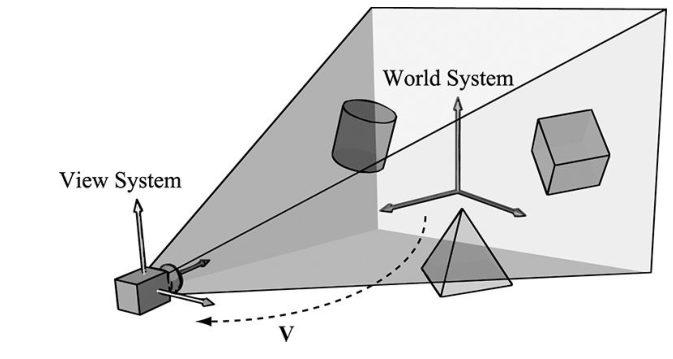
\includegraphics[width=\textwidth]{5-19}
    \centering
    \caption{转换顶点相对于世界空间的坐标,使它们相对于相机空间。}
    \label{fig:5-19}
\end{figure}
如果$Q_{w}=(Q_{x},Q_{y},Q_{z},1)$,$u_{w}=(u_{x},u_{y},u_{z},0)$,$v_{w}=(v_{x},v_{y},v_{z},0)$,$w_{w}=(w_{x},w_{y},w_{z},0)$分别用相对于世界空间的齐次坐标来描述视图空间的原点,x轴,y轴和z轴,然后我们从3.4.3一节知道坐标矩阵从视图空间的变化到世界空间是:
$$W=
\begin{bmatrix}
u_{x} & u_{y} & u_{z} & 0\\
v_{x} & v_{y} & v_{z} & 0\\
w_{x} & w_{y} & w_{z} & 0\\
Q_{x} & Q_{y} & Q_{z} & 1
\end{bmatrix}$$\\
然而,这不是我们想要的转换。我们想要的是倒置转换,即从世界空间转换成视图空间。回忆3.4.3节,倒置转换就是求矩阵的逆。因此$W^{-1}$就是从世界空间到视图空间的转换。\\
世界坐标系统和视图坐标系统仅在位置和方向有区别,所以直观地得到 $W=RT$(也就是说世界矩阵能被分解为一个旋转跟一个平移(translation))\footnote{$R$是\href{https://en.wikipedia.org/wiki/Orthogonal_matrix}{\textcolor{linkColor}{正交矩阵}},所以有 $R^{-1}=R^{T}$}。这让求逆变得简单:
\begin{align*}
V&=W^{-1}=(RT)^{-1}=T^{-1}R^{-1}=T^{-1}R^{T} \\
&=\begin{bmatrix}
1 & 0 & 0 & 0\\
0 & 1 & 0 & 0\\
0 & 0 & 1 & 0\\
-Q_{x} & -Q_{y} & -Q_{z} & 1
\end{bmatrix}
\begin{bmatrix}
u_{x} & v_{x} & w_{x} & 0\\
u_{y} & v_{y} & w_{y} & 0\\
u_{z} & v_{z} & w_{z} & 0\\
0 & 0 & 0 & 0
\end{bmatrix} \\
&=\begin{bmatrix}
u_{x} & v_{x} & w_{x} & 0\\
u_{y} & v_{y} & w_{y} & 0\\
u_{z} & v_{z} & w_{z} & 0\\
\mathbf{-Q\cdot u} & \mathbf{-Q\cdot v} & \mathbf{-Q\cdot w} & 1
\end{bmatrix}
\end{align*}

所以,视图矩阵就是:
\begin{align*}
V=\begin{bmatrix}
u_{x} & v_{x} & w_{x} & 0\\
u_{y} & v_{y} & w_{y} & 0\\
u_{z} & v_{z} & w_{z} & 0\\
\mathbf{-Q\cdot u} & \mathbf{-Q\cdot v} & \mathbf{-Q\cdot w} & 1
\end{bmatrix}
\end{align*}
现在我们用一种直观的方式来构造向量,这些向量用来建立视图矩阵。令\textbf{Q}为摄像机的位置,\textbf{T}为摄像机对准的目标点。然后,令\textbf{j}为世界空间向上方向的单位向量。(本书中,世界坐标系的 xz 构成的平面作为世界地平面,世界 y 轴描述了向上的方向;所以,$j=(0,1,0)$ 就是和世界 y 轴平行的单位向量。然而这只是约定,一些应用可能会选择 xy构成的平面作为地平面,z轴作为向上方向。)参考图片\ref{fig:5-20},摄像机的朝向如下:
$$w=\frac{T-Q}{||T-Q||}$$
该向量描述的是摄像机的z轴,对准\textbf{w}右侧的单位向量:\\
$$u=\frac{j\times w}{||j \times w||}$$
该向量描述的是摄像机的 x 轴。最后,摄像机的y轴单位向量为:\\
$$v=w \times u$$
因为\textbf{w}和\textbf{u}是互相正交的单位向量,$w\times u$也必定是单位向量,没必要正规化。\\
综上所述,给定摄像机的位置,目标点,和世界向上方向,我们就能求得摄像机的本地坐标系统,作为视图矩阵。
\begin{figure}[t]
    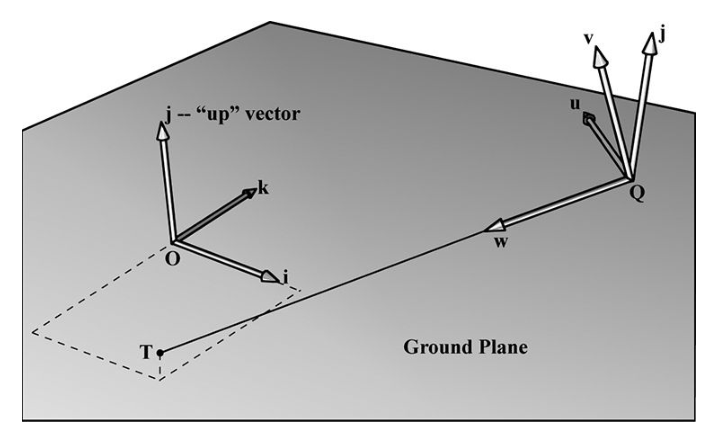
\includegraphics[width=\textwidth]{5-20}
    \centering
    \caption{根据相机位置,目标点和世界“向上”矢量构造相机坐标系。}
    \label{fig:5-20}
\end{figure}

DirectXMath 库提供了计算视图矩阵的方法:
\begin{lstlisting}
// Outputs view matrix V
XMVECTOR XM_CALLCONV XMMatrixLookAtLH(
    FXMVECTOR EyePosition,    // Input camera position Q
    FXMVECTOR FocusPosition,  // Input target point T
    FXMVECTOR UpDirection);   // Input world up direction j
\end{lstlisting}
通常世界y轴就是向上的方向,所以$j=(0,1,0)$ 就是向上的向量。例:假设我们将摄像机放在相对于世界坐标的$(5,3,-10)$处,并且对准世界原点坐标$(0,0,0)$。可以通过下面方式获得视图矩阵:\\
\begin{lstlisting}
XMVECTOR pos    = XMVectorSet(5, 3, -10, 1.0f);
XMVECTOR target = XMVectorZero();
XMVECTOR up     = XMVectorSet(0.0f, 1.0f, 0.0f, 0.0f);
XMMATRIX V      = XMMatrixLookAtLH(pos, target, up);
\end{lstlisting}
\end{flushleft}
\subsection{投影和齐次裁剪空间(Projection and Homogeneous Clip Space)}
\begin{flushleft}
到目前为止我们描述了在世界空间中摄像机的位置和方向,但摄像机还有一个部分需要解决,即摄像机看到的空间体积。体积由视锥来描述(见图\ref{fig:5-21})。
\end{flushleft}
\begin{figure}[t]
    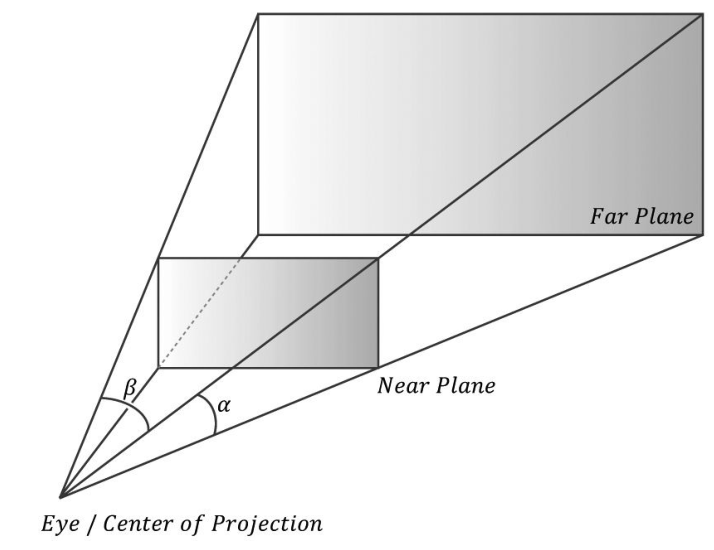
\includegraphics[width=\textwidth]{5-21}
    \centering
    \caption{视锥定义了摄像机“看到”的空间体积}
    \label{fig:5-21}
\end{figure}
\begin{flushleft}
我们接下来的任务是将一个 3D 几何体在视锥中投影到 2D 投影窗口中。投影必须以平行线汇聚到消失点的方式完成,当一个物体的3D深度增加(距离拉远),投影的大小就减小。这就是\href{https://en.wikipedia.org/wiki/Perspective_(graphical)}{\textcolor{linkColor}{透视投影}}(如图\ref{fig:5-22})。我们将一个顶点到视点(眼睛所在的位置,姑且叫视点吧)的连线称为顶点的投影线。然后我们定义透视投影变换就是3D顶点\textbf{v}变换成它的投影线和2D投影面板交叉点\textbf{v'}的过程;我们认为\textbf{v'}就是\textbf{v}的投影。一个3D物体的投影就是组成这个物体的所有顶点的投影。
\end{flushleft}
\begin{figure}[t]
    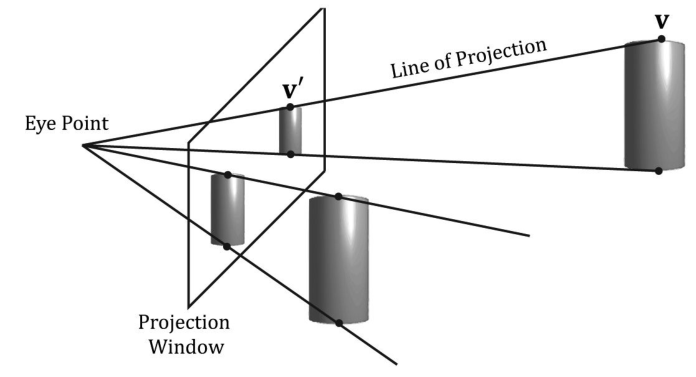
\includegraphics[width=\textwidth]{5-22}
    \centering
    \caption{两个圆柱体大小相同,但深度不同。距离眼睛近的圆柱体比距离远的圆柱体投影大。视锥中的几何体被投影到投影窗口;视锥外的集合体,投影到投影面板上,但在投影窗口外面(投影面板和投影窗口共面)}
    \label{fig:5-22}
\end{figure}

\paragraph{定义一个视锥(Defining a Frustum)}
\begin{flushleft}
我们可以在视图空间中定义一个视锥,其投影中心位于原点处,并沿着正z轴向下看,通过以下四个量:近平面$n$,远平面$f$,垂直视场角$\alpha$ 和纵横比 $r$。请注意,在视图空间中,近平面和远平面平行于$xy$平面; 因此我们只需指定它们沿着z轴的原点距离。 纵横比由 $r=w/h$ 定义,其中$w$是投影窗口的宽度,$h$是投影窗口的高度(视图空间中的单位)。 投影窗口本质上是视图空间中场景的二维图像。 这里的图像最终将映射到后台缓冲区(back buffer); 因此,我们喜欢投影窗口尺寸的比率与后台缓冲区尺寸的比率相同。所以后缓冲区维度的比率通常被指定为长宽比(这是一个比例,所以它没有单位)。例,如果后台缓冲区尺寸是 $800 \times 600$,则 $r=\frac{800}{600} \approx 1.333$。如果投影窗口与后台缓冲区的纵横比不相同,则需要非均匀缩放来将投影窗口映射到后台缓冲区,这将导致失真(例如,投影窗口上的圆圈可能当映射到后台缓冲区时被拉伸成一个椭圆)。\\
我们将水平视角标记为$\beta$,垂直视角标记为$\alpha$,纵横比为$r$。要看看$r$如何帮助我们找到$\beta$,请考虑图\ref{fig:5-23}。 请注意,投影窗口的实际尺寸并不重要,只需要保持纵横比。 因此,我们会选择2的方便高度,因此宽度必须为:\\
$$r=\frac{w}{h}=\frac{w}{2}\Rightarrow w=2r$$
\end{flushleft}
\begin{figure}[t]
    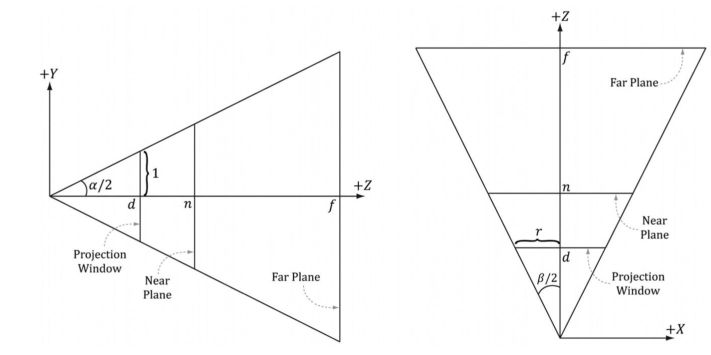
\includegraphics[width=\textwidth]{5-23}
    \centering
    \caption{给定垂直视角$\alpha$和纵横比$r$,得出水平视角$\beta$}
    \label{fig:5-23}
\end{figure}
\begin{flushleft}
为了具有指定的垂直视场$\alpha$,投影窗口必须放置在距离原点的距离$d$处:
$$\tan(\frac{\alpha}{2})=\frac{1}{d}\Rightarrow d=\cot(\frac{\alpha}{2})$$
现在我们已经将投影窗沿$z$轴的距离d固定为当投影窗的高度为2时垂直视场$\alpha$。现在我们可以求解$\beta$。 看一下图\ref{fig:5-23}中的$xz$平面,我们现在看到:
$$\tan(\frac{\beta}{2})=\frac{r}{d}=\frac{r}{\cot(\frac{\alpha}{2})}=r\cdot \tan(\frac{\alpha}{2})$$
因此,考虑到垂直视角α和纵横比r,我们总能得到水平视角β:
$$\beta=2\tan^{-1}(r\cdot\tan(\frac{\alpha}{2}))$$
\end{flushleft}

\paragraph{投影顶点(Projecting Vertices)}
\begin{figure}[t]
    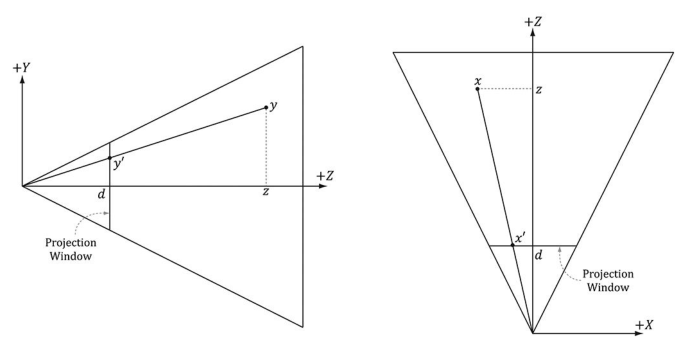
\includegraphics[width=\textwidth]{5-24}
    \centering
    \caption{相似三角}
    \label{fig:5-24}
\end{figure}
\begin{flushleft}
参考图\ref{fig:5-24}。 给定一个点$(x,y,z)$,我们希望在投影平面$z = d$上找到它的投影$(x',y',d)$。 通过分别考虑$x$和$y$坐标并使用相似的三角形,我们发现:
\begin{align*}
\frac{x'}{d}=\frac{x}{z}\Rightarrow x'=\frac{xd}{z}=\frac{x\cot(\alpha/2)}{z}=\frac{x}{z\tan(\alpha/2)}\\
\frac{y'}{d}=\frac{y}{z}\Rightarrow y'=\frac{yd}{z}=\frac{y\cot(\alpha/2)}{z}=\frac{y}{z\tan(\alpha/2)}\\
\end{align*}
显然对于点$(x,y,z)$, $-r\leq x'\leq r,-1\leq y'\leq 1,n\leq z\leq f$
\end{flushleft}

\paragraph{标准化的设备坐标(Normalized Device Coordinate-NDC)}
\begin{flushleft}
上一节中投影点的坐标是在视图空间中计算的。 在视图空间中,投影窗口的高度为2,宽度为$2r$,其中$r$是纵横比。 问题在于,尺寸取决于宽高比。 这意味着我们需要告诉硬件高宽比,因为硬件稍后需要做一些涉及投影窗口尺寸的操作(比如将其映射到后台缓冲区)。 如果我们能够消除这种对长宽比的依赖性会更方便。 解决的办法是将投影的$x$坐标从区间$[-r,r]$缩放到$[-1,1]$像这样:
\begin{align*}
-r\leq x' \leq r \\
-1\leq x'/r \leq 1
\end{align*}

在映射之后,$x$坐标和$y$坐标被称为标准化的设备坐标(NDC)(z坐标还没有被标准化),并且点$(x,y,z)$在视锥内当且仅当:
\begin{align*}
-1\leq x'/r \leq 1 \\
-1\leq y' \leq 1 \\
n \leq z \leq f
\end{align*}

从视图空间到NDC空间的转换可视为单位转换。 我们有一个关系,即一个NDC单位在$x$轴上等于视图空间中的$r$个单位(即 1ndc = \textbf{r} vs)。 所以给定$x$个视图空间单位,我们可以使用这个关系来转换单位:
$$x\mathit{vs}\cdot \frac{1\mathit{ndc}}{r\mathit{vs}}=\frac{x}{r}\mathit{ndc}$$
我们可以修改我们的投影公式,直接在NDC坐标中为我们提供投影的$x$坐标和$y$坐标:
\begin{align*}\tag{eq.5.1}\label{eq.5.1}
x'&=\frac{x}{rz\tan(\alpha/2)}\\
y'&=\frac{y}{z\tan(\alpha/2)}
\end{align*}
请注意,在NDC坐标中,投影窗口的高度为2,宽度为2.因此,现在尺寸是固定的,硬件无需知道纵横比,但我们有责任始终在NDC中提供投影坐标空间(图形硬件假设我们会)。
\end{flushleft}

\paragraph{用矩阵来描述投影公式(Writing the Projection Equations with a Matrix)}
\begin{flushleft}
为了保持一致,我们将用一个矩阵来描述投影变换。不过,公式\ref{eq.5.1}是非线性的,无法用矩阵描述。所以我们要使用一种“技巧”将它分为两部分来实现:一个线性部分和一个非线性部分。非线性部分要除以$z$。我们会在下一节讨论“如何规范化$z$坐标”时讲解这一问题;现在读者只需要知道,我们会因为个除法操作而失去原始的z坐标。所以,我们必须在变换之前保存输入的z坐标;我们可以利用齐次坐标来解决一问题,将输入的$z$坐标复制给输出的$w$坐标。在矩阵乘法中,我们要将元素[2][3]设为1、元素[3][3]设为0(从0开始的索引)。我们的投影矩阵大致如下:
\begin{align*}
P=\begin{bmatrix}
\frac{1}{r\tan(\alpha/2)} & 0 & 0 & 0\\
0 & \frac{1}{\tan(\alpha/2)} & 0 & 0\\
0 & 0 & A & 1\\
0 & 0 & B & 0
\end{bmatrix}
\end{align*}
注意矩阵中的常量$A$和$B$(它们将在下一节讨论);这些常量用于把输入的$z$坐标变换到规范化区间。将一个任意点$(x,y,z,1)$与该矩阵相乘,可以得到:
\begin{align*}\tag{eq.5.2}\label{eq.5.2}
[x,y,z,1]\begin{bmatrix}
\frac{1}{r\tan(\alpha/2)} & 0 & 0 & 0\\
0 & \frac{1}{\tan(\alpha/2)} & 0 & 0\\
0 & 0 & A & 1\\
0 & 0 & B & 0
\end{bmatrix}=\left[ \frac{x}{r\tan(\alpha/2)},\frac{y}{\tan(\alpha/2)},Az+B,z\right]
\end{align*}
在与投影矩阵(线性部分)相乘之后,我们要将每个坐标除以$w = z$(非线性部分),得到最终的变换结果:
\begin{align*}\tag{eq.5.3}\label{eq.5.3}
\left[ \frac{x}{r\tan(\alpha/2)},\frac{y}{\tan(\alpha/2)},Az+B,z\right]
\xrightarrow[]{\text{除以$w$}}
\left[ \frac{x}{rz\tan(\alpha/2)},\frac{y}{z\tan(\alpha/2)},A+\frac{B}{z},1\right]
\end{align*}
顺便提一句,你可能会问:“如何处理除数为0的情况”;对于一问题我们不必担心,因为近平面总是大于0的,其他的点都会被裁剪掉(参见5.9节)。有时,与$w$相除的过程也称为透视除法(perspective divide)或齐次除法(homogeneous divide)。我们可以看到$x$、$y$的投影坐标与公式\ref{eq.5.1}相同。
\end{flushleft}

\paragraph{规范化深度值}
\begin{flushleft}
你可能认为在投影之后可以丢弃原始的3D $z$坐标,因为所有的投影点已经摆放在2D投影窗口上,形成了我们最终看到的2D图像,不会再使用3D $z$坐标了。其实不然,我们仍然需要为深度缓存算法提供3D深度信息。就如同Direct3D希望我们把$x$、$y$投影坐标映射到一个规范化区间一样,Direct3D也希望我们将深度坐标映射到一个规范化区间$[0,1]$中。所以,我们需要创建一个保序函数(order preserving function)$g(x)$把$[n,f]$区间映射到$[0,1]$区间。由于该函数是保序的,所以当$z_{1},z_{2}∈[n,f]$且$z_{1}<z_{2}$时,必有$g(z_{1})<g(z_{2})$。这样,即使深度值已经被变换过了,相对的深度关系还是会被完好无损地保留下来,我们依然可以在规范化区间中得到正确的深度测试结果,这就是我们要为深度缓存算法做的全部工作。
通过缩放和平移可以实现从$[n ,f]$到$[0,1]$的映射。但是,这种方式无法与我们当前的投影方程整合。我们可以从公式\ref{eq.5.3}中看到经过变换的$z$坐标为:
$$g(z)=A+\frac{B}{z}$$
我们现在需要让$A$和$B$满足以下条件:
\begin{itemize}
    \item 条件1:$g(n)=A+\frac{B}{n}$(近平面映射为0)
    \item 条件2:$g(f)=A+\frac{B}{f}$(远平面映射为1)
\end{itemize}
由条件1得到$B$的结果为:$B=-An$。把它代入条件2,得到$A$的结果为:
\begin{align*}
A+\frac{-An}{f}=1\\
\frac{Af-An}{f}=1\\
Af-An=f\\
A=\frac{f}{f-n}
\end{align*}
所以:
\begin{align*}
g(z)=\frac{f}{f-n}-\frac{nf}{(f-n)z}
\end{align*}
从$g(z)$的曲线图(图\ref{fig:5-25})中可以看出,它会限制增长的幅度(保序)而且是非线性的。从图中我们还可以看到,区间中的大部分取值落在近平面附近。因此,大多数深度值被映射到了一个很窄的取值范围内。这会导致深度缓冲区出现精度问题(由于所能表示的数值范围有限,计算机将无法识别变换后的深度值之间的微小差异)。通常的建议是让近平面和远平面尽可能接近,把深度的精度性问题减小到最低程度。
\end{flushleft}
\begin{figure}[b]
    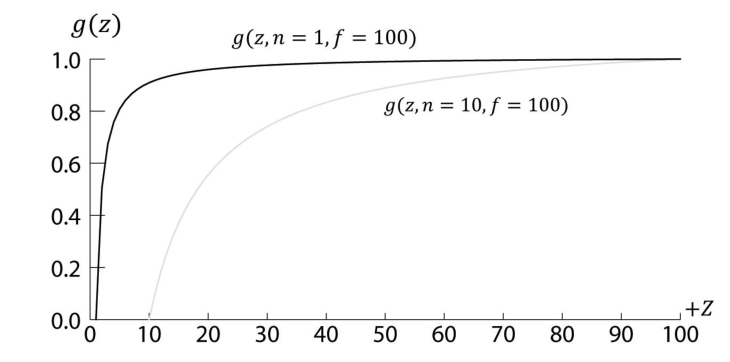
\includegraphics[width=\textwidth]{5-25}
    \centering
    \caption{相对于不同近平面的$g(z)$曲线图}
    \label{fig:5-25}
\end{figure}
\begin{flushleft}
现在我们已经解出了A和B,我们可以确定出完整的透视投影矩阵:
\begin{align*}
P=\begin{bmatrix}
\frac{1}{r\tan(\alpha/2)} & 0 & 0 & 0\\
0 & \frac{1}{\tan(\alpha/2)} & 0 & 0\\
0 & 0 & \frac{f}{f-n} & 1\\
0 & 0 & \frac{-nf}{f-n} & 0
\end{bmatrix}
\end{align*}
在与投影矩阵相乘之后,进行透视除法之前,几何体所处的空间称为齐次裁剪空间(homogeneous clip space)或投影空间(projection space)。在透视除法之后,几何体所处的空间称为规范化设备空间(normalized device coordinates,简称NDC)。
\end{flushleft}

\paragraph{XMMatrixPerspectiveFovLH}
\begin{flushleft}
一个透视投影矩阵能由下面的 DirectX Math 函数生成:
\begin{lstlisting}
// Return the projection matrix
XMMATRIX XM_CALLCONV XMMatrixPerspectiveFovLH(
    float FovAngleY, // vertical field of view angle in radians
    float Aspecct,     // aspect ratio = width / height
    float NearZ,       // distance to near plane
    float FarZ);         // distance to far plane
\end{lstlisting}
下面代码展示了如何使用 XMMatrixPerspectiveFovLH。这里,我们定义垂直视角为$45^{\circ}$,近平面$z=1$,远平面$z=1000$(这些长度都在视图空间)
\begin{lstlisting}
XMMATRIX P= XMMatrixPerspectiveFovLH(0.25f*XM_PI, AspectRatio(),1.0f,1000.0f);
\end{lstlisting}
纵横比匹配窗口的纵横比:
\begin{lstlisting}
float D3DApp::AspectRatio() const
{
  return static_cast<float>(mClientWidth) / mClientHeight;
}
\end{lstlisting}
\end{flushleft}

\section{镶嵌阶段(曲面细分阶段)(The Tessellation Stages)}
\begin{flushleft}
镶嵌(Tessellation)是指通过添加三角形的方式对一个网格的三角形进行细分,这些新添加的三角形可以偏移到一个新的位置,让网格的细节更加丰富。如图\ref{fig:5-26}
\end{flushleft}
\begin{figure}[h]
    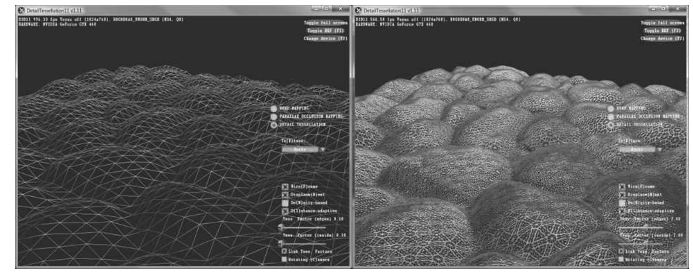
\includegraphics[width=\textwidth]{5-26}
    \centering
    \caption{左图是原网格,右图是镶嵌后的网格}
    \label{fig:5-26}
\end{figure}

\begin{flushleft}
下面是曲面细分的好处:
\begin{itemize}
    \item 我们可以实现细节层次(level-of-detail, LOD),使靠近相机的三角形通过细分产生更多细节,而那些远离相机的三角形则保持不变。通过这种方式,我们只需在需要细节的地方使用更多的三角形就可以了。
    \item 我们可以在内存中保存一个低细节(低细节意味着三角形数量少)的网格,但可以实时地添加额外的三角形,这样可以节省内存。
    \item 我们可以在一个低细节的网格上处理动画和物理效果,而只在渲染时才使用细分过的高细节网格。
\end{itemize}
曲面细分阶段是Direct3D 11中新添加的,这样我们就可以在GPU上对几何体进行细分了。而在Direct3D 11之前,如果你想要实现曲面细分,则必须在CPU上完成,经过细分的几何体还要发送到GPU用于渲染。然而,将新的几何体从CPU内存发送到显存是很慢的,而且还会增加CPU的负担。因此,在Direct3D 11出现之前,曲面细分的方法在实时图形中并不流行。Direct3D 11提供了一个可以完全在硬件上实现的曲面细分API。这样曲面细分就成为了一个非常有吸引力的技术了。曲面细分阶段是可选的(即在需要的时候才使用它)。我们要在第14章才会详细介绍曲面细分。
\end{flushleft}

\section{几何着色阶段(The Geometry Shader Stage)}
\begin{flushleft}
几何着色器阶段(geometry shader stage)是可选的,我们在第12章之前不会用到它,所以这里只做一个简短的概述。几何着色器以完整的图元作为输入数据。例如,当我们绘制三角形列表时,输入到几何着色器的数据是构成三角形的三个点。(注意,这三个点是从顶点着色器传递过来的。)几何着色器的主要优势是它可以创建或销毁几何体。例如,输入图元可以被扩展为一个或多个其他图元,或者几何着色器可以根据某些条件拒绝输出某些图元。这一点与顶点着色器有明显的不同:顶点着色器无法创建顶点,只要输入一个顶点,那么就必须输出一个顶点。几何着色器通常用于将一个点扩展为一个四边形,或者将一条线扩展为一个四边形。\\
~\\
我们可以在图5.11中看到一个“流输出(stream output)”箭头。也就是,几何着色器可以将顶点数据流输出到内存中的一个顶点缓冲区内,这些顶点可以在管线的随后阶段中渲染出来。这是一项高级技术,我们会在后面的章节中对它进行讨论。\\
~\\
NOTICE:顶点位置在离开几何着色器之前,必须被变换到齐次裁剪空间。
\end{flushleft}

\section{裁剪(Clipping)}
\begin{flushleft}
我们必须完全丢弃在平截头体之外的几何体,裁剪与平截头体边界相交的几何体,只留下平截头体内的部分;图 \ref{fig:5-27}以2D形式说明了一概念。
\begin{figure}[h]
    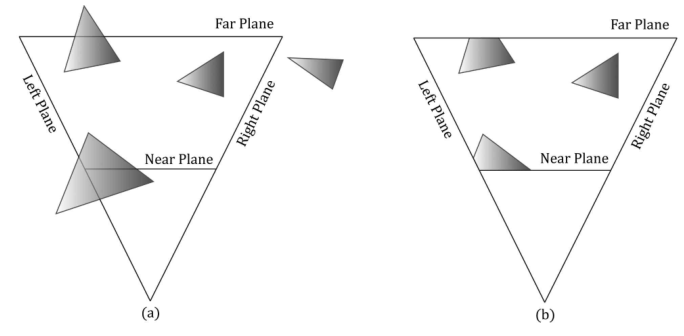
\includegraphics[width=\textwidth]{5-27}
    \centering
    \caption{(a)裁剪之前,(b)裁剪之后}
    \label{fig:5-27}
\end{figure}
我们可以将平截头体视为由6个平面界定的空间范围:顶、底、左、右、近、远平面。要裁剪与平截头体方向相反的多边形,其实就是逐个裁剪与每个平截头体平面方向相反的多边形,当裁剪一个与平面方向相反的多边形时(参见图\ref{fig:5-28}),我们将保留平面正半空间中的部分,而丢弃平面负半空间中的部分。对一个与平面方向相反的凸多边形进行裁剪,得到的结果仍然会是一个凸多边形。由于硬件会自动完成所有的裁剪工作,所以我们不在这里讲解具体的实现细节;有兴趣的读者可以参阅[Sutherland74],了解一下目前流行的Sutherland-Hodgeman裁剪算法。它基本思路是:求出平面与多边形边之间的交点,然后对顶点进行排序,形成新的裁剪后的多边形。\\
\begin{figure}[h]
    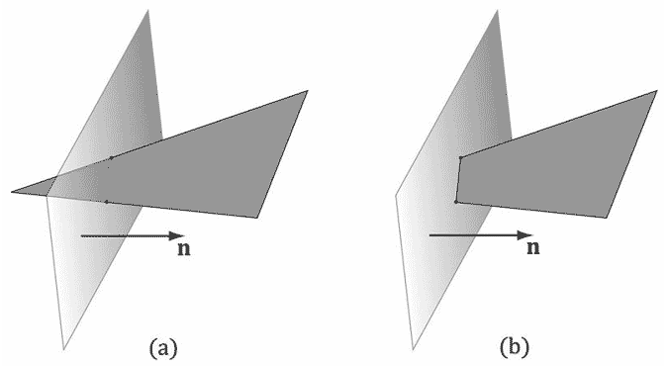
\includegraphics[width=\textwidth]{5-28}
    \centering
    \caption{(a)裁剪一个与平面方向相反的三角形,(b)裁剪后的三角形。注意,裁剪后的三角形已经不再是一个三角形了,它是一个四边形。所以,硬件必须将这个四边形重新划分为三角形,对于凸多边形来说这是一个非常简单的处理过程。}
    \label{fig:5-28}
\end{figure}
\begin{figure}[h]
    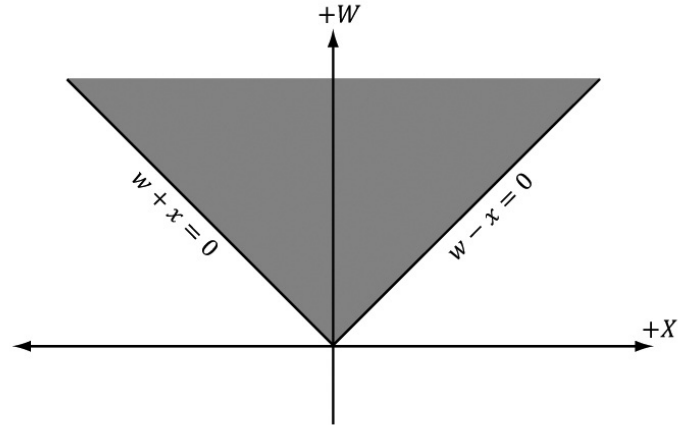
\includegraphics[width=\textwidth]{5-29}
    \centering
    \caption{齐次裁剪空间中$xw$平面上的截头体边界}
    \label{fig:5-29}
\end{figure}
[Blinn78]描述了如何在4D齐次空间中实现裁剪算法(图\ref{fig:5-29})。在透视除法之后,平截头体内的点$ (\frac{x}{w},\frac{y}{w},\frac{z}{w},1) $将位于规范化设备空间,它的边界如下:
\begin{align*}
-1\leq x/w \leq 1\\
-1\leq y/w \leq 1\\
0 \leq z/w \leq 1
\end{align*}
那么在透视除法之前,平截头体内的4D点(x , y , z , w)在齐次裁剪空间中的边界为:
\begin{align*}
-w\leq x \leq w\\
-w\leq y \leq w\\
0 \leq z \leq w
\end{align*}
也就是,顶点被限定在以下4D平面构成的空间范围内:
\begin{align*}
\mathit{Left:}&w=-x\\
\mathit{Right:}&w=x\\
\mathit{Bottom:}&w=-y\\
\mathit{Top:}&w=y\\
\mathit{Near:}&z=0\\
\mathit{Far:}&z=w
\end{align*}
只要我们知道齐次剪裁空间中的平截头体平面方程,我们就能使用任何一种裁剪算法(比如Sutherland-Hodgeman)。注意,由线段/平面相交测试的数学推论可知,这个测试在$\mathbf{R}^{4}$也能使用,所以我们可以在齐次裁剪空间中进行4D点和4D平面的相交测试。
\end{flushleft}

\section{光栅化阶段(The Rasterization Stage)}
\begin{flushleft}
光栅化(rasterization)阶段的主要任务是为投影后的3D三角形计算像素颜色。
\end{flushleft}
\subsection{视口变换(Viewport Transform)}
\begin{flushleft}
在裁剪之后,硬件会自动执行透视除法,将顶点从齐次裁剪空间变换到规范化设备空间(NDC)。一旦顶点进入NDC空间,构成2D图像的2D x、y坐标就会被变换到后台缓冲区中的一个称为视口的矩形区域内(回顾4.2.8节)。在该变换之后,$x$、$y$坐标将以像素为单位。通常,视口变换不修改$z$坐标,因为z坐标还要由深度缓存使用,但是我们可以通过 D3D12\_VIEWPORT 结构体的 MinDepth 和 MaxDepth 值修改z坐标的取值范围。MinDepth 和 MaxDepth 的值必须在0和1之间。
\end{flushleft}
\subsection{背面剔除(Backface Culling)}
\begin{flushleft}
一个三角形有两个面。我们使用如下约定来区分这两个面。假设三角形的顶点按照$v_{0}$、$v_{1}$、$v_{2}$的顺序排列,我们这样来计算三角形的法线$n$:
\begin{align*}
e_{0}&=v_{1}-v_{0}\\
e_{1}&=v_{2}-v_{1}\\
n&=\frac{e_{0}\times e_{1}}{||e_{0}\times e_{1}||}
\end{align*}
带有法线向量的面为正面,而另一个面为背面。图\ref{fig:5-30}说明了这一概念。
\begin{figure}[h]
    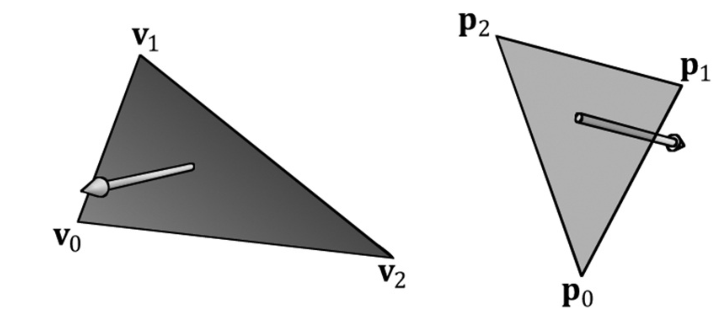
\includegraphics[width=\textwidth]{5-30}
    \centering
    \caption{左边的三角形正对我们的观察点,而右边的三角形背对我们的观察点。}
    \label{fig:5-30}
\end{figure}
当观察者看到三角形的正面时,我们说三角形是朝前的;当观察者看到三角形的背面时, 我们说三角形是朝后的。如图\ref{fig:5-30}所示,左边的三角形是朝前的,而右边的三角形是朝后的。而且,按照我们的观察角度,左边的三角形会按顺时针方向环绕,而右边的三角形会按逆时针方向环绕。这不是巧合:因为按照我们选择的约定(即,我们计算三角形法线的方式),按顺时针方向环绕的三角形(相对于观察者)是朝前的,而按逆时针方向环绕的三角形(相对于观察者)是朝后的。\\
~\\
现在,3D空间中的大部分物体都是封闭实心物体。当我们按照这一方式将每个三角形的法线指向物体外侧时,摄像机就不会看到实心物体朝后的三角形,因为朝前的三角形挡住了朝后的三角形;图\ref{fig:5-31}和图\ref{fig:5-32}分别以2D和3D形式说明了一概念。由于朝前的三角形挡住了朝后的三角形,所以绘制它们是毫无意义的。背面消隐(backface culling)是指让管线放弃对朝后的三角形的处理。这可以将所要处理的三角形的数量降低到原数量的一半。
\end{flushleft}
\begin{figure}[h]
    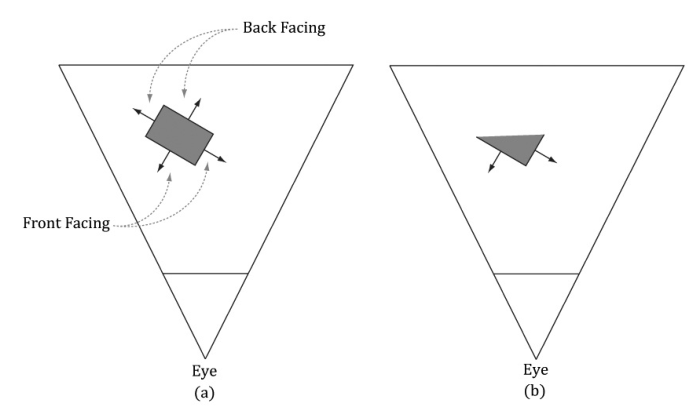
\includegraphics[width=\textwidth]{5-31}
    \centering
    \caption{(a)一个带有朝前和朝后三角形的实心物体。(b)在剔除了朝后的三角形之后的场景。注意,背面消隐不会影响最终的图像,因为朝后的三角形会被朝前的三角形阻挡。}
    \label{fig:5-31}
\end{figure}
\begin{figure}[h]
    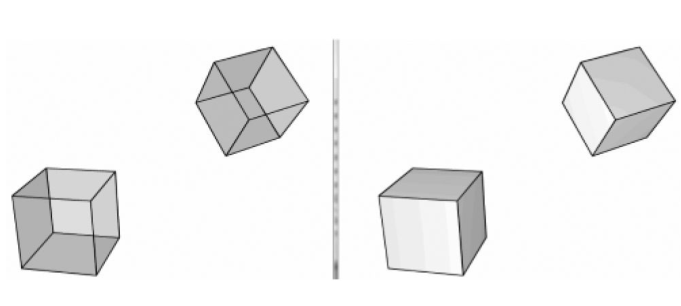
\includegraphics[width=\textwidth]{5-32}
    \centering
    \caption{(左图)当以透明方式绘制立方体时,我们可以看到所有的6个面。(右图)当以实心方式绘制立方体时,我们无法看到朝后的3个面,因为朝前的3个面挡住了它们——所以朝后的三角形可以被直接丢弃,不再接受后续处理,没人能看到些朝后的三角形。}
    \label{fig:5-32}
\end{figure}
\begin{flushleft}
默认情况下,Direct3D将(相对于观察者)顺时针方向环绕的三角形视为朝前的三角形,将(相对于观察者)逆时针方向环绕的三角形视为朝后的三角形。不过,这一约定可以通过修改Direct3D渲染状态颠倒过来。
\end{flushleft}

\subsection{顶点属性插值(Vertex Attribute Interpolation)}
\begin{flushleft}
如前所述,我们通过指定三角形的3个顶点来定义一个三角形。除位置外,顶点还可以包含其他属性,比如颜色、法线向量和纹理坐标。在视口变换之后,这些属性必须为三角形表面上的每个像素进行插值。顶点深度值也必须进行插值,以使每个像素都有一个可用于深度缓存算法的深度值。对屏幕空间中的顶点属性进行插值,其实就是对3D空间中的三角形表面进行线性插值(如图\ref{fig:5-33}所示);这一工作需要借助所谓的透视矫正插值(perspective
correct interpolation)来实现。本质上,三角形表面内部的像素颜色都是通过顶点插值得到的。
\end{flushleft}
\begin{figure}[h]
    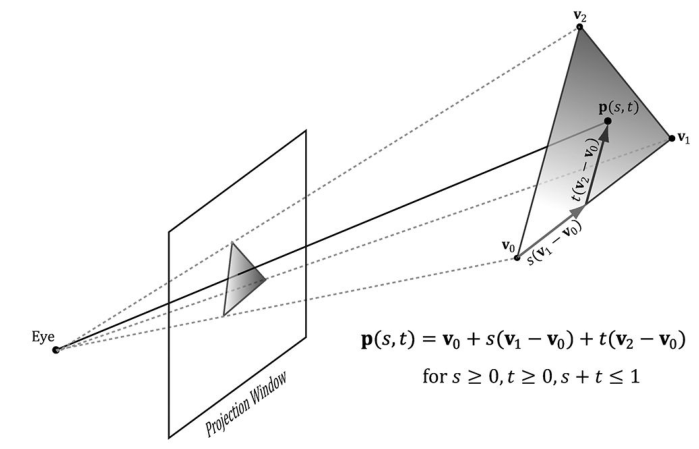
\includegraphics[width=\textwidth]{5-33}
    \centering
    \caption{通过对三角形顶点之间的属性值进行线性插值,可以得到三角形表面上的任一属性值p(s,t)。}
    \label{fig:5-33}
\end{figure}
\begin{flushleft}
我们不必关心透视精确插值的数学细节,因为硬件会自动完成这一工作;不过,有兴趣的读者可以在[Eberly01]中查阅相关的数学推导过程。图5.34介绍了一点基本思路:
\end{flushleft}
\begin{figure}[h]
    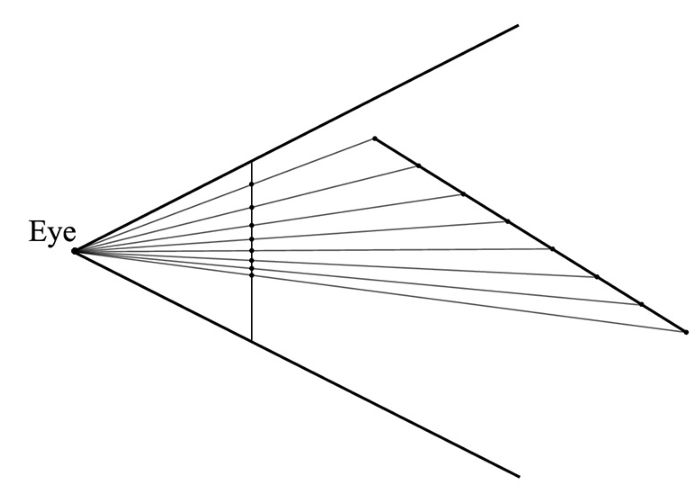
\includegraphics[width=\textwidth]{5-34}
    \centering
    \caption{一条3D线被投影到投影窗口上(在屏幕空间中投影是一条2D线)。我们看到,在3D线上取等距离的点,在2D屏幕空间上的投影点却不是等距离的。所以,我们在3D空间中执行线性插值,在屏幕空间需要执行非线性插值。}
    \label{fig:5-34}
\end{figure}

\section{像素着色器阶段(The Pixel Shader Stage)}
\begin{flushleft}
像素着色器(Pixel shader)是由我们编写的在GPU上执行的程序。像素着色器会处理每个像素片段(pixel fragment),它的输入是插值后的顶点属性,由此计算出一个颜色。像素着色器可以非常简单地输出一个颜色,也可以很复杂,例如实现逐像素光照、反射和阴影等效果。
\end{flushleft}
\section{输出合并阶段(The Output Merger Stage)}
\begin{flushleft}
当像素片段由像素着色器生成之后,它们会被传送到渲染管线的输出合并(output
merger,简称OM)阶段。在该阶段中,某些像素片段会被丢弃(例如,未能通过深度测试或模板测试)。未丢弃的像素片段会被写入后台缓冲区。混合(blending)工作是在该阶段中完成的,一个像素可以与后台缓冲区中的当前像素进行混合,并以混合后的值作为该像素的最终颜色。某些特殊效果,比如透明度,就是通过混合来实现的;我们会在第10章专门讲解混合。
\end{flushleft}

\chapter{在Direct3D中绘制(Drawing in Direct3D)}
\begin{flushleft}
在前一章中,我们主要关注渲染管线的概念和数学方面。 本章反过来关注配置渲染管道,定义顶点和像素着色器以及将几何图形提交到渲染管道进行绘制所需的Direct3D API接口和方法。 到本章结束时,您将能够绘制出具有纯色的3D框或线框模式。\\
~\\
{\large Objectives:}
\begin{itemize}
    \item 发现用于定义,存储和绘制几何数据的Direct3D接口方法。
    \item 学习如何写一个基本顶点和像素着色器
    \item 了解如何用管线状态对象配置渲染管线
    \item 理解如何创建和绑定缓冲数据常量到管线中,并且熟悉根签名
\end{itemize}
\end{flushleft}
\section{定点和顶点布局(Vertices and Input Layouts)}
\begin{flushleft}
5.5.1节已经讲过,在Direct3D中,顶点由空间位置和各种附加属性组成,Direct3D可以让我们灵活地建立属于我们自己的顶点格式;换句话说,它允许我们定义顶点的分量。要创建一个自定义的顶点格式,我们必须先创建一个包含顶点数据的结构体。例如,下面是两种不同类型的顶点格式;一个由位置和颜色组成,另一个由位置、法线和纹理坐标组成。
\end{flushleft}
\begin{lstlisting}
struct Vertex1
{
    XMFLOAT3 Pos;
    XMFLOAT4 Color;
}
struct Vertex2
{
    XMFLOAT3 Pos;
    XMFLOAT3 Normal;
    XMFLOAT2 Tex0;
    XMFLOAT2 Tex1;
}
\end{lstlisting}
\begin{flushleft}
我们定义好顶点构造体后,需要对该定点构造体进行描述然后提供给 Direct3D,让它知道如何去处理每个分量。此描述以D3D12\_INPUT\_LAYOUT\_DESC结构表示的输入布局描述(input layout description)的形式提供给Direct3D:
\begin{lstlisting}
typedef struct D3D12_INPUT_LAYOUT_DESC
{
    const D3D12_INPUT_ELEMENT_DESC *pInputElementDescs;
    UINT NumElements;
} D3D12_INPUT_LAYOUT_DESC;
\end{lstlisting}
一个输入布局描述就是一个简单的 D3D12\_INPUT\_ELEMENT\_DESC 元素数组和元素的数量。\\
~\\
D3D12\_INPUT\_ELEMENT\_DESC数组中的每个元素描述了对应的顶点结构体的分量。如果顶点构造体有两个分量,则对应的 D3D12\_INPUT\_ELEMENT\_DESC数组就有2个元素。D3D12\_INPUT\_ELEMENT\_DESC 定义如下:
\begin{lstlisting}
typedef struct D3D12_INPUT_ELEMENT_DESC
{
    LPCSTR SemanticName;
    UINT SemanticIndex;
    DXGI_FORMAT Format;
    UINT InputSlot;
    UINT AlignedByteOffset;
    D3D12_INPUT_CLASSIFICATION InputSlotClass;
    UINT InstanceDataStepRate;
} D3D12_INPUT_ELEMENT_DESC;
\end{lstlisting}
1. SemanticName: 一个与元素相关的字符串。它可以是任何有效的语义名。语义(semantic)用于将顶点结构体中的元素映射为顶点着色器参数(参见图\ref{fig:6-1})。\\
\begin{figure}[h]
    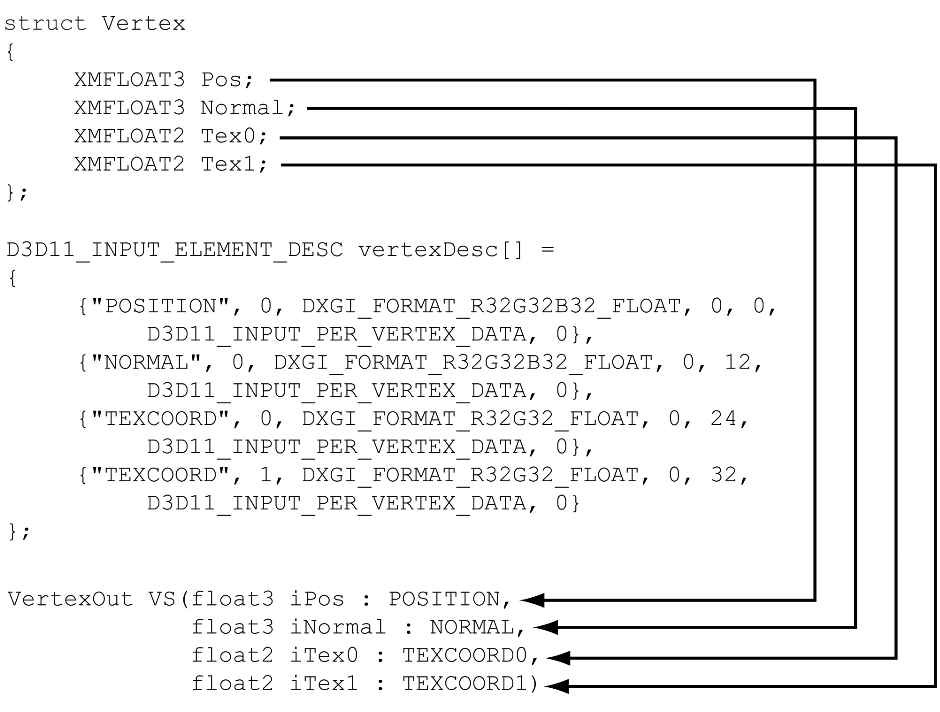
\includegraphics[width=\textwidth]{6-1}
    \centering
    \caption{顶点结构体中的每个元素分别由D3D11\_INPUT\_ELEMENT\_DESC数组中的对应元素描述。语义名和语义索引提供了一种将顶点元素映射为顶点着色器参数的方法。}
    \label{fig:6-1}
\end{figure}
2. SemanticIndex:附加在语义上的索引值。图\ref{fig:6-1}说明了使用该索引的原因;举例来说,当顶点结构体包含多组纹理坐标时,我们不是添加一个新的语义名,而是在语义名的后面加上一个索引值。在着色器代码中没有指定索引的语义默认索引为0,例如,在图\ref{fig:6-1}中的POSITION相当于POSITION0。\\
3. Format:一个用于指定元素格式的DXGI\_FORMAT枚举类型成员;下面是一些常用的格式:
\begin{lstlisting}
DXGI_FORMAT_R32_FLOAT          // 1D 32-bit float scalar
DXGI_FORMAT_R32G32_FLOAT       // 2D 32-bit float vector
DXGI_FORMAT_R32G32B32_FLOAT    // 3D 32-bit float vector
DXGI_FORMAT_R32G32B32A32_FLOAT // 4D 32-bit float vector
DXGI_FORMAT_R8_UINT            // 1D 8-bit unsigned integer scalar
DXGI_FORMAT_R16G16_SINT        // 2D 16-bit signed integer vector
DXGI_FORMAT_R32G32B32_UINT     // 3D 32-bit unsigned integer vector
DXGI_FORMAT_R8G8B8A8_SINT      // 4D 8-bit signed integer vector
DXGI_FORMAT_R8G8B8A8_UINT      // 4D 8-bit unsigned integer vector
\end{lstlisting}
4. InputSlot:指定当前元素来自于哪个输入槽(input slot)。Direct3D支持16个输入槽(索引依次为 0到15),通过这些输入槽我们可以向Direct3D传入顶点数据。例如,当一个顶点由位置元素和颜色元素组成时,我们既可以使用一个输入槽传送两种元素,也可以将两种元素分开,使用第一个输入槽传送顶点元素,使用第二个输入槽传送颜色元素。Direct3D可以将来自于不同输入槽的元素重新组合为顶点。在本书中,我们只使用一个输入槽,但是在本章结尾的练习2中我们会引导读者做一个使用两个输入槽的练习。\\
5. AlignedByteOffset:对于单个输入槽来说,该参数表示从顶点结构体的起始位置到顶点元素的起始位置之间的字节偏移量。例如在下面的顶点结构体中,元素Pos的字节偏移量为0,因为它的起始位置与顶点结构体的起始位置相同;元素Normal的字节偏移量为12,因为必须跳过由Pos占用的字节才能到达Normal的起始位置;元素Tex0的字节偏移量为24,因为必须跳过由Pos和Normal占用的字节才能到达Tex0的起始位置;元素Tex1的字节偏移量为32,因为必须跳过由Pos,Normal和Tex0占用的字节才能到达Tex1的起始位置。\\
\begin{lstlisting}
struct Vertex2
{
    XMFLOAT3 Pos;     // 0-byte offset
    XMFLOAT3 Normal;  // 12-byte offset
    XMFLOAT2 Tex0;    // 24-byte offset
    XMFLOAT2 Tex1;    // 32-byte offset
}
\end{lstlisting}
6. InputSlotClass:目前指定为D3D12\_INPUT\_PER\_VERTEX\_DATA;其他选项用于高级实例技术。\\
7. InstanceDataStepRate:目前指定为0;其他值只用于高级实例技术。\\
~\\
对于前面的两个示例顶点结构体Vertex1和Vertex2来说,对应的输入布局描述为:
\begin{lstlisting}
D3D12_INPUT_ELEMENT_DESC desc1[] = 
{
    {"POSITION", 0, DXGI_FORMAT_R32G32B32_FLOAT, 0, 0, D3D12_INPUT_PRE_VERTEX_DATA, 0},
    {"COLOR", 0, DXGI_FORMAT_R32G32B32A32_FLOAT, 0, 12, D3D12_INPUT_PRE_VERTEX_DATA, 0}
};
D3D12_INPUT_ELEMENT_DESC desc2[] =
{
    {"POSITION", 0, DXGI_FORMAT_R32G32B32_FLOAT, 0, 0,  D3D12_INPUT_PRE_VERTEX_DATA, 0},
    {"NORMAL", 0, DXGI_FORMAT_R32G32B32_FLOAT, 0, 12, D3D12_INPUT_PRE_VERTEX_DATA, 0},
    {"TEXCOORD", 0, DXGI_FORMAT_R32G32_FLOAT, 0, 24, D3D12_INPUT_PRE_VERTEX_DATA, 0},
    {"TEXCOORD", 1, DXGI_FORMAT_R32G32_FLOAT, 0, 32, D3D12_INPUT_PRE_VERTEX_DATA, 0}
};
\end{lstlisting}
\end{flushleft}
\section{顶点缓冲(Vertex Buffers)}
\begin{flushleft}
为了让GPU访问顶点数组,我们必须把它放置在一个称为缓冲(buffer)的GPU资源容器中, 我们称存储顶点的缓冲区叫顶点缓冲区。 缓冲区比纹理资源简单; 它们不是多维的,并且没有mipmap,过滤器或多采样支持。 无论何时我们需要为GPU提供一系列数据元素(如顶点),我们都会使用缓冲区。\\
~\\
就像4.3.8节一样,我们通过填充一个 D3D12\_RESOURCE\_DESC结构体来创建一个 ID3D12Resource 对象,并将其作为缓冲区资源。然后调用 ID3D12Device::CreateCommitedResource 方法。D3D12\_RESOURCE\_DESC 成员详情见 4.3.8 节。Direct3D 12 提供一个 C++ 包装类 CD3DX12\_RESOURCE\_DESC,它是 D3D12\_RESOURCE\_DESC 的衍生类,提供了方便的构造函数和方法。特别是,它提供了以下方法来简化描述缓冲区的D3D12\_RESOURCE\_DESC的构造:
\begin{lstlisting}
static inline CD3DX12_RESOURCE_DESC Buffer(
    UINT64 width, 
    D3D12_RESOURCE_FLAGS flags = D3D12_RESOURCE_FLAG_NONE,
    UINT64 alignment = 0)
{
    return CD3DX12_RESOURCE_DESC(D3D12_RESOURCE_DIMENSION_BUFFER, 
            alignment, width, 1, 1, 1, 
            DXGI_FORMAT_UNKNOWN, 1, 0,
            D3D12_TEXTURE_LAYOUT_ROW_MAJOR, flags);
}
\end{lstlisting}
对于一个缓冲区,width 相当于缓冲区的字节数。例,如果一个缓冲区存储64个浮点型(float),则 width 就是 64*sizeof(float)。\\
~\\
NOTICE: CD3DX12\_RESOURCE\_DESC类还提供了其他针对纹理资源和查询资源的方法:\\
\begin{itemize}
    \item 1. CD3DX12\_RESOURCE\_DESC::Tex1D
    \item 2. CD3DX12\_RESOURCE\_DESC::Tex2D
    \item 3. CD3DX12\_RESOURCE\_DESC::Tex3D
\end{itemize}
~\\
NOTICE:回忆第4章深度/模板缓冲区(depth/stencil buffer),这一阶段用ID3D12Resource 来表现 2D 纹理。所有在 Direct3D 12 的资源都用 ID3D12Resource 接口来表示。着和 Direct3D 11 中使用不同的接口表示不同的资源相反,像 ID3D11Buffer,ID3D11Texture2D。资源类型由 D3D12\_RESOURCE\_DESC::D3D12\_RESOURCE\_DIMENSION 属性指定。例:缓冲区有 D3D12\_RESOURCE\_DIMENSION\_BUFFER 和 2D 纹理 D3D12\_RESOURCE\_DIMENSION\_TEXTURE2D。\\
~\\
对于常量几何(不以每帧为基础改变的几何图形),我们将顶点缓冲区(vertex buffer)放入默认堆(D3D12\_HEAP\_TYPE\_DEFAULT)中,以提升性能。通常,一个游戏中大多数几何图形都是常量集合,像树、建筑、地形、人物等。顶点缓冲区初始化之后,只有GPU需要从顶点缓冲区中读取并画几何图形,所以默认堆就变得有意义了。然而,如果CPU不能将顶点缓冲区写入到默认堆中,我们如何才能初始化顶点缓冲区呢?\\
~\\
另外要新建实际的缓冲区资源,我们需要用D3D12\_HEAP\_TYPE\_UPLOAD新建一个中间上传缓冲资源。回忆4.3.8节,当我们需要从CPU到GPU复制数据时,我们将一个资源提交到上传队中。在创建上传缓冲区之后,从系统内存中复制顶点数据到上传缓冲区,然后从上唇缓冲区复制顶点数据到实际的顶点缓冲区中。\\
~\\
因为一个中间上传缓冲区需要初始化数据后的默认缓冲区(D3D12\_HEAP\_TYPE\_DEFAULT),所以为了代码重用性 d3dUtil.h/cpp 中建立了下面工具方法:
\begin{lstlisting}
Microsoft::WRL::ComPtr<ID3D12Resource> d3dUtil::CreateDefaultBuffer(
    ID3D12Device* device,
    ID3D12GraphicsCommandList* cmdList,
    const void* initData,
    UINT64 byteSize,
    Microsoft::WRL::ComPtr<ID3D12Resource>& uploadBuffer)
{
ComPtr<ID3D12Resource> defaultBuffer;

    // Create the actual default buffer resource.
    ThrowIfFailed(device->CreateCommittedResource(
        &CD3DX12_HEAP_PROPERTIES(D3D12_HEAP_TYPE_DEFAULT),
        D3D12_HEAP_FLAG_NONE,
        &CD3DX12_RESOURCE_DESC::Buffer(byteSize),
        D3D12_RESOURCE_STATE_COMMON,
        nullptr,
        IID_PPV_ARGS(defaultBuffer.GetAddressOf())));

    // In order to copy CPU memory data into our default buffer, we need to create
    // an intermediate upload heap. 
    ThrowIfFailed(device->CreateCommittedResource(
        &CD3DX12_HEAP_PROPERTIES(D3D12_HEAP_TYPE_UPLOAD),
        D3D12_HEAP_FLAG_NONE,
        &CD3DX12_RESOURCE_DESC::Buffer(byteSize),
        D3D12_RESOURCE_STATE_GENERIC_READ,
        nullptr,
        IID_PPV_ARGS(uploadBuffer.GetAddressOf())));

    // Describe the data we want to copy into the default buffer.
    D3D12_SUBRESOURCE_DATA subResourceData = {};
    subResourceData.pData = initData;
    subResourceData.RowPitch = byteSize;
    subResourceData.SlicePitch = subResourceData.RowPitch;

    // Schedule to copy the data to the default buffer resource.  
    // At a high level, the helper function UpdateSubresources
    // will copy the CPU memory into the intermediate upload heap.  
    // Then, using ID3D12CommandList::CopySubresourceRegion,
    // the intermediate upload heap data will be copied to mBuffer.
    cmdList->ResourceBarrier(1, &CD3DX12_RESOURCE_BARRIER::Transition(defaultBuffer.Get(), 
        D3D12_RESOURCE_STATE_COMMON, D3D12_RESOURCE_STATE_COPY_DEST));
    UpdateSubresources<1>(cmdList, defaultBuffer.Get(), uploadBuffer.Get(), 0, 0, 1, &subResourceData);
    cmdList->ResourceBarrier(1, &CD3DX12_RESOURCE_BARRIER::Transition(defaultBuffer.Get(),
        D3D12_RESOURCE_STATE_COPY_DEST, D3D12_RESOURCE_STATE_GENERIC_READ));

    // Note: uploadBuffer has to be kept alive after the above function calls because
    // the command list has not been executed yet that performs the actual copy.
    // The caller can Release the uploadBuffer after it knows the copy has been executed.
    return defaultBuffer;
}
\end{lstlisting}
D3D12\_SUBRESOURCE\_DATA 结构体定义如下:\\
\begin{lstlisting}
typedef struct D3D12_SUBRESOURCE_DATA
{
    const void *pData;
    LONG_PTR RowPitch;
    LONG_PTR SlicePitch;
} D3D12_SUBRESOURCE_DATA;
\end{lstlisting}
1. pData: 指向系统内存数组的指针,该系统内存数组包含了初始化缓冲区所需要的数据。如果缓冲区能保存 n 个顶点,则系统内存数组必须包含至少 n 个顶点的空间,以此来初始化整个缓冲区。\\
2. RowPitch:对于缓冲区,数据复制的字节大小。\\
3. SlicePitch:对于缓冲区,数据复制的字节大小。\\
~\\
下面代码展示了如何该类如何用于创建一个8顶点立方体的默认缓冲区,并且各个定点颜色不同:\\
\begin{lstlisting}
Vertex vertices[] = 
{
    {XMFLOAT3(-1.0f, -1.0f, -1.0f), XMFLOAT4(Colors::White)},
    {XMFLOAT3(-1.0f, +1.0f, -1.0f), XMFLOAT4(Colors::Black)},
    {XMFLOAT3(+1.0f, +1.0f, -1.0f), XMFLOAT4(Colors::Red)},
    {XMFLOAT3(+1.0f, -1.0f, -1.0f), XMFLOAT4(Colors::Green)},
    {XMFLOAT3(-1.0f, -1.0f, +1.0f), XMFLOAT4(Colors::Blue)},
    {XMFLOAT3(-1.0f, +1.0f, +1.0f), XMFLOAT4(Colors::Yellow)},
    {XMFLOAT3(+1.0f, +1.0f, +1.0f), XMFLOAT4(Colors::Cyan)},
    {XMFLOAT3(+1.0f, -1.0f, +1.0f), XMFLOAT4(Colors::Magenta)}
};
const UINT64 vbByteSize = 8 * sizeof(Vertex);
ComPtr<ID3D12Resource> VertexBufferGPU = nullptr;
ComPtr<ID3D12Resource> VertexBufferUploader = nullptr;
VertexBufferGPU = d3dUtil::CreateDefaultBuffer(
    md3dDevice.Get(),
    mCommandList.Get(),
    vertices, vbByteSize,
    VertexBufferUploader);
\end{lstlisting}
Vertex 类型定义如下:\\
\begin{lstlisting}
struct Vertex
{
    XMFLOAT3 Pos;
    XMFLOAT4 Color;
}
\end{lstlisting}
为了将顶点缓冲区绑定到管道,我们需要为顶点缓冲区资源创建一个顶点缓冲区视图(vertex buffer view)。不像一个RTV(render target view),我们不需要一个针对顶点缓冲区视图的描述堆(descriptor heap)。一个顶点缓冲区视图由 D3D12\_VERTEX\_BUFFER\_VIEW\_DESC 结构体表示:\\
\begin{lstlisting}
typedef struct D3D12_VERTEX_BUFFER_VIEW
{
    D3D12_GPU_VIRTUAL_ADDRESS BufferLocation;
    UINT SizeInBytes;
    UINT StrideInBytes;
} D3D12_VERTEX_BUFFER_VIEW;
\end{lstlisting}
1. BufferLocation:创建一个视图所需要的顶点缓冲区资源的虚拟地址。我们可以使用 ID3D12Resource::GetGPUVirtualAddress 方法获得该值。\\
2. SizeInBytes:从BufferLocation开始在顶点缓冲区中查看的字节数。 \\
3. StrideInBytes:每个顶点元素的字节大小。\\
在顶点缓冲区创建之后,我们再创建它的视图,我们能将其绑定到管道(pipeline)的一个输入槽(input slot),给输入汇编程序阶段(input assembler stage)提供顶点数据。使用下面方法就能做到:\\
\begin{lstlisting}
void ID3D12GraphicsCommandList::IASetVertexBuffers(
    UINT StartSlot,
    UINT NumBuffer,
    const D3D12_VERTEX_BUFFER_VIEW *pViews);
\end{lstlisting}
1. StartSlot:绑定顶点缓冲区的开始输入槽。共16个输入槽,0-15。\\
2. NumBuffers:绑定到输入槽的顶点缓冲区个数。如果开始槽索引为k,绑定了 n 个缓冲区,则绑定缓冲区的输入槽分别是$I_{k},I_{k}+1,...,I_{k}+n-1$。\\
3. pViews:指向顶点缓冲区视图数组的第一个元素的指针。\\
调用例子:\\
\begin{lstlisting}
D3D12_VERTEX_BUFFER_VIEW vbv;
vbv.BufferLocation = VertexBufferGPU->GetGPUVirtualAddress();
vbv.StrideInBytes = sizeof(Vertex);
vbv.SizeInBytes = 8 * sizeof(Vertex);
D3D12_VERTEX_BUFFER_VIEW vertexBuffers[1] = {vbv};
mCommandList->IASetVertexBuffers(0, 1, vertexBuffers);
\end{lstlisting}
IASetVertexBuffers 方法可能看起来有点复杂,因为它支持一个顶点缓冲区数组设置到不同的输入槽。然而,我们只使用一个输入槽。本章结尾会有练习,让你使用两个输入槽。\\
一个顶点缓冲区将保持绑定到输入插槽,直到您更改为止。 因此,如果您使用多个顶点缓冲区,则可以像这样构造代码:\\
\begin{lstlisting}
ID3D12Resource* mVB1; // stores vertices of type Vertex1
ID3D12Resource* mVB2; // stores vertices of type Vertex2
D3D12_VERTEX_BUFFER_VIEW_DESC mVBView1; // view to mVB1
D3D12_VERTEX_BUFFER_VIEW_DESC mVBView2; // view to mVB2

/*...Create the vertex buffers and views...*/
mCommandList->IASetVertexBuffers(0, 1, &VBView1);
/*...draw objects using vertex buffer 1...*/

mCommandList->IASetVertexBuffers(0, 1, &mVBView2);
/*...draw objects using vertex buffer 2...*/
\end{lstlisting}
给输入槽设置顶点缓冲区并不意味着绘制它们;这一步只是给管道提供顶点数据。最后一步才是绘制顶点,使用 ID3D12GraphicsCommandList::DrawInstanced 方法:\\
\begin{lstlisting}
void ID3D12GraphicsCommandList::DrawInstanced(
    UINT VertexCountPerInstance,
    UINT InstanceCount,
    UINT StartVertexLocation,
    UINT StartInstanceLocation);
\end{lstlisting}
1. VertexCountPerInstance:绘制顶点的数量(每个实例)。\\
2. InstanceCount:用于称为实例的高级技术; 现在,将其设置为1,因为我们只绘制一个实例。\\
3. StartVertexLocation:指定开始绘制的顶点缓冲区中第一个顶点的索引(从零开始)。\\
4. StartInstanceLocation:用于称为实例的高级技术; 现在,将其设置为0。\\
VertexCountPerInstance和StartVertexLocation这两个参数定义要绘制的顶点缓冲区中的顶点的连续子集;见图\ref{fig:6-2}。\\
\begin{figure}[h]
    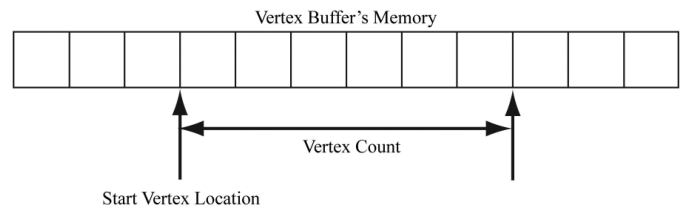
\includegraphics[width=\textwidth]{6-2}
    \centering
    \caption{StartVertexLocation 表示开始绘制的顶点缓冲区的第一个元素。VertexCountPerInstance 表示绘制顶点的个数。}
    \label{fig:6-2}
\end{figure}

DrawInstanced 方法没有制定顶点的基本类型。它们需要被绘制成点,线列表,还是三角列表?回忆5.5.2节,基本拓扑状态是通过 ID3D12GraphicsCommandList::IASetPrimitiveTopology 方法设置的。例:\\
\begin{lstlisting}
mCommandList->IASetPrimitiveTopology(D3D_PRIMITIVE_TOPOLOGY_TRIANGLELIST);
\end{lstlisting}
\end{flushleft}
\section{索引和索引缓冲区(Indices and Index Buffers)}
\begin{flushleft}
与顶点类似,为了让GPU访问索引数组,需要将索引数组放到GPU缓冲区资源中(ID3D12Resource)。我们将存储索引的缓冲区叫索引缓冲区(index buffer)。因为 d3dUtil::CreateDefaultBuffer 方法能通过 void* 作用于一般数据,我们同样使用该方法来创建索引缓冲区(或任何默认缓冲区)。\\
为了将索引缓冲区绑定到管道,我们需要为索引缓冲区资源创建一个索引缓冲区视图。 与顶点缓冲区视图一样,我们不需要一个描述符堆用于索引缓冲区视图。 索引缓冲区视图由D3D12\_INDEX\_BUFFER\_VIEW结构表示:\\
\begin{lstlisting}
typedef struct D3D12_INDEX_BUFFER_VIEW
{
    D3D12_GPU_VIRTUAL_ADDRESS bufferLocation;
    UINT SizeInBytes;
    DXGI_FORMAT Format;
} D3D12_INDEX_BUFFER_VIEW;
\end{lstlisting}
1. BufferLocation: 创建视图的顶点缓冲区资源的虚拟地址。 我们可以使用ID3D12Resource :: GetGPUVirtualAddress方法来获取它。\\
2. SizeInBytes:从BufferLocation开始在索引缓冲区中查看的字节数。\\
3. Format:索引的格式必须是16位索引的 DXGI\_FORMAT\_R16\_UINT 或32位索引的 DXGI\_FORMAT\_R32\_UINT。 如果索引值需要额外的32位范围,则应使用16位索引来减少内存和带宽,并仅使用32位索引。\\
~\\
就顶点缓冲区和其他Direct3D资源而言,在我们可以使用它之前,我们需要将它绑定到管道。 使用 ID3D12CommandList::SetIndexBuffer方法将索引缓冲区绑定到输入汇编程序阶段。 以下代码显示了如何创建一个定义多维数据集三角形的索引缓冲区,创建一个视图并将其绑定到管道:\\
\begin{lstlisting}
std::uint16_t indices[] = {
    // front face
    0, 1, 2,
    0, 2, 3,
    
    // back face
    4, 6, 5,
    4, 7, 6,
    
    // left face
    4, 6, 1,
    4, 1, 0,
    
    // right face
    3, 2, 6,
    3, 6, 7,
    
    // top face
    1, 5, 6,
    1, 6, 2,
    
    // bottom face
    4, 0, 3,
    4, 3, 7
};

const UINT ibByteSize = 36 * sizeof(std::uint16_t);

ComPtr<ID3D12Resource> IndexBufferGPU = nullptr;
ComPtr<ID3D12Resource> IndexBufferUploader = nullptr;
IndexBufferGPU = d3dUtil::CreateDefaultBuffer(md3dDevice.Get(), mCommandList.Get(), indices, ibByteSize, IndexBufferUploader);
D3D12_INDEX_BUFFER_VIEW ibv;
ibv.BufferLocation = IndexBufferGPU->GetGPUVirtualAddress();
ibv.Format = DXGI_FORMAT_R16_UINT;
ibv.SizeInBytes = ibByteSize;

mCommandList->IASetIndexBuffer(&ibv);
\end{lstlisting}
最后,使用索引时,用 ID3D12GraphicsCommandList::DrawIndexedInstanced 方法,而不是 DrawInstanced:\\
\begin{lstlisting}
void ID3D12GraphicsCommandList::DrawIndexedInstanced(
    UINT IndexCountPerInstance,
    UINT InstanceCount,
    UINT StartIndexLocation,
    INT BaseVertexLocation,
    UINT StartInstanceLocation);
\end{lstlisting}
1. IndexCountPerInstance:要绘制的索引数量(每个实例)。\\
2. InstanceCount:用于称为实例的高级技术; 现在,将其设置为1,因为我们只绘制一个实例。\\
3. StartIndexLocation:索引缓冲区中的一个元素索引,标志着开始读取索引的起始点。\\
4. BaseVertexLocation:在获取顶点之前,要将此整数值添加到此绘图调用使用的索引中。\\
5. StartInstanceLocation:用于称为实例的高级技术, 目前指定为0。\\
~\\
为了说明这些参数,请考虑以下情况。假设我们有三个对象:一个球体,一个盒子和一个圆柱体。首先,每个对象都有自己的顶点缓冲区和自己的索引缓冲区。每个本地索引缓冲区中的索引都与相应的本地顶点缓冲区有关。现在假设我们将球体,盒子和圆柱体的顶点和索引连接成一个全局顶点和索引缓冲区,如图\ref{fig:6-3}所示。 (可能会连接顶点和索引缓冲区,因为在更改顶点和索引缓冲区时会有一些API开销,这很可能不是瓶颈,但是如果有许多小的顶点和索引缓冲区可以很容易地合并,值得这样做是出于性能方面的原因。)在这个串联之后,索引不再是正确的,因为它们存储索引位置相对于它们相应的本地顶点缓冲区而不是全局索引位置;因此需要重新计算索引以正确地将索引指向全局顶点缓冲区。原始盒子索引是在假设盒子的顶点贯穿索引的情况下计算出来的 0, 1, ..., numBoxVertices-1\\
但是合并之后,就成为:\\
\begin{lstlisting}
firstBoxVertexPos,
firstBoxVertexPos+1,
...,
firstBoxVertexPos+numBoxVertices-1
\end{lstlisting}
 
\begin{figure}[h]
    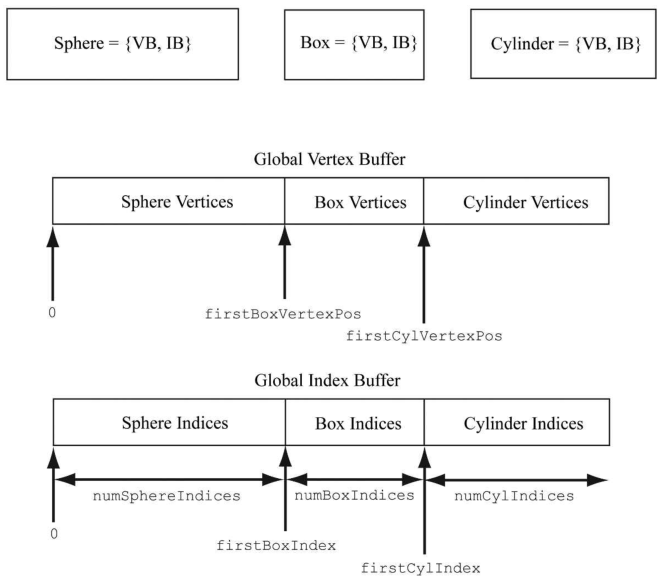
\includegraphics[width=\textwidth]{6-3}
    \centering
    \caption{将几个顶点缓冲区连接成一个大的顶点缓冲区,并将几个索引缓冲区连接成一个大的索引缓冲区。}
    \label{fig:6-3}
\end{figure}

因此,要更新索引,我们需要为每个框索引添加第一个BoxVertexPos。 同样,我们需要为每个柱面索引添加firstCylVertexPos。 请注意,球体的指标不需要改变(因为第一个球体顶点位置为零)。 让我们把对象的第一个顶点相对于全局顶点缓冲区的位置称为它的基本顶点位置。 通常,对象的新索引是通过将其基本顶点位置添加到每个索引来计算的。 我们可以让Direct3D通过将基本顶点位置传递给DrawIndexedInstanced的第四个参数来完成它,而不必自己计算新的索引。\\
然后我们可以用以下三个调用一个接一个地绘制球体,盒子和圆柱体:\\
\begin{lstlisting}
mCmdList->DrawIndexedInstanced(numSphereIndices, 1, 0, 0, 0);
mCmdList->DrawIndexedInstanced(numBoxIndices, 1, firstBoxIndex, firstBoxVertexPos, 0);
mCmdList->DrawIndexedInstanced(numCylIndices, 1, firstCylIndex, firstCylVertexPos, 0);
\end{lstlisting}
下一章(chapter)"Shapse"代码样例就使用了这样的技术。
\end{flushleft}
\section{顶点着色器例子(Example Vertex Shader)}
TODO
\section{像素着色器例子(Example Pixel Shader)}
TODO
\section{常量缓冲区(Constant Buffers)}
\subsection{创建常量缓冲区(Creating Constant Buffers)}
\begin{flushleft}
常量缓冲区是GPU资源(ID3D12Resource)的一个例子,其数据内容可在着色器程序中引用。 正如我们将在本书中学习的那样,着色器程序中也可以引用纹理和其他类型的缓冲区资源。 6.4节中的示例顶点着色器的代码如下:
\begin{lstlisting}
cbuffer cbPerObject: register(b0)
{
    float4x4 gWorldViewProj;
}
\end{lstlisting}
此代码引用一个名为cbPerObject的cbuffer对象(常量缓冲区)。 在这个例子中,常量缓冲区存储一个名为gWorldViewProj的4×4矩阵,表示用于将点从本地空间转换为同类剪辑空间的组合世界,视图和投影矩阵。 在HLSL中,4×4矩阵由内置的float4x4类型声明; 要声明3×4矩阵和2×4矩阵,例如,您将分别使用float3x4和float2x2类型。\\
与顶点和索引缓冲区不同,常量缓冲区通常由CPU每帧更新一次。 例如,如果摄像机每帧移动一次,则每帧必须使用新的视图矩阵更新常量缓冲区。 因此,我们在上传堆而不是默认堆中创建常量缓冲区,以便我们可以从CPU更新内容。\\
常量缓冲区也有特殊的硬件要求,它们的大小必须是最小硬件分配大小(256字节)的倍数。\\
通常我们需要多个相同类型的常量缓冲区。 例如,上面的常量缓冲区cbPerObject存储每个对象不同的常量,所以如果我们有n个对象,那么我们将需要n个这种类型的常量缓冲区。 以下代码显示了我们如何创建一个存储NumElements多个常量缓冲区的缓冲区:
\begin{lstlisting}
struct ObjectConstants
{
    DirectX::XMFLOAT4X4 WorldViewProj = MathHelper::Identity4x4();
};
UINT elementByteSize = d3dUtil::CalcConstantBufferByteSize(sizeof(ObjectConstants));
ComPtr<ID3D12Resource> mUploadCBuffer;
device->CreateCommittedResource(
    &CB3DX12_HEAP_PROPERTIES(D3D12_HEAP_TYPE_UPLOAD), 
    D3D12_HEAP_FLAG_NONE, 
    &CD3DX12_RESOURCE_DESC::Buffer(elementByteSize * NumElements),
    D3D12_RESOURCE_STATE_GENERIC_READ,
    nullptr, 
    IID_PPV_ARGS(&mUploadCBuffer));
\end{lstlisting}
我们可以将mUploadCBuffer视为存储ObjectConstants类型的常量缓冲区数组(使用填充为256的倍数)。 当需要绘制一个对象时,我们只需将一个常量缓冲区视图(CBV)绑定到缓冲区的一个存储该对象常量的子区域。 请注意,我们经常会调用缓冲区mUploadCBuffer作为常量缓冲区,因为它存储了一个常量缓冲区数组。\\
工具函数 d3dUtil::CalcConstantBufferByteSize 会进行算术运算将缓冲区的字节大小舍入为最小硬件分配大小(256字节)的倍数:\\
\begin{lstlisting}
static UINT CalcConstantBufferByteSize(UINT byteSize)
{
    // Constant buffers must be a multiple of the minimum hardware
    // allocation size (usually 256 bytes).  So round up to nearest
    // multiple of 256.  We do this by adding 255 and then masking off
    // the lower 2 bytes which store all bits < 256.
    // Example: Suppose byteSize = 300.
    // (300 + 255) & ~255
    // 555 & ~255
    // 0x022B & ~0x00ff
    // 0x022B & 0xff00
    // 0x0200
    // 512
    return (byteSize + 255) & ~255;
}
\end{lstlisting}
NOTICE: 即使我们以256的倍数分配常量数据,也不需要在HLSL结构中明确填充相应的常量数据,因为它是隐式完成的:\\
\begin{lstlisting}
// Implicitly padded to 256 bytes.
cbuffer cbPerObject : register(b0)
{
    float4x4 gWorldViewProj;
};

// Explicitly padded to 256 bytes.
cbuffer cbPerObject : register(b0)
{
    float4x4 gWorldViewProj;
    float4x4 Pad0;
    float4x4 Pad1;
    float4x4 Pad1;
}
\end{lstlisting}
NOTICE: 为避免处理将常量缓冲区元素舍入为256字节的倍数,可以明确地将所有常量缓冲区结构填充为256字节的整数倍。\\
~\\
Direct3D 12推出了着色器模型5.1。 Shader model 5.1引入了一种替代HLSL语法来定义一个常量缓冲区,如下所示:\\
\begin{lstlisting}
struct ObjectConstants
{
    float4x4 gWorldViewProj;
    uint matIndex;
};
ConstantBuffer<ObjectConstants> gObjConstants : register(b0);
\end{lstlisting}
这里常量缓冲区的数据元素只是在一个单独的结构中定义,然后从该结构创建一个常量缓冲区。 然后使用数据成员语法在着色器中访问常量缓冲区的字段:\\
\begin{lstlisting}
uint index = gObjConstants.matIndex;
\end{lstlisting}
\end{flushleft}

\subsection{更新常量缓冲区(Updating Constant Buffers)}
\begin{flushleft}
因为一个常量缓冲区是由 D3D12\_HEAP\_TYPE\_UPLOAD 的堆类型创建的,所以我们能从CPU上传常量缓冲区资源。为了做到这一点,要先通过 Map 方法获得资源数据的指针:\\
\begin{lstlisting}
ComPtr<ID3D12Resource> mUploadBuffer;
BYTE* mMappedData = nullptr;
mUploadBuffer->Map(0, nullptr, reinterpret_cast<void**>(&mMappedData));
\end{lstlisting}
第一个参数表示要映射的子资源索引。 对于一个缓冲区,唯一的子资源就是缓冲区本身,所以我们将其设置为0.第二个参数是一个指向D3D12\_RANGE结构的可选指针,该结构描述要映射的内存范围; 指定null映射整个资源。 第三个参数返回一个指向映射数据的指针。 要将数据从系统内存复制到常量缓冲区,我们只需执行一个memcpy即可:\\
\begin{lstlisting}
memcpy(mMappedData, &data, dataSizeInBytes);
\end{lstlisting}
当我们处理完常量缓冲区后,我们应该在释放内存之前 Unmap 它:\\
\begin{lstlisting}
if (mUploadBuffer != nullptr)
    mUploadBuffer->Unmap(0, nullptr);
mMappedData = nullptr;
\end{lstlisting}
Unmap 的第一个参数表示要映射的子资源索引,对于 buffer,这里设为0。第二个参数是一个指向D3D12\_RANGE结构的可选指针,该结构描述要unmap的内存范围; 指定null,unmap 整个资源。
\end{flushleft}

\subsection{上传缓冲区帮助工具(Upload Buffer Helper)}
\begin{flushleft}
在上传缓冲区周围构建一个简单的包装器很方便。 我们在UploadBuffer.h中定义了以下类,以便更轻松地处理上传缓冲区。 它为我们处理上传缓冲区资源的构建和销毁,处理映射和取消映射资源,并提供CopyData方法来更新缓冲区中的特定元素。 当我们需要从CPU更改上传缓冲区的内容时(例如,当视图矩阵发生变化时),我们使用CopyData方法。 请注意,这个类可以用于任何上传缓冲区,不一定是一个常量缓冲区。 但是,如果我们将它用于常量缓冲区,则需要通过isConstantBuffer构造函数参数进行指示。 如果它正在存储一个常量缓冲区,那么它会自动填充内存,使每个常量缓冲区为256字节的倍数。
\end{flushleft}
\begin{lstlisting}
template<typename T>
class UploadBuffer
{
public:
    UploadBuffer(ID3D12Device* device, UINT elementCount, bool isConstantBuffer) : 
        mIsConstantBuffer(isConstantBuffer)
    {
        mElementByteSize = sizeof(T);

        // Constant buffer elements need to be multiples of 256 bytes.
        // This is because the hardware can only view constant data 
        // at m*256 byte offsets and of n*256 byte lengths. 
        // typedef struct D3D12_CONSTANT_BUFFER_VIEW_DESC {
        // UINT64 OffsetInBytes; // multiple of 256
        // UINT   SizeInBytes;   // multiple of 256
        // } D3D12_CONSTANT_BUFFER_VIEW_DESC;
        if(isConstantBuffer)
            mElementByteSize = d3dUtil::CalcConstantBufferByteSize(sizeof(T));

        ThrowIfFailed(device->CreateCommittedResource(
            &CD3DX12_HEAP_PROPERTIES(D3D12_HEAP_TYPE_UPLOAD),
            D3D12_HEAP_FLAG_NONE,
            &CD3DX12_RESOURCE_DESC::Buffer(mElementByteSize*elementCount),
            D3D12_RESOURCE_STATE_GENERIC_READ,
            nullptr,
            IID_PPV_ARGS(&mUploadBuffer)));

        ThrowIfFailed(mUploadBuffer->Map(0, nullptr, reinterpret_cast<void**>(&mMappedData)));

        // We do not need to unmap until we are done with the resource.  However, we must not write to
        // the resource while it is in use by the GPU (so we must use synchronization techniques).
    }

    UploadBuffer(const UploadBuffer& rhs) = delete;
    UploadBuffer& operator=(const UploadBuffer& rhs) = delete;
    ~UploadBuffer()
    {
        if(mUploadBuffer != nullptr)
            mUploadBuffer->Unmap(0, nullptr);

        mMappedData = nullptr;
    }

    ID3D12Resource* Resource()const
    {
        return mUploadBuffer.Get();
    }

    void CopyData(int elementIndex, const T& data)
    {
        memcpy(&mMappedData[elementIndex*mElementByteSize], &data, sizeof(T));
    }

private:
    Microsoft::WRL::ComPtr<ID3D12Resource> mUploadBuffer;
    BYTE* mMappedData = nullptr;

    UINT mElementByteSize = 0;
    bool mIsConstantBuffer = false;
};
\end{lstlisting}
\begin{flushleft}
通常情况下,对象的世界矩阵在移动/旋转/缩放时会发生变化,视图矩阵会在摄像机移动/旋转时发生变化,并且在窗口大小调整时投影矩阵发生变化。 在本章的演示中,我们允许用户使用鼠标旋转和移动摄像头,并且我们在更新函数的每一帧中使用新的视图矩阵更新组合的世界视图投影矩阵:
\end{flushleft}
\begin{lstlisting}
void BoxApp::OnMouseMove(WPARAM btnState, int x, int y)
TODO....
\end{lstlisting}

\subsection{常量缓冲区描述符(Constant Buffer Descriptor)}
\begin{flushleft}
回想一下4.1.6节,我们通过描述符对象将资源绑定到渲染管道。 到目前为止,我们已经使用渲染目标,深度/模板缓冲区,顶点和索引缓冲区的描述符/视图。 我们还需要描述符来将常量缓冲区绑定到管道。 常量缓冲区描述符位于D3D12\_DESCRIPTOR\_HEAP\_TYPE\_CBV\_SRV\_UAV类型的描述符堆中。 这样的堆可以存储常量缓冲区,着色器资源和无序访问描述符的混合。 为了存储这些新类型的描述符,我们需要创建一个新的描述符堆类型:\\
\begin{lstlisting}
D3D12_DESCRIPTOR_HEAP_DESC cbvHeapDesc;
cbvHeapDesc.NumDescriptors = 1;
cbvHeapDesc.Type = D3D12_DESCRIPTOR_HEAP_TYPE_CBV_SRV_UAV;
cbvHeapDesc.Flags = D3D12_DESCRIPTOR_HEAP_FLAG_SHADER_VISIBLE;
cbvHeapDesc.NodeMask = 0;

ComPtr<ID3D12DescriptorHeap> mCbvHeap;
md3dDevice->CreateDescriptorHeap(&cbvHeapDesc, IID_PPV_ARGS(&mCbvHeap));
\end{lstlisting}
这段代码与我们如何创建渲染目标和深度/模板缓冲区描述符堆相似。 然而,一个重要的区别是我们指定了D3D12\_DESCRIPTOR\_HEAP\_FLAG\_SHADER\_VISIBLE标志来表示这些描述符将被着色器程序访问。 在4.1.6节的演示中,我们没有SRV或UAV描述符,我们只绘制一个对象; 因此,我们只需要1个描述符来存储1个CBV。\\
通过填写一个D3D12\_CONSTANT\_BUFFER\_VIEW\_DESC实例并调用ID3D12Device::CreateConstantBufferView来创建一个常量缓冲区视图:\\
\begin{lstlisting}
// Constant data per-object.
struct ObjectConstants
{
    XMFLOAT4X4 WorldViewProj = MathHelper::Identity4x4();
};

// Constant buffer to store the constants of n object.
std::unique_ptr<UploadBuffer<ObjectConstants>> mObjectCB = nullptr;
mObjectCB = std::make_unique<UploadBuffer<ObjectConstants>>(md3dDevice.Get(), n, true);

UINT objCBByteSize = d3dUtil::CalcConstantBufferByteSize(sizeof(ObjectConstants));

// Address to start of the buffer (0th constant buffer).
D3D12_CPU_VIRTUAL_ADDRESS cbAddress = mObjectCB->Resource()->GetGPUVirtualAddress();

// Offset to the ith object constant buffer in the buffer.
int boxCBufIndex = i;
cbAddress += boxCBufIndex * objCBByteSize;

D3D12_CONSTANT_BUFFER_VIEW_DESC cbvDesc;
cbvDesc.BufferLocation = cbAddress;
cbvDesc.SizeInBytes = d3dUtil::CalcConstantBufferByteSize(sizeof(ObjectConstants));

md3dDevice->CreateConstantBufferView(&cbvDesc, mCbvHeap->GetCPUDescriptorHandleForHeapStart());
\end{lstlisting}
D3D12\_CONSTANT\_BUFFER\_VIEW\_DESC 结构描述了要绑定到HLSL常量缓冲区结构的常量缓冲区资源的子集。 如前所述,通常一个常量缓冲区存储n个对象的每个对象常量数组,但我们可以通过使用 BufferLocation 和 SizeInBytes 来获取第i个对象常量数据的视图。 由于硬件要求,D3D12\_CONSTANT\_BUFFER\_VIEW\_DESC::SizeInBytes 和D3D12\_CONSTANT\_BUFFER\_VIEW\_DESC::OffsetInBytes 成员必须为256个字节的倍数。 例如,如果您指定了64,那么您将得到以下调试错误:\\
\begin{lstlisting}
D3D12 ERROR: ID3D12Device::CreateConstantBufferView: SizeInBytes of 64 is invalid. Device requires SizeInBytes be multiple of 256.

D3D12 ERROR: ID3D12Device::CreateConstantBufferView: OffsetInBytes of 64 is invalid. Device requires OffsetInBytes be a multiple of 256.
\end{lstlisting}
\end{flushleft}

\subsection{根签名和描述符表(Root Signature and Descriptor Tables)}
\begin{flushleft}
通常,不同的着色器程序会希望在执行绘制调用之前将不同的资源绑定到渲染管道。 资源被绑定到特定的寄存器插槽,在那里它们可以被着色器程序访问。 例如,以前的顶点和像素着色器只需要一个常量缓冲区被绑定到寄存器b0。 本书稍后将使用的更高级的顶点和像素着色器集合将期望将几个常量缓冲区,纹理和采样器绑定到各种寄存器槽:\\
\begin{lstlisting}
// Texture resourcce bound to texture register slot 0.
Texture2D gDiffuseMap : register(t0);

// Sampler resources bound to sampler register slots 0-5.
SamplerState gsamPointWrap        : register(s0);
SamplerState gsamPointClamp       : register(s1);
SamplerState gsamLinearWrap       : register(s2);
SamplerState gsamLinearClamp      : register(s3);
SamplerState gsamAnisotropicWrap  : register(s4);
SamplerState gsamAnisotropicClamp : register(s5);

// cbuffer resource bound to cbuffer register slots 0-2
cbuffer cbPerObject : register(b0)
{
    float4x4 gWorld;
    float4x4 gTexTransform;
};

// Constant data that varies per material.
cbuffer cbPass : register(b1)
{
    float4x4 gView;
    float4x4 gProj;
    [...] // Other fields omitted for brevity.
};

cbuffer cbMaterial : register(b2)
{
    float4   gDiffuseAlbedo;
    float3   gFresnelR0;
    float    gRoughness;
    float4x4 gMatTransform;
};
\end{lstlisting}
根签名定义了在绘制调用可以执行之前应用程序将绑定到渲染管道的资源以及这些资源被映射到着色器输入寄存器的位置。 根签名必须与将要使用的着色器兼容(即,根签名必须提供着色器期望在绘制调用执行之前绑定到渲染管道的所有资源); 这将在创建管道状态对象时进行验证(§6.9)。 不同的绘制调用可能会使用一组不同的着色器程序,这需要不同的根签名。\\
~\\
NOTICE: 如果我们将着色器程序看作函数,并将着色器期望的输入资源作为函数参数来考虑,那么根签名可以被认为是定义函数签名(因此称为根签名)。 通过绑定不同的资源作为参数,着色器输出将会不同。 所以,例如,顶点着色器将取决于输入到着色器的实际顶点以及绑定资源。\\
~\\
Direct3D中的根签名由ID3D12RootSignature接口表示。 它由一组根参数定义,这些参数描述了着色器对绘制调用所期望的资源。 根参数可以是根常量,根描述符或描述符表。 我们将在下一章讨论根常量和根描述符; 在本章中,我们将只使用描述符表。 描述符表指定描述符堆中描述符的连续范围。\\
下面的代码创建一个根签名,该签名具有一个根描述符表,该描述符表足够大以存储一个CBV(常量缓冲区视图):\\
\begin{lstlisting}
// Root parameter can be a table, root descriptor or root constants.
CD3DX12_ROOT_PARAMETER slotRootParameter[1];

// Create a single descriptor table of CBVs.
CD3DX12_DESCRIPTOR_RANGE cbvTable;
cbvTable.Init(
    D3D12_DESCRIPTOR_RANGE_TYPE_CBV,
    1,  // Number of descriptors in table
    0); // base shader register arguments are bound to for this root parameter

slotRootParameter[0].InitAsDescriptorTable(
    1,          // Number of ranges
    &cbvTable); // Pointer to array of ranges

// A root signature is an array of root parameters.
CD3DX12_ROOT_SIGNATURE_DESC rootSigDesc(1, 
    slotRootParameter, 0, nullptr, 
    D3D12_ROOT_SIGNATURE_FLAG_ALLOW_INPUT_ASSEMBLER_INPUT);

// create a root signature with a single slot with pints to a
// descriptor range consisting of a single constant buffer.
ComPtr<ID3DBlob> serializedRootSig = nullptr;
ComPtr<ID3DBlob> errorBlob = nullptr;

HRESULT hr = D3D12SerializeRootSignature(&rootSigDesc, 
    D3D_ROOT_SIGNATURE_VERSION_1,
    serializedRootSig.GetAddressOf(),
    errorBlob.GetAddressOf());

ThrowIfFailed(md3dDevice->CreateRootSignature(
    0,
    serializedRootSig->GetBufferPointer(),
    serializedRootSig->GetBufferSize(),
    IID_PPV_ARGS(&mRootSignature)));
\end{lstlisting}
下一章我们再解释 CD3DX12\_ROOT\_PARAMETER 和 CD3DX12\_DESCRIPTOR\_RANGE,现在仅理解如下代码:\\
\begin{lstlisting}
CD3DX12_ROOT_PARAMETER slotRootParameter[1];

CD3DX12_DESCRIPTOR_RANGE cbvTable;
cbvTable.Init(
    D3D12_DESCRIPTOR_RANGE_TYPE_CBV, // table type
    1,  // Number of descriptors in table
    0); // base shader register arguments are bound to for this root parameter

slotRootParameter[0].InitAsDescriptorTable(
    1,          // Number of ranges
    &cbvTable); // Pointer to array of ranges
\end{lstlisting}
创建一个根参数,该参数需要1个CBV的描述符表被绑定到常量缓冲寄存器0(即,HLSL代码中的寄存器(b0))。\\
~\\
NOTICE: 我们在本章中的根签名示例非常简单。 在本书中,我们将看到许多根签名的例子,并且它们会根据需要增加复杂性。
~\\
根签名仅定义应用程序将绑定到渲染管道的资源; 它实际上并没有做任何资源绑定。 一旦使用命令列表设置了根签名,我们使用ID3D12GraphicsCommandList::SetGraphicsRootDescriptorTable将描述符表绑定到管道:\\
\begin{lstlisting}
void ID3D12GraphicsCommandList::SetGraphicsRootDescriptorTable(
    UINT RootParameterIndex,
    D3D12_GPU_DESCRIPTOR_HANDLE BaseDescriptor);
\end{lstlisting}
1. RootParameterIndex: 设置根参数的索引。\\
2. BaseDescriptor: 处理堆中的描述符,指定要设置的表中的第一个描述符。 例如,如果根签名指定该表具有五个描述符,则将BaseDescriptor和堆中接下来的四个描述符设置为此根表。\\
以下代码将根签名和CBV堆设置为命令列表,并将描述符表设置为标识要绑定到管道的资源:\\
\begin{lstlisting}
mCommandList->SetGraphicsRootSignature(mRootSignature.Get());
ID3D12DescriptorHeap* descriptorHeaps[] = {mCbvHeap.Get()};
mCommandList->SetDescriptorHeaps(_countof(descriptorHeaps), descriptorHeaps);

// Offset the CBV we want to use for this draw call.
CD3DX12_GPU_DESCRIPTOR_HANDLE cbv(mCbvHeap->GetGPUDescriptorHandleForheapStart());
cbv.Offset(cbvIndex, mCbvSrvUavDescriptorSize);
mCommandList->SetGraphicsRootDescriptorTable(0, cbv);
\end{lstlisting}
~\\
NOTICE: 为了提高性能,请尽可能缩小根签名,并尽量减少每个渲染帧更改根签名的次数。\\
NOTICE: 只要内容的任何部分在绘图/分派调用之间发生变化,应用程序绑定的根签名(描述符表,根常量和根描述符)的内容就会自动得到D3D12驱动程序的版本控制。 所以每个绘图/分派都会得到一个独特的全套根签名状态。\\
NOTICE: 如果更改根签名,则会丢失所有现有的绑定。 也就是说,您需要重新绑定新根签名所需的所有资源。
\end{flushleft}

\section{编译着色器(Compiling Shaders)}
\begin{flushleft}
在Direct3D中,着色器程序必须首先编译为便携式字节码。 然后,图形驱动程序将获取该字节码并将其重新编译为系统GPU [ATI1]的最佳本机指令。 在运行时,我们可以使用以下函数编译着色器:\\
\begin{lstlisting}
HRESULT D3DCompileFromFile(
    LPCWSTR pFileName,
    const D3D_SHADER_MACRO *pDefines,
    ID3DInclude *pInclude,
    LPCSTR pEntrypoint,
    LPCSTR pTarget,
    UINT Flags1,
    UINT Flags2,
    ID3DBlob **ppCode,
    ID3DBlob **ppErrorMsgs);
\end{lstlisting}
1. pFileName: .hlsl 后缀的文件名称,该文件包含了需要编译的HLSL源代码。\\
2. pDefines: 不使用的高级选项; 请参阅SDK文档。 我们在本书中总是指定null。\\
3. pInclude: 不使用的高级选项; 请参阅SDK文档。 我们在本书中总是指定null。\\
4. pEntrypoint: 着色器入口点的函数名称。 一个.hlsl可以包含多个着色器程序(例如,一个顶点着色器和一个像素着色器),所以我们需要指定我们想要编译的特定着色器的入口点。\\
5. pTarget: 指定我们正在使用的着色器程序类型和版本的字符串。在本书中,我们的目标是版本5.0和5.1。\\
\begin{itemize}
  \item a) vs\_5\_0 和 vs\_5\_1: 顶点着色器(vertex shader) 5.0 和 5.1。
  \item b) hs\_5\_0 和 hs\_5\_1: 外壳着色器(hull shader) 5.0 和 5.1。
  \item c) ds\_5\_0 和 ds\_5\_1: 域着色器(domain shader) 5.0 和 5.1。
  \item c) gs\_5\_0 和 gs\_5\_1: 几何着色器(geometry shader) 5.0 和 5.1。
  \item c) ps\_5\_0 和 ps\_5\_1: 像素着色器(pixel shader) 5.0 和 5.1。
  \item c) cs\_5\_0 和 cs\_5\_1: 计算着色器(compute shader) 5.0 和 5.1。
\end{itemize}
5. Flags1: 用于指定应该如何编译着色器代码的标志。 SDK文档中列出了相当多的这些标志,但本书中仅有的两个标志是:\\
\begin{itemize}
  \item a) D3DCOMPILE\_DEBUG: 以DEBUG模式编译着色器。
  \item b) D3DCOMPILE\_SKIP\_OPTIMIZATION: 让编译器跳过优化(调试时很有用)。
\end{itemize}
8. ppCode: 返回一个指针,指向存储编译着色器对象字节码的ID3DBlob数据结构。\\
9. ppErrorMsgs: 返回一个指针,只想存储编译错误字符串的ID3DBlob数据结构。\\
ID3DBlob 类型是一个泛化(通用)的内存块(chunck of memory),它有两个方法:\\
\begin{itemize}
    \item 1. LPVOID GetBufferPointer: 返回一个 void* 值,所以它在使用前必须被转换为合适的类型(参见下面的例子)。
    \item 2. SIZE\_T GetBufferSize: 返回缓冲区的字节大小。
\end{itemize}
为了支持错误输出,d3dUtil.h/.cpp 提供了以下函数用来运行期编译着色器:\\
\begin{lstlisting}
ComPtr<ID3DBlob> d3dUtil::CompileShader(
    const std::wstring& filename,
    const D3D_SHADER_MACRO* defines,
    const std::string& entrypoint,
    const std::string& target)
{
    UINT compileFlags = 0;
#if defined(DEBUG) || defined(_DEBUG)  
    compileFlags = D3DCOMPILE_DEBUG | D3DCOMPILE_SKIP_OPTIMIZATION;
#endif

    HRESULT hr = S_OK;

    ComPtr<ID3DBlob> byteCode = nullptr;
    ComPtr<ID3DBlob> errors;
    hr = D3DCompileFromFile(filename.c_str(), defines, D3D_COMPILE_STANDARD_FILE_INCLUDE,
        entrypoint.c_str(), target.c_str(), compileFlags, 0, &byteCode, &errors);

    if(errors != nullptr)
        OutputDebugStringA((char*)errors->GetBufferPointer());

    ThrowIfFailed(hr);

    return byteCode;
}
// Here is an example of calling this function:
ComPtr<ID3DBlob> mvsByteCode = nullptr;
ComPtr<ID3DBlob> mpsByteCode = nullptr;
mvsByteCode = d3dUtil::CompileShader(L"Shaders\color.hlsl", nullptr, "VS", "vs_5_0");
mpsByteCode = d3dUtil::CompileShader(L"Shaders\color.hlsl", nullptr, "PS", "ps_5_0");
\end{lstlisting}
HLSL错误和警告将通过ppErrorMsgs参数返回。 例如,如果我们拼错了mul函数,那么我们得到以下错误输出到调试窗口:\\
\begin{lstlisting}
Shaders\color.hlsl(29, 14-55): error X3004: undecleared identifier 'mu'
\end{lstlisting}
编译着色器不会将其绑定到渲染管道以供使用。 我们将在§6.9中看到如何做到这一点。
\end{flushleft}

\subsection{离线编译(Offline Compilation)}
\begin{flushleft}
除了在运行期编译着色器,还可以通过离线方式分步骤编译(例如构建步骤或作为资产内容管道过程的一部分)。以下是这么做的原因:\\
\begin{itemize}
    \item 1. 对于复杂的着色器,编译可能需要很长时间。 因此,离线编译将使您的加载时间更快。
    \item 2. 在编译时期提早看到着色器的编译错误比在运行时期方便。
    \item 3. Windows8 APP 商店必须使用离线编译。
\end{itemize}
对编译着色器使用.cso(compiled shader object)扩展名是常见做法。\\
要离线编译着色器,我们使用DirectX附带的FXC工具。 这是一个命令行工具。 要通过入口点分别编译VS和PS(保存在color.hlsl中的顶点和像素着色器),为了debug,我们将编写指令:\\
\begin{lstlisting}
fxc "color.hlsl" /Od /Zi /T vs_5_0 /E "VS" /Fo "color_vs.cso" /Fc "color_vs.asm"
fxc "color.hlsl" /Od /Zi /T ps_5_0 /E "PS" /Fo "color_ps.cso" /Fc "color_ps.asm"
\end{lstlisting}
要通过入口点分别编译VS和PS(保存在color.hlsl中的顶点和像素着色器),为了发布,我们将编写指令:\\
\begin{lstlisting}
fxc "color.hlsl" /T vs_5_0 /E "VS" /Fo "color_vs.cso" /Fc "color_vs.asm"
fxc "color.hlsl" /T ps_5_0 /E "PS" /Fo "color_ps.cso" /Fc "color_ps.asm"
\end{lstlisting}
\begin{tabular}{|p{5em}|p{35em}|} 
\hline
Parameter & Description\\ 
\hline
/Od & Disables optimizations(useful for debugging).\\ 
\hline
/Zi & Enables debug information\\
\hline 
/T<string> & Shader type and target version.\\
\hline 
/E<string> & Shader entry point.\\
\hline 
/Fo<string> & Compiled shader object bytecode.\\
\hline 
/Fc<string> & Outputs an assembly file listing (useful for debugging, checking instruction counts, seeing what kind of code is being generated).\\ 
\hline
\end{tabular}
如果您尝试编译语法错误的着色器,FXC会将错误/警告输出到命令窗口。 例如,如果我们在color.hlsl效果文件中错误地命名了一个变量:\\
\begin{lstlisting}
// Should be gWorldViewProj, not worldViewProj!
vout.PosH = mul(float4(vin.Pos, 1.0f), worldViewProj);
\end{lstlisting}
然后,我们从输出窗口中看到这一个错误的日志(最重要的错误是修复的关键错误):\\
\begin{lstlisting}
color.hlsl(29,42-54): error X3004: undeclared identifier 'worldViewProj'
color.hlsl(29,14-55): error X3013: 'mul': no matching 2 parameter intrinsic function
color.hlsl(29,14-55): error X3013: Possible intriinsic function are:
color.hlsl(29,14-55): error X3013: mul(float|half...
\begin{lstlisting}
在编译期看到错误比运行期方便得多。\\
我们已经展示了如何将顶点和像素着色器离线编译为.cso文件。 因此,我们不再需要在运行时执行它(即,我们不需要调用D3DCompileFromFile)。 但是,我们仍然需要将编译的着色器对象字节码从.cso文件加载到我们的应用程序中。 这可以使用标准C ++文件输入机制完成,如下所示:\\
\begin{lstlisting}
ComPtr<ID3DBlob> d3dUtil::LoadBinary(const std::wstring& filename)
{
    std::ifstream fin(filename, std::ios::binary);
    
    fin.seekg(0, std::ios_base::end);
    std::ifstream::pos_type size = (int)fin.tellg();
    fin.seekg(0, std::ios_base::beg);
    
    ComPtr<ID3DBlob> blob;
    ThrowIfFailed(D3DCreateBlob(size, blob.GetAddressOf()));
    
    fin.read((char*)blob->GetBufferPointer(), size);
    fin.close();

    return blob;
}
...
ComPtr<ID3DBlob> mvsByteCode = d3dUtil::LoadBinary(L"Shaders\color_vs.cso");
ComPtr<ID3DBlob> mpsByteCode = d3dUtil::LoadBinary(L"Shaders\color_ps.cso");
\end{lstlisting}
\end{flushleft}

\subsection{生成汇编代码(Generated Assembly)}
\begin{flushleft}
FXC的/Fc可选参数能生成可移植汇编代码。 随时查看着色器的汇编对于检查着色器指令计数以及查看正在生成的代码类型非常有用 - 有时它可能与你所期望的不同。 例如,如果你的HLSL代码中有条件语句,那么你可能希望汇编代码中存在分支指令。 在早期GPU编程中,着色器中的分支代价过高,因此编译器有时会通过对两个分支进行评估来平滑(flatten)条件语句,然后在两者之间进行插值以选择正确的答案。 也就是说,下面的代码会给出相同的答案:\\
~\\
\begin{tabular}{|p{20em}|p{20em}|} 
\hline
Conditional & Flattened\\ 
\hline
\begin{lstlisting}
float x = 0;

// s == 1 (true) or s == 0 (false)
if (s)
  x = sqrt(y);
else
  x = 2*y;
\end{lstlisting}
&
\begin{lstlisting}
float a = 2*y;
float b = sqrt(y);
float x = a + s * (b - a);
// s == 1: x = a + b - a = b = sqrt(y);
// s == 0: x = a + 0*(b - a) = a = 2*y;
\end{lstlisting}\\
\hline
\end{tabular}
所以Flattened方法给了我们相同的结果,没有任何分支,但是没有看到汇编代码,我们不知道是否发生了扁平化,或者是否生成了真正的分支指令。 问题的关键在于,有时候你想看看程序集来看看到底发生了什么。 以下是在color.hlsl中为顶点着色器生成的汇编示例:\\
\begin{lstlisting}
//
// Generated by Microsoft (R) HLSL Shader Compiler 6.4.9844.0
//
//
// Buffer Definitions:
//
// cbuffer cbPerObject
// {
//     float4x4 gWorldViewProj; // Offset: 0 Size: 64
// }
//
// Resource Bindings:
//
// Name         Type     Format Dim  Slot Elements
// ------------ -------- ------ ---- ---- --------
// cbPerObject  cbuffer  NA     NA   0    1
//
// Input signature:
// Name         Index Mask Register SysValue Format Used
// ------------ ----- ---- -------- -------- ------ -----
// POSITION     0     xyz  0        NONE     float  xyz
// COLOR        0     xyzw 1        NONE     float  xyzw
//
// Output signature:
// Name         Index Mask Register SysValue Format Used
// ------------ ----- ---- -------- -------- ------ -----
// SV_POSITION  0     xyzw 0        POS      float   xyzw
// COLOR        0     xyzw 1        NONE     float   xyzw
//
vs_5_0
dcl_globalFlags refactoringAllowed | skipOptimization
dcl_constantbuffer cb0[4], immediateIndexed
dcl_input v0.xyz
dcl_input v1.xyzw
dcl_output_siv o0.xyzw, position
dcl_output o1.xyzw
dcl_temps 2
//
// Initial variable locations:
// v0.x <- vin.PosL.x; v0.y <- vin.PosL.y; v0.z <- vin.PosL.z;
// v1.x <- vin.Color.x; v1.y <- vin.Color.y; v1.z <- vin.Color.z; v1.w <- vin.Color.w;
// o1.x <- <VS return value>.Color.x;
// o1.y <- <VS return value>.Color.y;
// o1.z <- <VS return value>.Color.z;
// o1.w <- <VS return value>.Color.w;
// o0.x <- <VS return value>.PosH.x;
// o0.y <- <VS return value>.PosH.y;
// o0.z <- <VS return value>.PosH.z;
// o0.w <- <VS return value>.PosH.w;
//
#line 29 "color.hlsl"
mov r0.xyz, v0.xyzx
mov r0.w, l(1.000000)
dp4 r1.x, r0.xyzw, cb0[0].xyzw // r1.x <- vout.PosH.x
dp4 r1.y, r0.xyzw, cb0[1].xyzw // r1.y <- vout.PosH.y
dp4 r1.z, r0.xyzw, cb0[2].xyzw // r1.z <- vout.PosH.z
dp4 r1.w, r0.xyzw, cb0[3].xyzw // r1.w <- vout.PosH.w

#line 32
mov r0.xyzw, v1.xyzw // r0.x <- vout.Color.x; r0.y <- vout.Color.y;
                     // r0.z <- vout.Color.z; r0.w <- vout.Color.w;
mov o0.xyzw, r1.xyzw
mov o1.xyzw, r0.xyzw
ret
// Approximately 10 instruction slots used
\end{lstlisting}
\end{flushleft}

\subsection{使用Visual Studio来离线编译着色器(Using Visual Studio to Compile Shaders Offline)}
\begin{flushleft}
Visual Studio 2013对编译着色器程序提供了一些集成支持。 您可以将.hlsl文件添加到项目中,Visual Studio(VS)将识别它们并提供编译选项(请参见图\ref{fig:6-6})。 这些选项为FXC参数提供了一个UI。 将HLSL文件添加到VS项目时,它将成为构建过程的一部分,并且将使用FXC编译着色器。\\
\begin{figure}[h]
    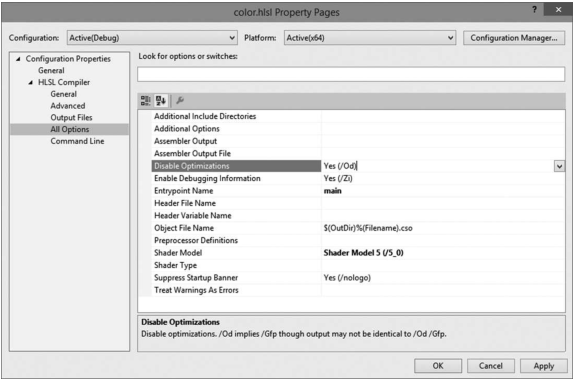
\includegraphics[width=\textwidth]{6-6}
    \centering
    \caption{添加一个自定义编译工具到项目中}
    \label{fig:6-6}
\end{figure}

使用VS集成HLSL支持的一个缺点是它只支持每个文件一个着色器程序。 因此,您不能将顶点和像素着色器存储在一个文件中。 此外,有时候我们希望使用不同的预处理器指令编译相同的着色器程序,以获得着色器的不同变体。 同样,这将不可能使用集成VS支持,因为它是每个.hlsl输入一个.cso输出。
\end{flushleft}

\section{光栅化器状态(Rasterizer State)}
\begin{flushleft}
虽然渲染管线的许多部分都是可编程的,但某些部分只能配置。 由D3D12\_RASTERIZER\_DESC结构表示的光栅化器状态组用于配置渲染管线的光栅化阶段:\\
\begin{lstlisting}
typedef struct D3D12_RASTERIZER_DESC
{
    D3D12_FILL_MODE FillMode;   // Default: D3D12_FILL_SOLID
    D3D12_CULL_MODE CullMode;   // Default: D3D12_CULL_BACK
    BOOL FrontCounterClockwise; // Default: false
    INT DepthBias;              // Default: 0
    FLOAT DepthBiasClamp;       // Default: 0.0f
    FLOAT SlopeScaledDepthBias; // Default: 0.0f
    BOOL DepthClipEnable;       // Default: true
    BOOL ScissorEnable;         // Default: false
    BOOL MultisampleEnable;     // Default: false
    BOOL AntialiasedLineEnable; // Default: false
    UINT ForcedSampleCount;     // Default: 0

    // Default: D3D12_CONSERVATIVE_RASTERIZATION_MODE_OFF
    D3D12_CONSERVATIVE_RASTERIZATION_MODE ConservativeRaster;
} D3D12_RASTERIZER_DESC;
\end{lstlisting}
这些成员大多数是高级选项或不经常使用;详细描述请参阅SDK文档。我们在这里只描述四个。\\
~\\
1.FillMode: 指定 D3D12\_FILL\_WIREFRAME 进行线框渲染或 D3D12\_FILL\_SOLID 用于实体渲染。固体渲染是默认的。\\
2.CullMode: 指定 D3D12\_CULL\_NONE 禁用剔除,D3D12\_CULL\_BACK 剔除背向三角形,或 D3D12\_CULL\_FRONT 剔除前向三角形。 背面三角形默认为剔除。\\
3.FrontCounterClockwise: 如果希望顺时针(相对于相机)顺时针排列的三角形被视为正面,并且逆时针(相对于相机)排列的三角形被视为背面,则指定false。 如果您希望将逆时针(相对于相机)排列的三角形视为正面,并将顺时针(相对于相机)排列的三角形视为背面,请指定true。 此状态默认为false。\\
4.ScissorEnable: 指定true以启用裁剪测试(第4.3.10节),如果为false则禁用它。 默认值是false。\\
~\\
以下代码表示如何创建打开线框模式并禁用背面剔除的栅格化状态:\\
\begin{lstlisting}
CD3DX12_RASTERIZER_DESC rsDesc(D3D12_DEFAULT);
rsDesc.FillMode = D3D12_FILL_WIREFRAME;
rsDesc.CullMode = D3D12_CULL_MODE;
\end{lstlisting}
CD3DX12\_RASTERIZER\_DESC 是一个便捷类,它扩展了 D3D12\_RASTERIZER\_DESC 并添加了一些辅助构造函数。 特别是,它有一个构造函数,它接受一个类型为 CD3D12\_DEFAULT 的对象,该对象只是一个用于重载的虚拟类型,用于将光栅化器状态成员初始化为默认值。CD3D12\_DEFAULT 和 D3D12\_DEFAULT 定义如下:\\
\begin{lstlisting}
struct CD3D12_DEFAULT {};
extern const DECLSPEC_SELECTANY CD3D12_DEFAULT D3D12_DEFAULT;
\end{lstlisting}
几个 Direct3D 便利类会使用 D3D12\_DEFAULT。
\end{flushleft}

\section{管道状态对象(Pipeline State Object)}
\begin{flushleft}
我们已经展示了如何描述输入布局描述,如何创建顶点和像素着色器,以及如何配置光栅器状态组。 但是,我们尚未显示如何将这些对象绑定到图形管道以供实际使用。 控制图形管道状态的大多数对象都被指定为一个称为管道状态对象(PSO)的聚合,它由 ID3D12PipelineState 接口表示。 为了创建一个PSO,我们首先通过填写一个D3D12\_GRAPHICS\_PIPELINE\_STATE\_DESC实例来描述它:\\
\end{flushleft}
\begin{lstlisting}
typedef struct D3D12_GRAPHICS_PIPELINE_STATE_DESC
{
    ID3D12RootSignature *pRootSignature;
    D3D12_SHADER_BYTECODE VS;
    D3D12_SHADER_BYTECODE PS;
    D3D12_SHADER_BYTECODE DS;
    D3D12_SHADER_BYTECODE HS;
    D3D12_SHADER_BYTECODE GS;
    D3D12_STREAM_OUTPUT_DESC StreamOutput;
    D3D12_BLEND_DESC BlendState;
    UINT SampleMask;
    D3D12_RASTERIZER_DESC RasterizerState;
    D3D12_DEPTH_STENCIL_DESC DepthStencilState;
    D3D12_INPUT_LAYOUT_DESC InputLayout;
    D3D12_PRIMITIVE_TOPOLOGY_TYPE PrimitiveTopologyType;
    UINT NumRenderTargets;
    DXGI_FORMAT RTVFormats[8];
    DXGI_FORMAT DSVFormat;
    DXGI_SAMPLE_DESC SampleDesc;
} D3D12_GRAPHICS_PIPELINE_STATE_DESC;
\end{lstlisting}
\begin{flushleft}
1.pRootSignature: 指向与此PSO绑定的根签名的指针。根签名必须与此PSO指定的着色器兼容。\\
2.VS: 要绑定的顶点着色器。 这由 D3D12\_SHADER\_BYTECODE 结构指定,该结构是指向编译的字节码数据的指针,以及字节码数据的大小(以字节为单位)。\\
3.PS: 要绑定的像素着色器。\\
4.DS: 要绑定的域着色器。(我们将在之后的章节讨论)\\
5.HS: 要绑定的外壳着色器。(我们将在之后的章节讨论)\\
6.GS: 要绑定的几何着色器。(我们将在之后的章节讨论)\\
7.StreamOutput: 用于称(流出)stream-out的高级技术。现在我们只是把这个领域归零(zero-out)。\\
8.BlendState: 指定配置混合的混合状态。 我们将在后面的章节中讨论这个状态组; 现在,指定默认 CD3DX12\_BLEND\_DESC(D3D12\_DEFAULT)。\\
9.SampleMask: 多重采样可能需要多达32个样本。 该32位整数值用于启用/禁用采样。 例如,如果关闭第5位,则第5个采样不会被采用。 当然,如果您实际使用至少5个采样的多重采样,则禁用第5个采样只会产生任何结果。 如果应用程序使用单个采样,则只有该参数的第一位很重要。 通常使用默认的0xffffffff,这不会禁用任何样本。\\
10.RasterizerState: 指定配置光栅化器的光栅化状态。\\
11.DepthStencilState: 指定配置深度/模板测试的深度/模板状态。 我们将在后面的章节中讨论这个状态组; 现在,指定默认CD3DX12\_DEPTH\_STENCIL\_DESC(D3D12\_DEFAULT)。
12.InputLayout: 输入布局描述,它只是D3D12\_INPUT\_ELEMENT\_DESC元素的一个数组,以及数组中的元素数。\\
\begin{lstlisting}
typedef struct D3D12_INPUT_LAYOUT_DESC
{
    const D3D12_INPUT_ELEMENT_DESC *pInputElementDescs;
    UINT NumElements;
} D3D12_INPUT_LAYOUT_DESC;
\end{lstlisting}
13.PrimitiveTopologyType: 指定原始拓扑类型。\\
\begin{lstlisting}
typedef enum D3D12_PRIMITIVE_TOPOLOGY_TYPE
{
    D3D12_PRIMITIVE_TOPOLOGY_TYPE_UNDEFINED = 0,
    D3D12_PRIMITIVE_TOPOLOGY_TYPE_POINT = 1,
    D3D12_PRIMITIVE_TOPOLOGY_TYPE_LINE = 2,
    D3D12_PRIMITIVE_TOPOLOGY_TYPE_TRIANGLE = 3,
    D3D12_PRIMITIVE_TOPOLOGY_TYPE_PATCH = 4
} D3D12_PRIMITIVE_TOPOLOGY_TYPE;
\end{lstlisting}
14.NumRenderTargets: 我们正在同时使用的渲染目标的数量。\\
15.RTVFormats: 呈现目标格式。 这是一个支持同时写入多个渲染目标的数组。 这应该与我们使用PSO的渲染目标的设置相匹配。\\
16.DSVFormat: 深度/模板缓冲区的格式。 这应该与我们使用PSO的深度/模板缓冲区的设置匹配。\\
17.SampleDesc: 介绍多重采样计数和质量级别。 这应该与我们正在使用的渲染目标的设置相匹配。\\
~\\
在我们填写完一个 D3D12\_GRAPHICS\_PIPELINE\_STATE\_DESC 实例后,我们使用 ID3D12Device::CreateGraphicsPipelineState 方法创建一个 ID3D12PipelineState 对象:\\
\begin{lstlisting}
ComPtr<ID3D12RootSignature> mRootSignature;
std::vector<D3D12_INPUT_ELEMENT_DESC> mInputLayout;
ComPtr<ID3DBlob> mvsByteCode;
ComPtr<ID3DBlob> mpsByteCode;
...
D3D12_GRAPHICS_PIPELINE_STATE_DESC psoDesc;
ZeroMemory(&psoDesc, 
           sizeof(D3D12_GRAPHICS_PIPELINE_STATE_DESC));
psoDesc.InputLayout = {
    mInputLayout.data(),
   (UINT)mInputLayout.size()
};
psoDesc.pRootSignature = mRootSignature.Get();
psoDesc.VS = {
    reinterpret_cast<BYTE*>(mvsByteCode->GetBufferPointer()),
    mvsByteCode->GetBufferSize()
};
psoDesc.PS = {
    reinterpret_cast<BYTE*>(mpsByteCode->GetBufferPointer()),
    mpsByteCode->GetBufferSize()
};
psoDesc.RasterizerState = CD3D12_RASTERIZER_DESC(D3D12_DEFAULT);
psoDesc.BlendState = CD3D12_BLEND_DESC(D3D12_DEFAULT);
psoDesc.DepthStencilState = CD3D12_DEPTH_STENCIL_DESC(D3D12_DEFAULT);
psoDesc.SampleMask = UINT_MAX;
psoDesc.PrimitiveTopologyType = D3D12_PRIMITIVE_TOPOLOGY_TYPE_TRIANGLE;
psoDesc.NumRenderTargets = 1;
psoDesc.RTVFormats[0] = mBackBufferFormat;
psoDesc.SampleDesc.Count = m4xMsaaState ? 4 : 1;
psoDesc.SampleDesc.Quality = m4xMsaaState ? (m4xMsaaQuality - 1) : 0;
psoDesc.DSVFormat = mDepthStencilFormat;

ComPtr<ID3D12PipelineState> mPSO;
md3dDevice->CreateGraphicsPipelineState(&psoDesc,IID_PPV_ARGS(&mPSO)));
\end{lstlisting}
上述代码用 ID3D12PipelineState 对象聚合(aggregate)了很多状态,出于性能考虑,我们指定所有这些对象都作为一个聚合传递到图形管线中。通过将它们作为聚合,Direct3D可以验证所有状态是否兼容,驱动程序可以预先生成所有代码以编写硬件状态。在Direct3D 11状态模型中,这些渲染状态片段是分开设置的。但是,各个状态是相关的; 如果一个状态被改变,它可能会另外要求驱动程序重新编程硬件以获取另一个依赖状态。由于配置流水线的许多状态会被改变,所以硬件的状态可能会被多次重新编写。为了避免这种情况,驱动程序通常推迟对硬件状态进行编写,直到在整个管道状态将被知道时发出绘制调用。但是这种延期需要驱动在运行时进行额外的记录工作; 它需要跟踪哪些状态发生了变化,然后生成代码以在运行时对硬件状态进行编程。 在新的Direct3D 12模型中,驱动程序可以在初始化时生成编程流水线状态所需的所有代码,因为我们将大部分流水线状态指定为聚合。\\
~\\
NOTICE:由于PSO验证和创建可能非常耗时,PSO应该在初始化时生成。 对此的一个例外可能是在运行时第一次引用PSO时创建PSO; 然后将其存储在哈希表等集合中,以便将来可以快速获取以供将来使用。\\
~\\
并非所有渲染状态都封装在PSO中。 一些像视口和裁剪矩形的状态是独立于PSO的。 这种状态可以独立于另一个管道状态而有效地设置,因此将它们包含在PSO中没有任何优势。\\
Direct3D基本上是一个状态机。 在我们改变它们之前,事物会保持现状。 如果您正在绘制的某些对象使用一个PSO,并且您正在绘制的其他对象需要不同的PSO,那么您需要像这样构造代码:\\
\begin{lstlisting}
// Reset specifies initial PSO.
mCommandList->Reset(mDirectCmdListAlloc.Get(), mPSO1.Get());
/*...draw objects using PSO 1...*/
// Change PSO
mCommandList->SetPipelineState(mPSO2.Get());
/*...draw objects using PSO 2...*/
// Change PSO
mCommandList->SetPipelineState(mPSO3.Get());
/*...draw objects using PSO 3...*/
\end{lstlisting}
换句话说,当PSO绑定到命令列表时,它不会改变,直到你覆盖它(或命令列表被重置)。\\
~\\
NOTICE: 出于性能考虑,PSO状态变化应该保持在最小。 一起绘制可以使用相同PSO的所有对象。 不要更改每次绘制调用的PSO!
\end{flushleft}

\section{几何工具结构体(Geometry Helper Structure)}
\begin{flushleft}
创建一个将顶点和索引缓冲区组合在一起以定义一组几何体的结构会很有帮助。 另外,这种结构可以保留顶点和索引数据的系统内存支持,以便可以由CPU读取。 CPU将需要访问几何数据以进行拾取和碰撞检测等操作。 另外,结构缓存顶点和索引缓冲区的重要属性,如格式和碰撞,并提供返回视图到缓冲区的方法。 每当我们定义一个几何体块时,我们在整本书中使用下面的MeshGeometry(在d3dUtil.h中定义)结构。\\
\begin{lstlisting}
// Defines a subrange of geometry in a MeshGeometry. This is for when
// multiple geometries are stored in one vertex and index buffer. It
// provides the offsets and data needed to draw a subset of geometry
// stores in the vertex and index buffers so that we can implement the
// technique described by Figure \ref{fig:6-3}.
struct SubmeshGeometry
{
    UINT IndexCount = 0;
    UINT StartIndexLocation = 0;
    INT  BaseVertexLocation = 0;

    // Bounding box of the geometry defined by this submesh.
    // This is used in later chapters of the book.
    DirectX::BoundingBox Bounds;
};

struct MeshGeometry
{
    // Give it a name so we can look it up by name.
    std::string Name;

    // System memory copies. Use Blobs because the vertex/index format can
    // be generic.
    // It is up to the client to cast appropriately.
    Microsoft::WRL::ComPtr<ID3DBlob> VertexBufferCPU = nullptr;
    Microsoft::WRL::ComPtr<ID3DBlob> IndexBufferCPU = nullptr;

    Microsoft::WRL::ComPtr<ID3D12Resource> VertexBufferGPU = nullptr;
    Microsoft::WRL::ComPtr<ID3D12Resource> IndexBufferGPU = nullptr;
    
    Microsoft::WRL::ComPtr<ID3D12Resource> VertexBufferUploader = nullptr;
    Microsoft::WRL::ComPtr<ID3D12Resource> IndexBufferUploader = nullptr;
    
    // Data about the buffers
    UINT VertexByteStride = 0;
    UINT VertexBufferByteSize = 0;
    DXGI_FORMAT IndexFormat = DXGI_FORMAT_R16_UINT;
    UINT IndexBufferByteSize = 0;
    
    // A MeshGeometry may store multiple geometries in one vertex/index
    // buffer.
    // Use this container to define the Submesh geometries so we can draw
    // the Submeshes individually.
    std::unordered_map<std::string, SubmeshGeometry> DrawArgs;
    
    D3D12_VERTEX_BUFFER_VIEW VertexBufferView() const
    {
        D3D12_VERTEX_BUFFER_VIEW vbv;
        vbv.BufferLocation = VertexBufferGPU->GetGPUVirtualAddress();
        vbv.StrideInBytes = VertexByteStride;
        vbv.SizeInBytes = VertexBufferByteSize;

        return vbv;
    }
    
    D3D12_INDEX_BUFFER_VIEW IndexBufferView() const
    {
        D3D12_INDEX_BUFFER_VIEW ibv;
        ibv.BufferLocation = IndexBufferGPU->GetGPUVirtualAddress();
        ibv.Format = IndexFormat;
        ibv.SizeInBytes = IndexBufferByteSize;

        return ibv;
    }
    
    // We can free this memory after we finish upload to the GPU.
    void DisposeUploaders()
    {
       VertexBufferUploader = nullptr;
       IndexBufferUploader = nullptr;
    }
};
\end{lstlisting}
\end{flushleft}

\section{BOX DEMO}

\chapter{在Direct3D中绘制2(Drawing in Direct3D Part 2)}
\begin{flushleft}
本章介绍我们将在本书其余部分使用的一些绘图模式。 本章首先介绍一种绘图优化的方法,我们将其称为“帧资源”。使用帧资源,我们修改渲染循环,这样我们就不必每帧刷新命令队列; 这提高了CPU和GPU的利用率。 接下来,我们介绍渲染项的概念,并解释我们如何根据更新频率划分常量数据。 此外,我们更详细地检查根签名,并了解其他根参数类型:根描述符和根常量。 最后,我们展示了如何绘制一些更复杂的对象; 到本章结束时,您将能够绘制类似丘陵和山谷,圆柱体,球体和动画波浪模拟的表面。\\
~\\
{\large Objectives:}
\begin{itemize}
    \item 了解对渲染过程的修改,不要求我们每帧刷新命令队列,从而提高性能。
    \item 了解其他两种类型的根签名参数类型:根描述符和根常量。
    \item 探索如何在程序上生成和绘制常见的几何形状,如网格,圆柱体和球体。
    \item 了解我们如何在CPU上设置顶点动画并使用动态顶点缓冲区将新顶点位置上传到GPU。
\end{itemize}
\end{flushleft}

%---- 7.1 ------
\section{帧资源(Frame Resources)}
\begin{flushleft}
回忆 4.2 节,CPU和GPU并行工作。 CPU构建并提交命令列表(除了其他CPU工作之外),GPU处理命令队列中的命令。 目标是让CPU和GPU忙碌,以充分利用系统上可用的硬件资源。 到目前为止,在我们的演示中,我们已经每帧同步CPU和GPU一次。 两个例子解释这种同步的必要性:\\
\begin{itemize}
    \item 1.在GPU完成执行命令之前,不能重置命令分配器(command allocator)。 假设我们没有进行同步,以便CPU在GPU处理完当前帧n之前可以继续下一帧n + 1:如果CPU在帧n + 1中重置命令分配器,但GPU仍在处理命令 从第n帧开始,我们将清除GPU仍在使用的命令。
    \item 2.在GPU完成执行引用常量缓冲区的绘图命令之前,CPU无法更新常量缓冲区。 此示例对应于4.2.2节和图4.7中描述的情况。 假设我们没有进行同步,以便CPU在GPU完成处理当前帧n之前可以继续下一帧n + 1:如果CPU在帧n + 1中覆盖常量缓冲区数据,但GPU还没有 执行引用帧n中的常量缓冲区的绘制调用,然后常量缓冲区包含当GPU执行帧n的绘制调用时的错误数据。
\end{itemize}
因此,我们一直在每帧结束时调用 D3DApp::FlushCommandQueue,以确保GPU已完成执行帧的所有命令。 此解决方案有效,但由于以下原因效率低下:\\
\begin{itemize}
    \item 1.在帧开始时,GPU将不会有任何要处理的命令,因为我们等待清空命令队列。 它必须等到CPU构建并提交一些命令才能执行。
    \item 2.在帧结束时,CPU正在等待GPU完成处理命令。
\end{itemize}
所以每一帧,CPU和GPU都会在某些时候空闲。\\
~\\
该问题的一个解决方案是创建CPU修改每个帧所需的资源的循环数组。 我们称这种资源为帧资源,我们通常使用三个帧资源元素的循环数组。 对于帧n,CPU将循环通过帧资源队列以获得下一个可用(即,未被GPU使用)帧资源。 然后,CPU将执行任何资源更新,并在GPU处理先前帧时构建和提交帧n的命令列表。 然后CPU继续进行第n + 1帧并重复。 如果帧资源阵列有三个元素,这可以使CPU在GPU之前达到两帧,从而确保GPU保持忙碌状态。 下面是我们在本章中用于“Shapes”演示的帧资源类的示例。 由于CPU只需要在此演示中修改常量缓冲区,因此帧资源类仅包含常量缓冲区。\\
\end{flushleft}
\begin{lstlisting}
// Stores the resources needed for the CPU to build
// the command lists
// for a frame. The contents here will vary from app
// to app based on
// the needed resources.
struct FrameResource
{
public:
    FrameResource(ID3D12Device* device, UINT passCount, UINT objectCount);
    FrameResource(const FrameResource& rhs) = delete;
    FrameResource& operator=(const FrameResource& rhs) = delete;
    ~FrameResource();
    // We cannot reset the allocator until the GPU is
    // done processing the
    // commands. So each frame needs their own
    // allocator.
    Microsoft::WRL::ComPtr<ID3D12CommandAllocator> CmdListAlloc;
    
    // We cannot update a cbuffer until the GPU is done
    // processing the
    // commands that reference it. So each frame needs
    // their own cbuffers.
    std::unique_ptr<UploadBuffer<PassConstants>> PassCB = nullptr;
    std::unique_ptr<UploadBuffer<ObjectConstants>>
    ObjectCB = nullptr;
    // Fence value to mark commands up to this fence
    // point. This lets us
    // check if these frame resources are still in use
    // by the GPU.
    UINT64 Fence = 0;
};

FrameResource::FrameResource(ID3D12Device* device,
                             UINT passCount, UINT
                             objectCount)
{
    ThrowIfFailed(device->CreateCommandAllocator(
        D3D12_COMMAND_LIST_TYPE_DIRECT,
        IID_PPV_ARGS(CmdListAlloc.GetAddressOf())));
    PassCB = std::make_unique<UploadBuffer<PassConstants>>(
        device,
        passCount, 
        true);
    ObjectCB = std::make_unique<UploadBuffer<ObjectConstants>>(
        device,
        objectCount, true);
}
FrameResource::˜FrameResource() {}
\end{lstlisting}
\begin{flushleft}
然后,我们的应用程序类将三个帧资源的向量实例化,并设置成员变量以跟踪当前帧资源:\\
\end{flushleft}
\begin{lstlisting}
static const int NumFrameResources = 3;
std::vector<std::unique_ptr<FrameResource>> mFrameResources;
FrameResource* mCurrFrameResource = nullptr;
int mCurrFrameResourceIndex = 0;
void ShapesApp::BuildFrameResources()
{
    for(int i = 0; i < gNumFrameResources; ++i)
    {
        mFrameResources.push_back(std::make_unique<FrameResource>(
                                      md3dDevice.Get(), 
                                      1, 
                                      (UINT)mAllRitems.size()));
    }
}
\end{lstlisting}
\begin{flushleft}
现在,对于CPU帧n,算法的工作原理如下:\\
\end{flushleft}
\begin{lstlisting}
void ShapesApp::Update(const GameTimer& gt)
{
    // Cycle through the circular frame resource array.
    mCurrFrameResourceIndex = (mCurrFrameResourceIndex + 1) % NumFrameResources;
    mCurrFrameResource = mFrameResources[mCurrFrameResourceIndex];
    // Has the GPU finished processing the commands of
    // the current frame
    // resource. If not, wait until the GPU has
    // completed commands up to
    // this fence point.
    if(mCurrFrameResource->Fence != 0 &&
       mCommandQueue->GetLastCompletedFence() < mCurrFrameResource->Fence)
    {
        HANDLE eventHandle = CreateEventEx(nullptr, false, 
                                  false, EVENT_ALL_ACCESS);
        ThrowIfFailed(mCommandQueue->SetEventOnFenceCompletion(
             mCurrFrameResource->Fence, eventHandle));
        WaitForSingleObject(eventHandle, INFINITE);
        CloseHandle(eventHandle);
    }
    // […] Update resources in mCurrFrameResource (like cbuffers).
}
void ShapesApp::Draw(const GameTimer& gt)
{
    // […] Build and submit command lists for this frame.
    // Advance the fence value to mark commands up to
    // this fence point.
    mCurrFrameResource->Fence = ++mCurrentFence;
    // Add an instruction to the command queue to set a
    // new fence point.
    // Because we are on the GPU timeline, the new fence
    // point won’t be
    // set until the GPU finishes processing all the
    // commands prior to
    // this Signal().
    mCommandQueue->Signal(mFence.Get(), mCurrentFence);
    // Note that GPU could still be working on commands
    // from previous
    // frames, but that is okay, because we are not
    // touching any frame
    // resources associated with those frames.
}
\end{lstlisting}
\begin{flushleft}
请注意,此解决方案不会阻止等待。 如果一个处理器处理帧的速度比另一个处理器快得多,那么一个处理器最终将不得不等待另一个处理器赶上,因为我们不能让一个处理器远远超过另一个处理器。 如果GPU处理命令的速度比CPU提交工作的速度快,那么GPU将处于空闲状态。 一般来说,如果我们试图推动图形限制,我们希望避免这种情况,因为我们没有充分利用GPU。 另一方面,如果CPU总是以比GPU更快的速度处理帧,那么CPU将不得不在某个时刻等待。 这是理想的情况,因为GPU正在被充分利用; 额外的CPU周期总是可以用于游戏的其他部分,如AI,物理和游戏逻辑。\\
因此,如果多个帧资源不能阻止任何等待,它对我们有何帮助? 它可以帮助我们保持GPU的供给。 当GPU正在处理来自帧n的命令时,它允许CPU继续构建和提交帧n + 1和n + 2的命令。 这有助于保持命令队列非空,以便GPU始终有工作要做。
\end{flushleft}

%---- 7.2 ------
\section{渲染项(Render Items)}
\begin{flushleft}
绘制对象需要设置多个参数,例如绑定顶点和索引缓冲区,绑定对象常量,设置基本类型(primitive type)以及指定DrawIndexedInstanced参数。 当我们开始在场景中绘制更多对象时,创建一个存储绘制对象所需数据的轻量级结构会很有帮助。 这些数据因应用程序而异,因为我们添加了需要不同绘图数据的新功能。 我们将提交完整绘制所需的数据集称为渲染管道渲染项。 对于此演示,我们的RenderItem结构如下所示:\\
\end{flushleft}
\begin{lstlisting}
// Lightweight structure stores parameters to draw a shape.  This will
// vary from app-to-app.
struct RenderItem
{
    RenderItem() = default;

    // World matrix of the shape that describes the object's local space
    // relative to the world space, which defines the position, orientation,
    // and scale of the object in the world.
    XMFLOAT4X4 World = MathHelper::Identity4x4();

    // Dirty flag indicating the object data has changed 
    // and we need to update the constant buffer.
    // Because we have an object cbuffer for each FrameResource, 
    // we have to apply the update to each FrameResource.  
    // Thus, when we modify obect data we should set 
    // NumFramesDirty = gNumFrameResources so that each 
    // frame resource gets the update.
    int NumFramesDirty = gNumFrameResources;

    // Index into GPU constant buffer corresponding to 
    // the ObjectCB for this render item.
    UINT ObjCBIndex = -1;

    MeshGeometry* Geo = nullptr;

    // Primitive topology.
    D3D12_PRIMITIVE_TOPOLOGY PrimitiveType = D3D_PRIMITIVE_TOPOLOGY_TRIANGLELIST;

    // DrawIndexedInstanced parameters.
    UINT IndexCount = 0;
    UINT StartIndexLocation = 0;
    int BaseVertexLocation = 0;
};
\end{lstlisting}
\begin{flushleft}
我们的应用程序将根据需要绘制的方式维护渲染项目列表; 也就是说,需要不同PSO的渲染项目将保存在不同的列表中。\\
\end{flushleft}
\begin{lstlisting}
// List of all the render items.
std::vector<std::unique_ptr<RenderItem>> mAllRitems;
// Render items divided by PSO.
std::vector<RenderItem*> mOpaqueRitems;
std::vector<RenderItem*> mTransparentRitems;
\end{lstlisting}

%---- 7.3 ------
\section{传递常量(Pass Constants)}
\begin{flushleft}
NOTICE: Pass Constants 这是一整个名词。该常量用于存储额外信息\\
~\\
从上一节中可以看出,我们在FrameResource类中引入了一个新的常量缓冲区:
\end{flushleft}
\begin{lstlisting}
std::unique_ptr<UploadBuffer<PassConstants>> PassCB = nullptr;
\end{lstlisting}
\begin{flushleft}
在演示中,此缓冲区存储在给定渲染过程中固定的常量数据,例如眼睛位置,视图和投影矩阵,以及有关屏幕(渲染目标)尺寸的信息; 它还包括游戏计时信息,这是在着色器程序中可以访问的有用数据。 请注意,我们的演示不一定会使用所有这些常量数据,我们可以方便地使用这些数据,并且提供额外数据的成本很低。 例如,虽然我们现在不需要渲染目标大小,但是当我们实现一些后期处理效果时,将需要具有该信息。
\end{flushleft}
\begin{lstlisting}
cbuffer cbPass : register(b1)
{
    float4x4 gView;
    float4x4 gInvView;
    float4x4 gProj;
    float4x4 gInvProj;
    float4x4 gViewProj;
    float4x4 gInvViewProj;
    float3   gEyePosW;
    float    cbPerObjectPad1;
    float2   gRenderTargetSize;
    float2   gInvRenderTargetSize;
    float    gNearZ;
    float    gFarZ;
    float    gTotalTime;
    float    gDeltaTime;
};
\end{lstlisting}
\begin{flushleft}
我们还修改了每个对象常量缓冲区,仅存储与对象关联的常量。 到目前为止,我们与绘图对象关联的唯一常量数据是其世界矩阵:
\end{flushleft}
\begin{lstlisting}
cbuffer cbPerObject : register(b0)
{
    float4x4 gWorld;
};
\end{lstlisting}
\begin{flushleft}
这些更改是根据更新频率对常量进行分组。 每次通过常量只需要在每次渲染过程中更新一次,并且对象常量只需要在对象的世界矩阵发生变化时进行更改。如果我们在场景中有一个静态对象,就像一棵树,我们只需要将其世界矩阵设置一次到一个常量缓冲区,然后再也不要更新常量缓冲区。 在我们的演示中,我们实现了以下方法来处理每次传递和每个对象常量缓冲区的更新。Update方法中每帧调用一次这些方法。
\end{flushleft}
\begin{lstlisting}
void ShapesApp::UpdateObjectCBs(const GameTimer& gt)
{
    auto currObjectCB = mCurrFrameResource->ObjectCB.get();
    for(auto& e : mAllRitems)
    {
        // Only update the cbuffer data if the constants have changed.  
        // This needs to be tracked per frame resource.
        if(e->NumFramesDirty > 0)
        {
            XMMATRIX world = XMLoadFloat4x4(&e->World);

            ObjectConstants objConstants;
            XMStoreFloat4x4(&objConstants.World, XMMatrixTranspose(world));

            currObjectCB->CopyData(e->ObjCBIndex, objConstants);

            // Next FrameResource need to be updated too.
            e->NumFramesDirty--;
        }
    }
}

void ShapesApp::UpdateMainPassCB(const GameTimer& gt)
{
    XMMATRIX view = XMLoadFloat4x4(&mView);
    XMMATRIX proj = XMLoadFloat4x4(&mProj);

    XMMATRIX viewProj = XMMatrixMultiply(view, proj);
    XMMATRIX invView = XMMatrixInverse(&XMMatrixDeterminant(view), view);
    XMMATRIX invProj = XMMatrixInverse(&XMMatrixDeterminant(proj), proj);
    XMMATRIX invViewProj = XMMatrixInverse(&XMMatrixDeterminant(viewProj), viewProj);

    XMStoreFloat4x4(&mMainPassCB.View, XMMatrixTranspose(view));
    XMStoreFloat4x4(&mMainPassCB.InvView, XMMatrixTranspose(invView));
    XMStoreFloat4x4(&mMainPassCB.Proj, XMMatrixTranspose(proj));
    XMStoreFloat4x4(&mMainPassCB.InvProj, XMMatrixTranspose(invProj));
    XMStoreFloat4x4(&mMainPassCB.ViewProj, XMMatrixTranspose(viewProj));
    XMStoreFloat4x4(&mMainPassCB.InvViewProj, XMMatrixTranspose(invViewProj));
    mMainPassCB.EyePosW = mEyePos;
    mMainPassCB.RenderTargetSize = XMFLOAT2((float)mClientWidth, (float)mClientHeight);
    mMainPassCB.InvRenderTargetSize = XMFLOAT2(1.0f / mClientWidth, 1.0f / mClientHeight);
    mMainPassCB.NearZ = 1.0f;
    mMainPassCB.FarZ = 1000.0f;
    mMainPassCB.TotalTime = gt.TotalTime();
    mMainPassCB.DeltaTime = gt.DeltaTime();

    auto currPassCB = mCurrFrameResource->PassCB.get();
    currPassCB->CopyData(0, mMainPassCB);
}
\end{lstlisting}
\begin{flushleft}
我们相应地更新顶点着色器以支持这些常量缓冲区更改:\\
\end{flushleft}
\begin{lstlisting}
VertexOut VS(VertexIn vin)
{
    VertexOut vout;
    // Transform to homogeneous clip space.
    float4 posW = mul(float4(vin.PosL, 1.0f), gWorld);
    vout.PosH = mul(posW, gViewProj);
    // Just pass vertex color into the pixel shader.
    vout.Color = vin.Color;
    return vout;
}
\end{lstlisting}
\begin{flushleft}
这种调整每个顶点的额外矢量矩阵乘法在具有充足计算能力的现代GPU上可以忽略不计。\\
~\\
我们的着色器所期望的资源已经改变了; 因此,我们需要相应地更新根签名以获取两个描述符表(我们需要两个表,因为CBV将被设置为不同的频率 - 每次传递CBV仅需要在每个渲染过程中设置一次,而每个对象CBV需要 每个渲染项设置):
\end{flushleft}
\begin{lstlisting}
void ShapesApp::BuildRootSignature()
{
    CD3DX12_DESCRIPTOR_RANGE cbvTable0;
    cbvTable0.Init(D3D12_DESCRIPTOR_RANGE_TYPE_CBV, 1, 0);

    CD3DX12_DESCRIPTOR_RANGE cbvTable1;
    cbvTable1.Init(D3D12_DESCRIPTOR_RANGE_TYPE_CBV, 1, 1);

    // Root parameter can be a table, root descriptor or root constants.
    CD3DX12_ROOT_PARAMETER slotRootParameter[2];

    // Create root CBVs.
    slotRootParameter[0].InitAsDescriptorTable(1, &cbvTable0);
    slotRootParameter[1].InitAsDescriptorTable(1, &cbvTable1);

    // A root signature is an array of root parameters.
    CD3DX12_ROOT_SIGNATURE_DESC rootSigDesc(2, slotRootParameter, 0, nullptr, 
        D3D12_ROOT_SIGNATURE_FLAG_ALLOW_INPUT_ASSEMBLER_INPUT_LAYOUT);

    // create a root signature with a single slot which points to a descriptor range consisting of a single constant buffer
    ComPtr<ID3DBlob> serializedRootSig = nullptr;
    ComPtr<ID3DBlob> errorBlob = nullptr;
    HRESULT hr = D3D12SerializeRootSignature(&rootSigDesc, D3D_ROOT_SIGNATURE_VERSION_1,
        serializedRootSig.GetAddressOf(), errorBlob.GetAddressOf());

    if(errorBlob != nullptr)
    {
        ::OutputDebugStringA((char*)errorBlob->GetBufferPointer());
    }
    ThrowIfFailed(hr);

    ThrowIfFailed(md3dDevice->CreateRootSignature(
        0,
        serializedRootSig->GetBufferPointer(),
        serializedRootSig->GetBufferSize(),
        IID_PPV_ARGS(mRootSignature.GetAddressOf())));
}
\end{lstlisting}
\begin{flushleft}
NOTICE: 不要过多地使用着色器中的常量缓冲区数量。 [Thibieroz13]建议您将它们保持在5以下以保持性能。
\end{flushleft}

%---- 7.4 ------
\section{图形集合(Shape Geometry)}
\begin{flushleft}
在本节中,我们将展示如何为椭圆体,球体,圆柱体和圆锥体创建几何体。 这些形状对于绘制天空圆顶,调试,可视化碰撞检测和延迟渲染非常有用。 例如,您可能希望将所有游戏角色渲染为调试测试的球体。\\
~\\
我们将过程几何生成代码放在GeometryGenerator类(GeometryGenerator.h / .cpp)中。 GeometryGenerator是一个实用程序类,用于生成简单的几何形状,如网格,球体,圆柱体和盒子,我们在本书中将它们用于演示程序。 这个类在系统内存中生成数据,然后我们必须将我们想要的数据复制到顶点和索引缓冲区。 GeometryGenerator会创建一些将在后面的章节中使用的顶点数据。 我们当前的演示中不需要这些数据,因此我们不会将此数据复制到顶点缓冲区中。 MeshData结构是嵌套在GeometryGenerator中的简单结构,它存储顶点和索引列表:\\
\end{flushleft}
\begin{lstlisting}
class GeometryGenerator
{
public:
    using uint16 = std::uint16_t;
    using uint32 = std::uint32_t;

    struct Vertex
    {
        Vertex(){}
        Vertex(
            const DirectX::XMFLOAT3& p, 
            const DirectX::XMFLOAT3& n, 
            const DirectX::XMFLOAT3& t, 
            const DirectX::XMFLOAT2& uv) :
            Position(p), 
            Normal(n), 
            TangentU(t), 
            TexC(uv){}
        Vertex(
            float px, float py, float pz, 
            float nx, float ny, float nz,
            float tx, float ty, float tz,
            float u, float v) : 
            Position(px,py,pz), 
            Normal(nx,ny,nz),
            TangentU(tx, ty, tz), 
            TexC(u,v){}

        DirectX::XMFLOAT3 Position;
        DirectX::XMFLOAT3 Normal;
        DirectX::XMFLOAT3 TangentU;
        DirectX::XMFLOAT2 TexC;
    };

    struct MeshData
    {
        std::vector<Vertex> Vertices;
        std::vector<uint32> Indices32;

        std::vector<uint16>& GetIndices16()
        {
            if(mIndices16.empty())
            {
                mIndices16.resize(Indices32.size());
                for(size_t i = 0; i < Indices32.size(); ++i)
                    mIndices16[i] = static_cast<uint16>(Indices32[i]);
            }

            return mIndices16;
        }

    private:
        std::vector<uint16> mIndices16;
    };
......
};
\end{lstlisting}
%---- 7.4.1 ----
\subsection{创建圆柱体网格(Generating a Cylinder Mesh)}
\begin{flushleft}
我们通过指定圆柱体的底部和顶部半径,高度以及切片和堆叠数来定义圆柱体,如图\ref{fig:7-1}所示。 我们将圆柱体分成三个部分:1)侧面几何形状,2)顶盖几何形状,以及3)底盖几何形状。
\end{flushleft}
\begin{figure}[h]
    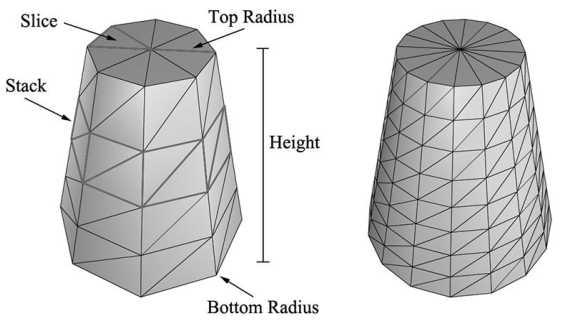
\includegraphics[width=\textwidth]{7-1}
    \centering
    \caption{在此图中,左侧的圆柱体有八个切片和四个堆叠,右侧的圆柱体有十六个切片和八个堆叠。 切片和堆栈控制三角形密度。 请注意,顶部和底部半径可以不同,以便我们可以创建锥形对象,而不仅仅是“纯”圆柱体。}
    \label{fig:7-1}
\end{figure}

%---- 7.4.1.1 ----
\subsubsection{圆柱体边缘几何(Cylinder Side Geometry)}
\begin{flushleft}
我们生成以原点为中心的圆柱体,平行于$y$轴。 从图\ref{fig:7-1}中,所有顶点都位于圆柱体的“环”上,其中有stackCount + 1个环,每个环都有 sliceCount 个(唯一)顶点。 连续环之间的半径差异为$\Delta r=(topRadius - bottomRadius)/ stackCount$。 如果我们从索引为0的底环开始,那么第i个环的半径是$r_{i} = bottomRadius + i\Delta r$,第i个环的高度是 $h_{i}=-\frac{h}{2}+i\Delta h$其中$\Delta h$是堆栈高度,h是圆柱高度。 因此,基本思想是迭代每个环,并生成位于该环上的顶点。 这给出了以下实现:\\
\end{flushleft}
\begin{lstlisting}
GeometryGenerator::MeshData 
GeometryGenerator::CreateCylinder(
    float bottomRadius, 
    float topRadius, 
    float height, 
    uint32 sliceCount, 
    uint32 stackCount)
{
    MeshData meshData;

    //
    // Build Stacks.
    // 

    float stackHeight = height / stackCount;

    // Amount to increment radius as we move up 
    // each stack level from bottom to top.
    float radiusStep = (topRadius - bottomRadius) / stackCount;

    uint32 ringCount = stackCount+1;

    // Compute vertices for each stack ring 
    // starting at the bottom and moving up.
    for(uint32 i = 0; i < ringCount; ++i)
    {
        float y = -0.5f*height + i*stackHeight;
        float r = bottomRadius + i*radiusStep;

        // vertices of ring
        float dTheta = 2.0f*XM_PI/sliceCount;
        for(uint32 j = 0; j <= sliceCount; ++j)
        {
            Vertex vertex;

            float c = cosf(j*dTheta);
            float s = sinf(j*dTheta);

            vertex.Position = XMFLOAT3(r*c, y, r*s);

            vertex.TexC.x = (float)j/sliceCount;
            vertex.TexC.y = 1.0f - (float)i/stackCount;

            // Cylinder can be parameterized as follows, where we introduce v
            // parameter that goes in the same direction as the v tex-coord
            // so that the bitangent goes in the same direction 
            // as the v tex-coord.
            //   Let r0 be the bottom radius and let r1 be the top radius.
            //   y(v) = h - hv for v in [0,1].
            //   r(v) = r1 + (r0-r1)v
            //
            //   x(t, v) = r(v)*cos(t)
            //   y(t, v) = h - hv
            //   z(t, v) = r(v)*sin(t)
            // 
            //  dx/dt = -r(v)*sin(t)
            //  dy/dt = 0
            //  dz/dt = +r(v)*cos(t)
            //
            //  dx/dv = (r0-r1)*cos(t)
            //  dy/dv = -h
            //  dz/dv = (r0-r1)*sin(t)

            // This is unit length.
            vertex.TangentU = XMFLOAT3(-s, 0.0f, c);

            float dr = bottomRadius-topRadius;
            XMFLOAT3 bitangent(dr*c, -height, dr*s);

            XMVECTOR T = XMLoadFloat3(&vertex.TangentU);
            XMVECTOR B = XMLoadFloat3(&bitangent);
            XMVECTOR N = XMVector3Normalize(XMVector3Cross(T, B));
            XMStoreFloat3(&vertex.Normal, N);

            meshData.Vertices.push_back(vertex);
        }
    }
......
\end{lstlisting}
\begin{flushleft}
NOTICE: 观察到每个环的第一个和最后一个顶点在位置上重复,但纹理坐标不重复。 我们必须这样做,以便我们可以正确地将纹理应用于圆柱体。\\
~\\
NOTICE: 实际上GeometryGenerator::CreateCylinder创建了额外的顶点数据,例如法线向量和纹理坐标,这些对未来的演示非常有用。 现在不要担心这些数量。\\
~\\
从图\ref{fig:7-2}可以看出,每个堆栈中的每个切片都有一个四边形(两个三角形)。 图\ref{fig:7-2}显示第$i$个堆栈和第$j$个切片的索引由下式给出:\\
\end{flushleft}
\begin{align*}
\Delta ABC = (i\cdot n+j, (i+1)\cdot n+j,(i+1)\cdot n+j+1)\\
\Delta ACD = (i\cdot n+j, (i+1)\cdot n+j+1,i\cdot n+j+1)
\end{lstlisting}
\begin{align*}
其中n是每个环的顶点数。 所以关键的想法是遍历每个堆栈中的每个切片,并应用上面的公式。\\
\end{flushleft}
\begin{lstlisting}
    // Add one because we duplicate the first and last vertex per ring
    // since the texture coordinates are different.
    uint32 ringVertexCount = sliceCount+1;

    // Compute indices for each stack.
    for(uint32 i = 0; i < stackCount; ++i)
    {
        for(uint32 j = 0; j < sliceCount; ++j)
        {
            meshData.Indices32.push_back(i*ringVertexCount + j);
            meshData.Indices32.push_back((i+1)*ringVertexCount + j);
            meshData.Indices32.push_back((i+1)*ringVertexCount + j+1);

            meshData.Indices32.push_back(i*ringVertexCount + j);
            meshData.Indices32.push_back((i+1)*ringVertexCount + j+1);
            meshData.Indices32.push_back(i*ringVertexCount + j+1);
        }
    }

    BuildCylinderTopCap(bottomRadius, topRadius, height, sliceCount, stackCount, meshData);
    BuildCylinderBottomCap(bottomRadius, topRadius, height, sliceCount, stackCount, meshData);

    return meshData;
}
\end{lstlisting}
\begin{figure}[h]
    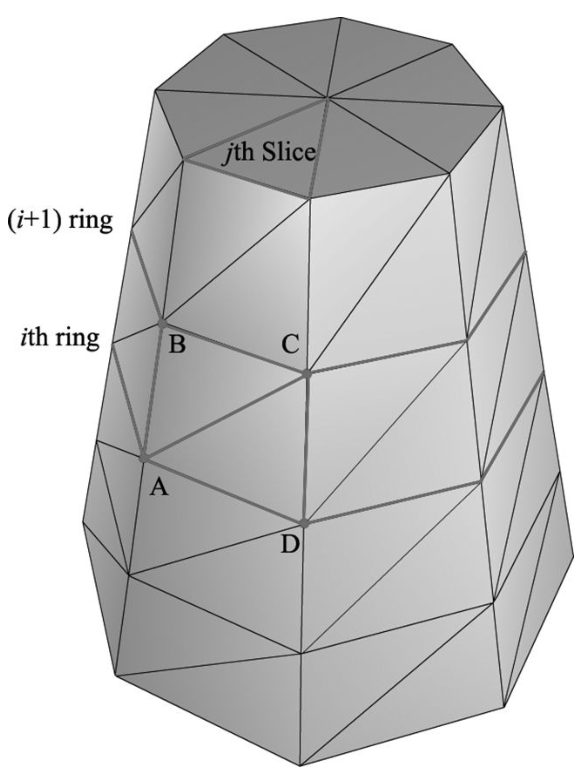
\includegraphics[width=\textwidth]{7-2}
    \centering
    \caption{包含在第$i$个和第$i + 1$个环中的顶点A,B,C,D和第$j$个切片。}
    \label{fig:7-2}
\end{figure}

%---- 7.4.1.2 ----
\subsubsection{顶面底面几何(Cap Geometry)}
\begin{flushleft}
生成顶面几何图形相当于生成顶部和底部环的切片三角形以近似圆形:\\
\end{flushleft}
\begin{lstlisting}
void GeometryGenerator::BuildCylinderTopCap(
    float bottomRadius, 
    float topRadius, 
    float height,
    uint32 sliceCount, 
    uint32 stackCount, 
    MeshData& meshData)
{
    uint32 baseIndex = (uint32)meshData.Vertices.size();

    float y = 0.5f*height;
    float dTheta = 2.0f*XM_PI/sliceCount;

    // Duplicate cap ring vertices because 
    // the texture coordinates and normals differ.
    for(uint32 i = 0; i <= sliceCount; ++i)
    {
        float x = topRadius*cosf(i*dTheta);
        float z = topRadius*sinf(i*dTheta);

        // Scale down by the height to try and 
        // make top cap texture coord area
        // proportional to base.
        float u = x/height + 0.5f;
        float v = z/height + 0.5f;

        meshData.Vertices.push_back(
            Vertex(x, y, z, 
                0.0f, 1.0f, 0.0f, 
                1.0f, 0.0f, 0.0f, 
                u, v));
    }

    // Cap center vertex.
    meshData.Vertices.push_back(
        Vertex(0.0f, y, 0.0f, 
            0.0f, 1.0f, 0.0f, 
            1.0f, 0.0f, 0.0f, 
            0.5f, 0.5f));

    // Index of center vertex.
    uint32 centerIndex = (uint32)meshData.Vertices.size()-1;

    for(uint32 i = 0; i < sliceCount; ++i)
    {
        meshData.Indices32.push_back(centerIndex);
        meshData.Indices32.push_back(baseIndex + i+1);
        meshData.Indices32.push_back(baseIndex + i);
    }
}
\end{lstlisting}
\begin{flushleft}
底面类似。\\
\end{flushleft}

%---- 7.4.2 ----
\subsection{创建球面网格(Generating a Sphere Mesh)}
\begin{flushleft}
我们通过指定半径,切片和堆栈计数来定义球体,如图\ref{fig:7-3}所示。 除了每个环的半径变化是基于三角函数的非线性方式之外,用于生成球体的算法非常类似于圆柱体的算法。 我们将留给读者研究 GeometryGenerator::CreateSphere 代码。 请注意,我们可以应用非均匀缩放世界变换将球体变换为椭圆体。
\end{flushleft}
\begin{figure}[h]
    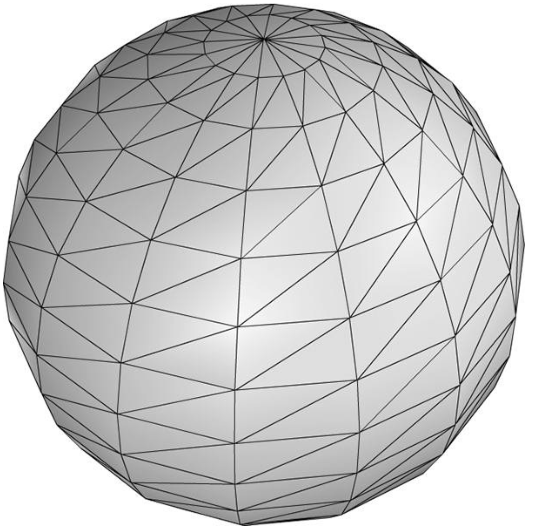
\includegraphics[width=\textwidth]{7-3}
    \centering
    \caption{切片和堆栈的思想也适用于球体来控制曲面细分的级别。}
    \label{fig:7-3}
\end{figure}

%---- 7.4.3 ----
\subsection{创建地圈网格(Generating a Geosphere Mesh)}
\begin{flushleft}
从图\ref{fig:7-3}可以看出,球体的三角形没有相等的面积。 在某些情况下这可能是不合需要的。 地圈使用具有几乎相等面积的三角形以及相等的边长来近似球体(参见图\ref{fig:7-4})。
\end{flushleft}

\begin{figure}[h]
    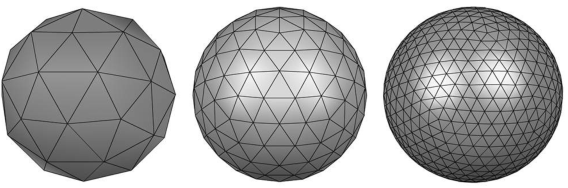
\includegraphics[width=\textwidth]{7-4}
    \centering
    \caption{通过重复细分和重投影到球体上来近似地圈。}
    \label{fig:7-4}
\end{figure}

\begin{flushleft}
为了生成地圈,我们从二十面体开始,细分三角形,然后将新顶点投影到具有给定半径的球体上。 我们可以重复此过程以改进曲面细分。\\
图\ref{fig:7-5}显示了如何将三角形细分为四个相等大小的三角形。 只需沿原始三角形的边缘取中点即可找到新的顶点。 然后,通过将顶点投影到单位球上然后标量乘以$r: v^{'}=r \frac{v}{||v||}$,可以将新顶点投影到半径为$r$的球体上
\end{flushleft}

\begin{figure}[h]
    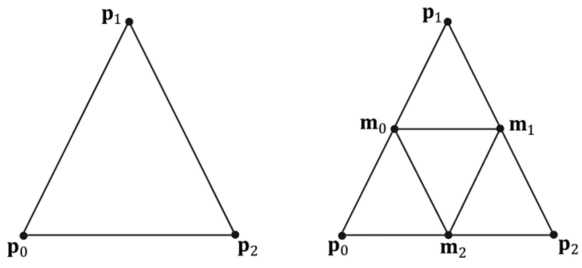
\includegraphics[width=\textwidth]{7-5}
    \centering
    \caption{将三角形细分为四个相等面积的三角形。}
    \label{fig:7-5}
\end{figure}

\begin{flushleft}
代码如下:\\
\end{flushleft}
\begin{lstlisting}
GeometryGenerator::MeshData 
GeometryGenerator::CreateGeosphere(
    float radius, 
    uint32 numSubdivisions)
{
    MeshData meshData;

    // Put a cap on the number of subdivisions.
    numSubdivisions = std::min<uint32>(numSubdivisions, 6u);

    // Approximate a sphere by tessellating an icosahedron.

    const float X = 0.525731f; 
    const float Z = 0.850651f;

    XMFLOAT3 pos[12] = 
    {
        XMFLOAT3(-X, 0.0f, Z),  XMFLOAT3(X, 0.0f, Z),  
        XMFLOAT3(-X, 0.0f, -Z), XMFLOAT3(X, 0.0f, -Z),    
        XMFLOAT3(0.0f, Z, X),   XMFLOAT3(0.0f, Z, -X), 
        XMFLOAT3(0.0f, -Z, X),  XMFLOAT3(0.0f, -Z, -X),    
        XMFLOAT3(Z, X, 0.0f),   XMFLOAT3(-Z, X, 0.0f), 
        XMFLOAT3(Z, -X, 0.0f),  XMFLOAT3(-Z, -X, 0.0f)
    };

    uint32 k[60] =
    {
        1,4,0,  4,9,0,  4,5,9,  8,5,4,  1,8,4,    
        1,10,8, 10,3,8, 8,3,5,  3,2,5,  3,7,2,    
        3,10,7, 10,6,7, 6,11,7, 6,0,11, 6,1,0, 
        10,1,6, 11,0,9, 2,11,9, 5,2,9,  11,2,7 
    };

    meshData.Vertices.resize(12);
    meshData.Indices32.assign(&k[0], &k[60]);

    for(uint32 i = 0; i < 12; ++i)
        meshData.Vertices[i].Position = pos[i];

    for(uint32 i = 0; i < numSubdivisions; ++i)
        Subdivide(meshData);

    // Project vertices onto sphere and scale.
    for(uint32 i = 0; i < meshData.Vertices.size(); ++i)
    {
        // Project onto unit sphere.
        XMVECTOR n = XMVector3Normalize(XMLoadFloat3(&meshData.Vertices[i].Position));

        // Project onto sphere.
        XMVECTOR p = radius*n;

        XMStoreFloat3(&meshData.Vertices[i].Position, p);
        XMStoreFloat3(&meshData.Vertices[i].Normal, n);

        // Derive texture coordinates from spherical coordinates.
        float theta = atan2f(meshData.Vertices[i].Position.z, 
                             meshData.Vertices[i].Position.x);

        // Put in [0, 2pi].
        if(theta < 0.0f)
            theta += XM_2PI;

        float phi = acosf(meshData.Vertices[i].Position.y / radius);

        meshData.Vertices[i].TexC.x = theta/XM_2PI;
        meshData.Vertices[i].TexC.y = phi/XM_PI;

        // Partial derivative of P with respect to theta
        meshData.Vertices[i].TangentU.x = -radius*sinf(phi)*sinf(theta);
        meshData.Vertices[i].TangentU.y = 0.0f;
        meshData.Vertices[i].TangentU.z = +radius*sinf(phi)*cosf(theta);

        XMVECTOR T = XMLoadFloat3(&meshData.Vertices[i].TangentU);
        XMStoreFloat3(&meshData.Vertices[i].TangentU, XMVector3Normalize(T));
    }

    return meshData;
}
\end{lstlisting}

%---- 7.5 ----
\section{Shapes Demo}
\begin{flushleft}
为了演示我们的球体和圆柱体生成代码,我们实现了如图\ref{fig:7-6}所示的 "Shapes" 演示。 此外,您还将获得在场景中定位和绘制多个对象的经验(即,创建多个世界变换矩阵)。 此外,我们将所有场景几何体放在一个大顶点和索引缓冲区中。 然后我们将使用 DrawIndexedInstanced 方法一次绘制一个对象(因为需要在对象之间更改世界矩阵); 因此,您将看到使用 DrawIndexedInstanced 的 StartIndexLocation 和 BaseVertexLocation 参数的示例。\\
\end{flushleft}

\begin{figure}[h]
    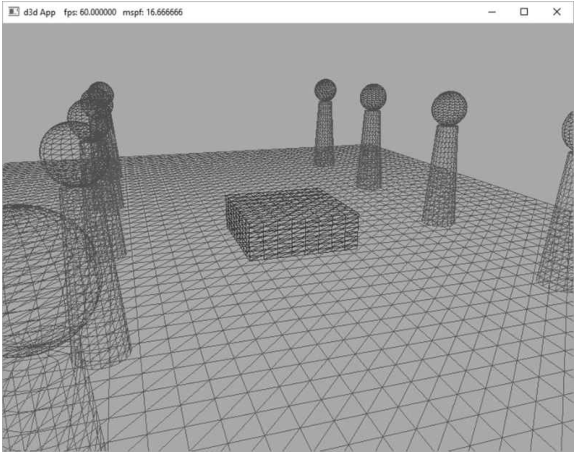
\includegraphics[width=\textwidth]{7-6}
    \centering
    \caption{"Shapes"演示的截图}
    \label{fig:7-6}
\end{figure}

%---- 7.5.1 ----
\subsection{顶点和顶点缓冲区(Vertex and Index Buffers)}
\begin{flushleft}
如图\ref{fig:7-6}所示,在本演示中,我们绘制了一个框,网格(grid),圆柱体和球体。 尽管我们在此演示中绘制了多个球体和圆柱体,但我们只需要一个球体和圆柱体几何体的副本。 我们只是多次重绘相同的球体和圆柱网格,但是使用不同的世界矩阵; 这是几何实例化的一个例子,它可以节省内存。\\
我们将所有网格顶点和索引打包到一个顶点和索引缓冲区中。 这是通过连接顶点和索引数组来完成的。 这意味着当我们绘制一个对象时,我们只绘制顶点和索引缓冲区的子集。 为了使用 ID3D12CommandList::DrawIndexedInstanced 仅绘制几何的子集,我们需要知道三个量(回想一下图\ref{fig:6-3}以及第6章中关于它的讨论)。 我们需要知道连接索引缓冲区中对象的起始索引,它的索引计数,我们需要知道基本顶点位置 - 对象相对于连接顶点缓冲区的第一个顶点的索引。 回想一下,基本顶点位置是在提取顶点之前添加到绘制调用中的索引的整数值,以便索引引用连接顶点缓冲区中的正确子集。 (另见第5章的练习2)\\

下面的代码显示了如何创建几何缓冲区,如何缓存必要的图纸数量以及如何绘制对象。
\end{flushleft}

\begin{lstlisting}
void ShapesApp::BuildShapeGeometry()
{
    GeometryGenerator geoGen;
    GeometryGenerator::MeshData box = 
        geoGen.CreateBox(1.5f, 0.5f, 1.5f, 3);
    GeometryGenerator::MeshData grid = 
        geoGen.CreateGrid(20.0f, 30.0f, 60, 40);
    GeometryGenerator::MeshData sphere = 
        geoGen.CreateSphere(0.5f, 20, 20);
    GeometryGenerator::MeshData cylinder = 
        geoGen.CreateCylinder(0.5f, 0.3f, 3.0f, 20, 20);

    //
    // We are concatenating all the geometry 
    // into one big vertex/index buffer.  So
    // define the regions in the buffer each submesh covers.
    //

    // Cache the vertex offsets to each object 
    // in the concatenated vertex buffer.
    UINT boxVertexOffset = 0;
    UINT gridVertexOffset = (UINT)box.Vertices.size();
    UINT sphereVertexOffset = gridVertexOffset + 
                           (UINT)grid.Vertices.size();
    UINT cylinderVertexOffset = sphereVertexOffset + 
                           (UINT)sphere.Vertices.size();

    // Cache the starting index for each object in the concatenated index buffer.
    UINT boxIndexOffset = 0;
    UINT gridIndexOffset = (UINT)box.Indices32.size();
    UINT sphereIndexOffset = gridIndexOffset + 
                           (UINT)grid.Indices32.size();
    UINT cylinderIndexOffset = sphereIndexOffset + 
                           (UINT)sphere.Indices32.size();

    // Define the SubmeshGeometry that cover different 
    // regions of the vertex/index buffers.

    SubmeshGeometry boxSubmesh;
    boxSubmesh.IndexCount = (UINT)box.Indices32.size();
    boxSubmesh.StartIndexLocation = boxIndexOffset;
    boxSubmesh.BaseVertexLocation = boxVertexOffset;

    SubmeshGeometry gridSubmesh;
    gridSubmesh.IndexCount = (UINT)grid.Indices32.size();
    gridSubmesh.StartIndexLocation = gridIndexOffset;
    gridSubmesh.BaseVertexLocation = gridVertexOffset;

    SubmeshGeometry sphereSubmesh;
    sphereSubmesh.IndexCount = (UINT)sphere.Indices32.size();
    sphereSubmesh.StartIndexLocation = sphereIndexOffset;
    sphereSubmesh.BaseVertexLocation = sphereVertexOffset;

    SubmeshGeometry cylinderSubmesh;
    cylinderSubmesh.IndexCount = (UINT)cylinder.Indices32.size();
    cylinderSubmesh.StartIndexLocation = cylinderIndexOffset;
    cylinderSubmesh.BaseVertexLocation = cylinderVertexOffset;

    //
    // Extract the vertex elements we are 
    // interested in and pack the
    // vertices of all the meshes into 
    // one vertex buffer.
    //

    auto totalVertexCount =
        box.Vertices.size() +
        grid.Vertices.size() +
        sphere.Vertices.size() +
        cylinder.Vertices.size();

    std::vector<Vertex> vertices(totalVertexCount);

    UINT k = 0;
    for(size_t i = 0; i < box.Vertices.size(); ++i, ++k)
    {
        vertices[k].Pos = box.Vertices[i].Position;
        vertices[k].Color = XMFLOAT4(DirectX::Colors::DarkGreen);
    }

    for(size_t i = 0; i < grid.Vertices.size(); ++i, ++k)
    {
        vertices[k].Pos = grid.Vertices[i].Position;
        vertices[k].Color = XMFLOAT4(DirectX::Colors::ForestGreen);
    }

    for(size_t i = 0; i < sphere.Vertices.size(); ++i, ++k)
    {
        vertices[k].Pos = sphere.Vertices[i].Position;
        vertices[k].Color = XMFLOAT4(DirectX::Colors::Crimson);
    }

    for(size_t i = 0; i < cylinder.Vertices.size(); ++i, ++k)
    {
        vertices[k].Pos = cylinder.Vertices[i].Position;
        vertices[k].Color = XMFLOAT4(DirectX::Colors::SteelBlue);
    }

    std::vector<std::uint16_t> indices;
    indices.insert(indices.end(), 
                   std::begin(box.GetIndices16()), 
                   std::end(box.GetIndices16()));
    indices.insert(indices.end(), 
                   std::begin(grid.GetIndices16()), 
                   std::end(grid.GetIndices16()));
    indices.insert(indices.end(), 
                   std::begin(sphere.GetIndices16()), 
                   std::end(sphere.GetIndices16()));
    indices.insert(indices.end(), 
                   std::begin(cylinder.GetIndices16()), 
                   std::end(cylinder.GetIndices16()));

    const UINT vbByteSize = (UINT)vertices.size() * 
                            sizeof(Vertex);
    const UINT ibByteSize = (UINT)indices.size() * 
                            sizeof(std::uint16_t);

    auto geo = std::make_unique<MeshGeometry>();
    geo->Name = "shapeGeo";

    ThrowIfFailed(D3DCreateBlob(vbByteSize, &geo->VertexBufferCPU));
    CopyMemory(geo->VertexBufferCPU->GetBufferPointer(), 
                    vertices.data(), 
                    vbByteSize);

    ThrowIfFailed(D3DCreateBlob(ibByteSize, &geo->IndexBufferCPU));
    CopyMemory(geo->IndexBufferCPU->GetBufferPointer(), 
                    indices.data(), 
                    ibByteSize);

    geo->VertexBufferGPU = d3dUtil::CreateDefaultBuffer(md3dDevice.Get(),
        mCommandList.Get(), vertices.data(), 
        vbByteSize, geo->VertexBufferUploader);

    geo->IndexBufferGPU = d3dUtil::CreateDefaultBuffer(md3dDevice.Get(),
        mCommandList.Get(), indices.data(), 
        ibByteSize, geo->IndexBufferUploader);

    geo->VertexByteStride = sizeof(Vertex);
    geo->VertexBufferByteSize = vbByteSize;
    geo->IndexFormat = DXGI_FORMAT_R16_UINT;
    geo->IndexBufferByteSize = ibByteSize;

    geo->DrawArgs["box"] = boxSubmesh;
    geo->DrawArgs["grid"] = gridSubmesh;
    geo->DrawArgs["sphere"] = sphereSubmesh;
    geo->DrawArgs["cylinder"] = cylinderSubmesh;

    mGeometries[geo->Name] = std::move(geo);
}
\end{lstlisting}

\begin{flushleft}
在上面方法的最后一行中使用的 mGeometries 变量定义如下:\\
\end{flushleft}

\begin{lstlisting}
std::unordered_map<std::string, 
            std::unique_ptr<MeshGeometry>> mGeometries;
\end{lstlisting}

\begin{flushleft}
这是我们在本书其余部分使用的常见模式。 为每个几何体,PSO,纹理,着色器等创建新的变量名称很麻烦,因此我们使用无序地图进行常量时间查找并按名称引用我们的对象。 以下是一些例子:\\
\end{flushleft}

\begin{lstlisting}
std::unordered_map<std::string,
    std::unique_ptr<MeshGeometry>> mGeometries;
std::unordered_map<std::string, ComPtr<ID3DBlob>>
    mShaders;
std::unordered_map<std::string,
    ComPtr<ID3D12PipelineState>> mPSOs;
\end{lstlisting}

%---- 7.5.2 ----
\subsection{渲染项(Render Items)}
\begin{flushleft}
我们现在定义场景渲染项。 观察所有渲染项如何共享相同的 MeshGeometry,并使用 DrawArgs 获取 DrawIndexedInstanced 参数以绘制顶点/索引缓冲区的子区域。\\
\end{flushleft}

\begin{lstlisting}
// ShapesApp member variable.
std::vector<std::unique_ptr<RenderItem>> mAllRitems;
std::vector<RenderItem*> mOpaqueRitems;

void ShapesApp::BuildRenderItems()
{
    auto boxRitem = std::make_unique<RenderItem>();
    XMStoreFloat4x4(&boxRitem->World, 
         XMMatrixScaling(2.0f, 2.0f, 2.0f)*
         XMMatrixTranslation(0.0f, 0.5f, 0.0f));

    boxRitem->ObjCBIndex = 0;
    boxRitem->Geo = mGeometries["shapeGeo"].get();
    boxRitem->PrimitiveType = D3D_PRIMITIVE_TOPOLOGY_TRIANGLELIST;
    boxRitem->IndexCount = boxRitem->Geo->
        DrawArgs["box"].IndexCount;
    boxRitem->StartIndexLocation = boxRitem->Geo->
        DrawArgs["box"].StartIndexLocation;
    boxRitem->BaseVertexLocation = boxRitem->Geo->
        DrawArgs["box"].BaseVertexLocation;
    mAllRitems.push_back(std::move(boxRitem));

    auto gridRitem = std::make_unique<RenderItem>();
    gridRitem->World = MathHelper::Identity4x4();
    gridRitem->ObjCBIndex = 1;
    gridRitem->Geo = mGeometries["shapeGeo"].get();
    gridRitem->PrimitiveType = D3D_PRIMITIVE_TOPOLOGY_TRIANGLELIST;
    gridRitem->IndexCount = gridRitem->Geo->
        DrawArgs["grid"].IndexCount;
    gridRitem->StartIndexLocation = gridRitem->Geo->
        DrawArgs["grid"].StartIndexLocation;
    gridRitem->BaseVertexLocation = gridRitem->Geo->
        DrawArgs["grid"].BaseVertexLocation;
    mAllRitems.push_back(std::move(gridRitem));

    UINT objCBIndex = 2;
    for(int i = 0; i < 5; ++i)
    {
        auto leftCylRitem = std::make_unique<RenderItem>();
        auto rightCylRitem = std::make_unique<RenderItem>();
        auto leftSphereRitem = std::make_unique<RenderItem>();
        auto rightSphereRitem = std::make_unique<RenderItem>();

        XMMATRIX leftCylWorld = XMMatrixTranslation(
            -5.0f, 1.5f, -10.0f + i*5.0f);
        XMMATRIX rightCylWorld = XMMatrixTranslation(
            +5.0f, 1.5f, -10.0f + i*5.0f);

        XMMATRIX leftSphereWorld = XMMatrixTranslation(
            -5.0f, 3.5f, -10.0f + i*5.0f);
        XMMATRIX rightSphereWorld = XMMatrixTranslation(
            +5.0f, 3.5f, -10.0f + i*5.0f);

        XMStoreFloat4x4(&leftCylRitem->World, 
            rightCylWorld);
        leftCylRitem->ObjCBIndex = objCBIndex++;
        leftCylRitem->Geo = mGeometries["shapeGeo"].get();
        leftCylRitem->PrimitiveType = 
            D3D_PRIMITIVE_TOPOLOGY_TRIANGLELIST;
        leftCylRitem->IndexCount = leftCylRitem->Geo->
            DrawArgs["cylinder"].IndexCount;
        leftCylRitem->StartIndexLocation = leftCylRitem->Geo->
            DrawArgs["cylinder"].StartIndexLocation;
        leftCylRitem->BaseVertexLocation = leftCylRitem->Geo->
            DrawArgs["cylinder"].BaseVertexLocation;

        XMStoreFloat4x4(&rightCylRitem->World, leftCylWorld);
        rightCylRitem->ObjCBIndex = objCBIndex++;
        rightCylRitem->Geo = mGeometries["shapeGeo"].get();
        rightCylRitem->PrimitiveType = 
            D3D_PRIMITIVE_TOPOLOGY_TRIANGLELIST;
        rightCylRitem->IndexCount = rightCylRitem->Geo->
            DrawArgs["cylinder"].IndexCount;
        rightCylRitem->StartIndexLocation = rightCylRitem->Geo->
            DrawArgs["cylinder"].StartIndexLocation;
        rightCylRitem->BaseVertexLocation = rightCylRitem->Geo->
            DrawArgs["cylinder"].BaseVertexLocation;

        XMStoreFloat4x4(&leftSphereRitem->World, leftSphereWorld);
        leftSphereRitem->ObjCBIndex = objCBIndex++;
        leftSphereRitem->Geo = mGeometries["shapeGeo"].get();
        leftSphereRitem->PrimitiveType = 
            D3D_PRIMITIVE_TOPOLOGY_TRIANGLELIST;
        leftSphereRitem->IndexCount = leftSphereRitem->Geo->
            DrawArgs["sphere"].IndexCount;
        leftSphereRitem->StartIndexLocation = leftSphereRitem->Geo->
            DrawArgs["sphere"].StartIndexLocation;
        leftSphereRitem->BaseVertexLocation = leftSphereRitem->Geo->
            DrawArgs["sphere"].BaseVertexLocation;

        XMStoreFloat4x4(&rightSphereRitem->World, rightSphereWorld);
        rightSphereRitem->ObjCBIndex = objCBIndex++;
        rightSphereRitem->Geo = mGeometries["shapeGeo"].get();
        rightSphereRitem->PrimitiveType = 
            D3D_PRIMITIVE_TOPOLOGY_TRIANGLELIST;
        rightSphereRitem->IndexCount = rightSphereRitem->Geo->
            DrawArgs["sphere"].IndexCount;
        rightSphereRitem->StartIndexLocation = rightSphereRitem->Geo->
            DrawArgs["sphere"].StartIndexLocation;
        rightSphereRitem->BaseVertexLocation = rightSphereRitem->Geo->
            DrawArgs["sphere"].BaseVertexLocation;

        mAllRitems.push_back(std::move(leftCylRitem));
        mAllRitems.push_back(std::move(rightCylRitem));
        mAllRitems.push_back(std::move(leftSphereRitem));
        mAllRitems.push_back(std::move(rightSphereRitem));
    }

    // All the render items are opaque.
    for(auto& e : mAllRitems)
        mOpaqueRitems.push_back(e.get());
}
\end{lstlisting}

%---- 7.5.3 ----
\subsection{帧资源和常量缓冲视图(Frame Resources and Constant Buffer Views)}
\begin{flushleft}
回想一下,我们有一个 FrameResources 的向量,每个 FrameResource 都有一个上传缓冲区,用于存储场景中每个渲染项的传递常量和常量缓冲区。
\end{flushleft}

\begin{lstlisting}
std::unique_ptr<UploadBuffer<PassConstants>> PassCB = nullptr;
std::unique_ptr<UploadBuffer<ObjectConstants>> ObjectCB = nullptr;
\end{lstlisting}

\begin{flushleft}
如果我们有3个帧资源和 $n$ 个渲染项,那么我们有 $3n$ 个对象\footnote{原文是:"then we have three 3n object constant
buffers",是错误的}常量缓冲区和3个传递常量缓冲区。 因此,我们需要$3(n+1)$个常量缓冲区视图(CBV)。 所以,我们需要修改我们的CBV堆以包含其他描述符:\\
\end{flushleft}

\begin{lstlisting}
void ShapesApp::BuildDescriptorHeaps()
{
    UINT objCount = (UINT)mOpaqueRitems.size();

    // Need a CBV descriptor for each object for each frame resource,
    // +1 for the perPass CBV for each frame resource.
    UINT numDescriptors = (objCount+1) * 3;

    // Save an offset to the start of the pass CBVs.  
    // These are the last 3 descriptors.
    mPassCbvOffset = objCount * gNumFrameResources;

    D3D12_DESCRIPTOR_HEAP_DESC cbvHeapDesc;
    cbvHeapDesc.NumDescriptors = numDescriptors;
    cbvHeapDesc.Type = D3D12_DESCRIPTOR_HEAP_TYPE_CBV_SRV_UAV;
    cbvHeapDesc.Flags = D3D12_DESCRIPTOR_HEAP_FLAG_SHADER_VISIBLE;
    cbvHeapDesc.NodeMask = 0;
    ThrowIfFailed(md3dDevice->CreateDescriptorHeap(&cbvHeapDesc,
        IID_PPV_ARGS(&mCbvHeap)));
}
\end{lstlisting}

\begin{flushleft}
现在,我们可以使用以下代码填充CBV堆,其中描述符$0$到$n-1$包含第$0$帧资源的对象CBV,描述符$n$到$2n-1$包含第$1$帧资源的对象CBV,描述符$2n$到$3n-1$ 包含第二帧资源的对象CBV,描述符$3n$,$3n + 1$和$3n + 2$分别包含第$0$帧,第$1$帧和第$2$帧资源的传递CBV:\\
\end{flushleft}

\begin{lstlisting}
void ShapesApp::BuildConstantBufferViews()
{
    UINT objCBByteSize = d3dUtil::CalcConstantBufferByteSize(
            sizeof(ObjectConstants));

    UINT objCount = (UINT)mOpaqueRitems.size();

    // Need a CBV descriptor for each object for each frame resource.
    for(int frameIndex = 0; 
        frameIndex < gNumFrameResources; 
        ++frameIndex)
    {
        auto objectCB = mFrameResources[frameIndex]->
            ObjectCB->Resource();
        for(UINT i = 0; i < objCount; ++i)
        {
            D3D12_GPU_VIRTUAL_ADDRESS cbAddress = 
                objectCB->GetGPUVirtualAddress();

            // Offset to the ith object constant buffer in the buffer.
            cbAddress += i*objCBByteSize;

            // Offset to the object cbv in the descriptor heap.
            int heapIndex = frameIndex*objCount + i;
            auto handle = CD3DX12_CPU_DESCRIPTOR_HANDLE(mCbvHeap->
                GetCPUDescriptorHandleForHeapStart());
            handle.Offset(heapIndex, mCbvSrvUavDescriptorSize);

            D3D12_CONSTANT_BUFFER_VIEW_DESC cbvDesc;
            cbvDesc.BufferLocation = cbAddress;
            cbvDesc.SizeInBytes = objCBByteSize;

            md3dDevice->CreateConstantBufferView(&cbvDesc, handle);
        }
    }

    UINT passCBByteSize = d3dUtil::CalcConstantBufferByteSize(
        sizeof(PassConstants));

    // Last three descriptors are the pass CBVs for each frame resource.
    for(int frameIndex = 0; frameIndex < gNumFrameResources; ++frameIndex)
    {
        auto passCB = mFrameResources[frameIndex]->PassCB->Resource();
        D3D12_GPU_VIRTUAL_ADDRESS cbAddress = passCB->GetGPUVirtualAddress();

        // Offset to the pass cbv in the descriptor heap.
        int heapIndex = mPassCbvOffset + frameIndex;
        auto handle = CD3DX12_CPU_DESCRIPTOR_HANDLE(mCbvHeap->
            GetCPUDescriptorHandleForHeapStart());
        handle.Offset(heapIndex, mCbvSrvUavDescriptorSize);

        D3D12_CONSTANT_BUFFER_VIEW_DESC cbvDesc;
        cbvDesc.BufferLocation = cbAddress;
        cbvDesc.SizeInBytes = passCBByteSize;
        
        md3dDevice->CreateConstantBufferView(&cbvDesc, handle);
    }
}
\end{lstlisting}

\begin{flushleft}
回想一下,我们可以使用 ID3D12DescriptorHeap::GetCPUDescriptorHandleForHeapStart 方法获取堆中第一个描述符的句柄。 但是,现在我们的堆有多个描述符,这个方法已不再适用。 我们需要能够偏移到堆中的其他描述符。 为此,我们需要知道要在堆中递增的大小以获取到下一个描述符。 这是特定于硬件的,因此我们必须从设备查询此信息,这取决于堆类型。 回想一下,我们的 D3DApp 类缓存了这些信息:\\
\end{flushleft}

\begin{lstlisting}
mRtvDescriptorSize = md3dDevice->
    GetDescriptorHandleIncrementSize(
    D3D12_DESCRIPTOR_HEAP_TYPE_RTV);
mDsvDescriptorSize = md3dDevice->
    GetDescriptorHandleIncrementSize(
    D3D12_DESCRIPTOR_HEAP_TYPE_DSV);
mCbvSrvUavDescriptorSize = md3dDevice->
    GetDescriptorHandleIncrementSize(
    D3D12_DESCRIPTOR_HEAP_TYPE_CBV_SRV_UAV);
\end{lstlisting}

\begin{flushleft}
一旦我们知道描述符增量大小,我们就可以使用两个 CD3DX12\_CPU\_DESCRIPTOR\_HANDLE::Offset 方法之一来通过 n 个描述符来偏移句柄:\\
\end{flushleft}

\begin{lstlisting}
// Specify the number of descriptors to offset times 
// the descriptor Offset by n descriptors:
CD3DX12_CPU_DESCRIPTOR_HANDLE handle = mCbvHeap->
    GetCPUDescriptorHandleForHeapStart();
handle.Offset(n * mCbvSrvDescriptorSize);

// Or equivalently, specify the number of 
// descriptors to offset, followed by 
// the descriptor increment size:
CD3DX12_CPU_DESCRIPTOR_HANDLE handle = mCbvHeap->
    GetCPUDescriptorHandleForHeapStart();
handle.Offset(n, mCbvSrvDescriptorSize);
\end{lstlisting}

\begin{flushleft}
NOTICE: CD3DX12\_GPU\_DESCRIPTOR\_HANDLE 有相同的 Offset 方法。
\end{flushleft}


%---- 7.5.4 ----
\subsection{绘制场景(Draw the Scene)}
\begin{flushleft}
最后我们可以绘制渲染项。 也许唯一棘手的部分是通过程序偏移到堆中(我们想要绘制的对象的)正确CBV。 注意渲染项如何将索引存储到与渲染项关联的常量缓冲区的。\\
\end{flushleft}

\begin{lstlisting}
void ShapesApp::DrawRenderItems(
    ID3D12GraphicsCommandList* cmdList, 
    const std::vector<RenderItem*>& ritems)
{
    UINT objCBByteSize = d3dUtil::CalcConstantBufferByteSize(
        sizeof(ObjectConstants));
 
    auto objectCB = mCurrFrameResource->ObjectCB->Resource();

    // For each render item...
    for(size_t i = 0; i < ritems.size(); ++i)
    {
        auto ri = ritems[i];

        cmdList->IASetVertexBuffers(0, 1, 
            &ri->Geo->VertexBufferView());
        cmdList->IASetIndexBuffer(
            &ri->Geo->IndexBufferView());
        cmdList->IASetPrimitiveTopology(
            ri->PrimitiveType);

        // Offset to the CBV in the descriptor heap for 
        // this object and for this frame resource.
        UINT cbvIndex = mCurrFrameResourceIndex*
            (UINT)mOpaqueRitems.size() + ri->ObjCBIndex;
        auto cbvHandle = CD3DX12_GPU_DESCRIPTOR_HANDLE(mCbvHeap->
            GetGPUDescriptorHandleForHeapStart());
        cbvHandle.Offset(cbvIndex, mCbvSrvUavDescriptorSize);

        cmdList->SetGraphicsRootDescriptorTable(0, cbvHandle);

        cmdList->DrawIndexedInstanced(ri->IndexCount, 1, 
            ri->StartIndexLocation, ri->BaseVertexLocation, 0);
    }
}
\end{lstlisting}

\begin{flushleft}
DrawRenderItems 方法由 Draw 调用:\\
\end{flushleft}

\begin{lstlisting}
void ShapesApp::Draw(const GameTimer& gt)
{
    auto cmdListAlloc = mCurrFrameResource->CmdListAlloc;

    // Reuse the memory associated with command recording.
    // We can only reset when the associated command 
    // lists have finished execution on the GPU.
    ThrowIfFailed(cmdListAlloc->Reset());

    // A command list can be reset after it has 
    // been added to the command queue via ExecuteCommandList.
    // Reusing the command list reuses memory.
    if(mIsWireframe)
    {
        ThrowIfFailed(mCommandList->Reset(
            cmdListAlloc.Get(), 
            mPSOs["opaque_wireframe"].Get()));
    }
    else
    {
        ThrowIfFailed(mCommandList->Reset(
            cmdListAlloc.Get(), 
            mPSOs["opaque"].Get()));
    }

    mCommandList->RSSetViewports(1, &mScreenViewport);
    mCommandList->RSSetScissorRects(1, &mScissorRect);

    // Indicate a state transition on the resource usage.
    mCommandList->ResourceBarrier(1, 
        &CD3DX12_RESOURCE_BARRIER::Transition(
            CurrentBackBuffer(),
            D3D12_RESOURCE_STATE_PRESENT, 
            D3D12_RESOURCE_STATE_RENDER_TARGET));

    // Clear the back buffer and depth buffer.
    mCommandList->ClearRenderTargetView(CurrentBackBufferView(), 
        Colors::LightSteelBlue, 0, nullptr);
    mCommandList->ClearDepthStencilView(DepthStencilView(), 
        D3D12_CLEAR_FLAG_DEPTH | D3D12_CLEAR_FLAG_STENCIL, 
        1.0f, 0, 0, nullptr);

    // Specify the buffers we are going to render to.
    mCommandList->OMSetRenderTargets(1, &CurrentBackBufferView(), 
        true, &DepthStencilView());

    ID3D12DescriptorHeap* descriptorHeaps[] = { mCbvHeap.Get() };
    mCommandList->SetDescriptorHeaps(
        _countof(descriptorHeaps), 
        descriptorHeaps);

	mCommandList->SetGraphicsRootSignature(mRootSignature.Get());

    int passCbvIndex = mPassCbvOffset + mCurrFrameResourceIndex;
    auto passCbvHandle = CD3DX12_GPU_DESCRIPTOR_HANDLE(
        mCbvHeap->GetGPUDescriptorHandleForHeapStart());
    passCbvHandle.Offset(passCbvIndex, mCbvSrvUavDescriptorSize);
    mCommandList->SetGraphicsRootDescriptorTable(1, passCbvHandle);

    DrawRenderItems(mCommandList.Get(), mOpaqueRitems);

    // Indicate a state transition on the resource usage.
    mCommandList->ResourceBarrier(1, 
        &CD3DX12_RESOURCE_BARRIER::Transition(
            CurrentBackBuffer(),
            D3D12_RESOURCE_STATE_RENDER_TARGET, 
            D3D12_RESOURCE_STATE_PRESENT));

    // Done recording commands.
    ThrowIfFailed(mCommandList->Close());

    // Add the command list to the queue for execution.
    ID3D12CommandList* cmdsLists[] = { mCommandList.Get() };
    mCommandQueue->ExecuteCommandLists(_countof(cmdsLists), cmdsLists);

    // Swap the back and front buffers
    ThrowIfFailed(mSwapChain->Present(0, 0));
    mCurrBackBuffer = (mCurrBackBuffer + 1) % SwapChainBufferCount;

    // Advance the fence value to mark commands 
    // up to this fence point.
    mCurrFrameResource->Fence = ++mCurrentFence;
    
    // Add an instruction to the command queue 
    // to set a new fence point. 
    // Because we are on the GPU timeline, 
    // the new fence point won't be 
    // set until the GPU finishes processing all
    // the commands prior to this Signal().
    mCommandQueue->Signal(mFence.Get(), mCurrentFence);
}
\end{lstlisting}

%---- 7.6 ----
\section{更多关于根签名(More on Root Signatures)}
\begin{flushleft}
我们在前一章的第6.6.5节中介绍了根签名。 根签名定义在发出绘制调用之前需要将哪些资源绑定到管道以及这些资源如何映射到着色器输入寄存器。 需要绑定哪些资源取决于当前着色器程序所期望的资源。 创建PSO时,将验证根签名和着色器程序组合。
\end{flushleft}

%---- 7.6.1 ----
\subsection{根参数(Root Parameters)}
\begin{flushleft}
回想一下,根签名是由一组根参数定义的。 到目前为止,我们只创建了一个存储描述符表的根参数。 但是,root参数实际上可以是以下三种类型之一:\\
\end{flushleft}

\begin{itemize}
  \item 描述符表(Descriptor Table): 期望描述符表引用堆中的连续范围,该范围标识要绑定的资源。
  \item 根描述符(Root Descriptor | Inline Descriptor): 期望直接设置描述符以识别要绑定的资源; 描述符不需要在堆中。 只有 CBV 到常量缓冲区,SRV/UAV 到缓冲区可以绑定为根描述符。 特别是,这意味着 SRV 到纹理不能绑定为根描述符。
  \item 根常量(Root constant): 期望直接绑定的32位常量值列表。
\end{itemize}

\begin{flushleft}
出于性能考虑,可以将64个DWORD限制在根签名中。 这三种根参数具有以下内存消耗:\\
\end{flushleft}

\begin{itemize}
  \item 描述符表(Descriptor Table): 1 DWORD
  \item 根描述符(Root Descriptor): 2 DWORDs
  \item 根常量(Root constant): 每 32-bit 常量 1 DWORD
\end{itemize}

\begin{flushleft}
我们可以创建一个任意的根签名,只要我们不超过64个DWORD限制。 根常量非常方便,但它们的成本很快就会增加。 例如,如果我们需要的唯一常量数据是世界视图投影矩阵,我们可以使用16个根常量来存储它,这将使我们不需要涉及常量缓冲区和CBV堆。 但是,这会占我们根签名预算的四分之一。 使用根描述符只能是两个DWORD,描述符表只有一个DWORD。 随着我们的应用程序变得越来越复杂,我们的常量缓冲区数据将变得越来越大,并且我们不太可能只使用根常量。 在实际应用程序中,您可能会使用所有三种类型的根参数的组合。\\
在代码中,通过填写 CD3DX12\_ROOT\_PARAMETER 结构来描述根参数。 正如我们在 CD3DX 代码中看到的那样,CD3DX12\_ROOT\_PARAMETER 扩展了 D3D12\_ROOT\_PARAMETER 并添加了一些辅助初始化函数。\\
\end{flushleft}

\begin{lstlisting}
typedef struct D3D12_ROOT_PARAMETER
{
    D3D12_ROOT_PARAMETER_TYPE ParameterType;
    union
    {
        D3D12_ROOT_DESCRIPTOR_TABLE DescriptorTable;
        D3D12_ROOT_CONSTANTS Constants;
        D3D12_ROOT_DESCRIPTOR Descriptor;
    };
    D3D12_SHADER_VISIBILITY ShaderVisibility;
} D3D12_ROOT_PARAMETER;
\end{lstlisting}

\begin{itemize}
  \item 1.ParameterType: 以下枚举类型的成员,指示根参数类型(描述符表,根常量,CBV根描述符,SRV根描述符,UAV根描述符)。
  \begin{lstlisting}
    enum D3D12_ROOT_PARAMETER_TYPE
    {
        D3D12_ROOT_PARAMETER_TYPE_DESCRIPTOR_TABLE = 0,
        D3D12_ROOT_PARAMETER_TYPE_32BIT_CONSTANTS = 1,
        D3D12_ROOT_PARAMETER_TYPE_CBV = 2,
        D3D12_ROOT_PARAMETER_TYPE_SRV = 3 ,
        D3D12_ROOT_PARAMETER_TYPE_UAV = 4
    } D3D12_ROOT_PARAMETER_TYPE;
  \end{lstlisting}
  \item 2.DescriptorTable/Constants/Descriptor: 描述根参数的结构。您填写的联合成员取决于根参数类型。 7.6.2节,7.6.3节和7.6.4节讨论了这些结构。
  \item 3.ShaderVisibility: 以下枚举的成员,指定哪个着色器程序可以看到此根参数。 通常在本书中我们指定 D3D12\_SHADER\_VISIBILITY\_ALL。 但是,如果我们知道资源仅用于像素着色器,那么我们可以指定 D3D12\_SHADER\_VISIBILITY\_PIXEL。 限制根参数的可见性可能会促使一些优化。\\
  \begin{lstlisting}
    enum D3D12_SHADER_VISIBILITY
    {
        D3D12_SHADER_VISIBILITY_ALL = 0,
        D3D12_SHADER_VISIBILITY_VERTEX = 1,
        D3D12_SHADER_VISIBILITY_HULL = 2,
        D3D12_SHADER_VISIBILITY_DOMAIN = 3,
        D3D12_SHADER_VISIBILITY_GEOMETRY = 4,
        D3D12_SHADER_VISIBILITY_PIXEL = 5
    } D3D12_SHADER_VISIBILITY;
  \end{lstlisting}
\end{itemize}

%---- 7.6.2 ----
\subsection{描述符表(Descriptor Tables)}
\begin{flushleft}
通过填写 D3D12\_ROOT\_PARAMETER 的 DescriptorTable 成员来进一步定义描述符表根参数。\\
\end{flushleft}

\begin{lstlisting}
typedef struct D3D12_ROOT_DESCRIPTOR_TABLE
{
    UINT NumDescriptorRanges;
    const D3D12_DESCRIPTOR_RANGE *pDescriptorRanges;
} D3D12_ROOT_DESCRIPTOR_TABLE;
\end{lstlisting}

\begin{flushleft}
这只是指定 D3D12\_DESCRIPTOR\_RANGE 的数组和数组中的范围数。\\
D3D12\_DESCRIPTOR\_RANGE 结构定义如下:\\
\end{flushleft}

\begin{lstlisting}
typedef struct D3D12_DESCRIPTOR_RANGE
{
    D3D12_DESCRIPTOR_RANGE_TYPE RangeType;
    UINT NumDescriptors;
    UINT BaseShaderRegister;
    UINT RegisterSpace;
    UINT OffsetInDescriptorsFromTableStart;
} D3D12_DESCRIPTOR_RANGE;
\end{lstlisting}

\begin{itemize}
  \item 1.RangeType: 以下枚举类型的成员,指示此范围中的描述符类型:\\
  \begin{lstlisting}
    enum D3D12_DESCRIPTOR_RANGE_TYPE
    {
    D3D12_DESCRIPTOR_RANGE_TYPE_SRV = 0,
    D3D12_DESCRIPTOR_RANGE_TYPE_UAV = 1,
    D3D12_DESCRIPTOR_RANGE_TYPE_CBV = 2 ,
    D3D12_DESCRIPTOR_RANGE_TYPE_SAMPLER = 3
    } D3D12_DESCRIPTOR_RANGE_TYPE;
  \end{lstlisting}
  NOTICE: 采样器描述符在纹理章节中讨论。
  \item 2.NumDescriptors: 范围中的描述符个数
  \item 3.BaseShaderRegister: 基本着色器寄存器参数绑定到。 例如,如果将 NumDescriptors 设置为3,将 BaseShaderRegister 设置为 1,范围类型为 CBV(对于常量缓冲区),那么您将绑定到 HLSL 寄存器\\
  \begin{lstlisting}
    cbuffer cbA : register(b1) {…};
    cbuffer cbB : register(b2) {…};
    cbuffer cbC : register(b3) {…};
  \end{lstlisting}
  \item 4.RegisterSpace: 此属性为您提供另一个指定着色器寄存器的维度。 例如,以下两个寄存器似乎与寄存器槽t0重叠,但它们是不同的寄存器,因为它们位于不同的空间中:\\
  \begin{lstlisting}
    Texture2D gDiffuseMap :register(t0,space0);
    Texture2D gNormalMap : register(t0, space1);
  \end{lstlisting}
  \item 5.OffsetInDescriptorsFromTableStart: 从表的开头偏移此范围的描述符。请参阅下面的示例。
\end{itemize}

\begin{flushleft}
初始化为描述符表的槽参数采用 D3D12\_DESCRIPTOR\_RANGE 实例的数组,因为我们可以在一个表中混合各种类型的描述符。 假设我们按顺序通过以下三个范围定义了六个描述符的表:两个CBV,三个SRV和一个UAV。 这个表的定义如下:\\
\end{flushleft}

\begin{lstlisting}
// Create a table with 2 CBVs, 3 SRVs and 1 UAV.
CD3DX12_DESCRIPTOR_RANGE descRange[3];
descRange[0].Init(
    D3D12_DESCRIPTOR_RANGE_TYPE_CBV, // descriptor type
    2, // descriptor count
    0, // base shader register arguments are bound to 
       // for this root parameter
    0, // register space
    0);// offset from start of table

descRange[1].Init(
    D3D12_DESCRIPTOR_RANGE_TYPE_SRV, // descriptor type
    3, // descriptor count
    0, // base shader register arguments are bound to 
       // for this root parameter
    0, // register space
    2);// offset from start of table
descRange[2].Init(
    D3D12_DESCRIPTOR_RANGE_TYPE_UAV, // descriptor type
    1, // descriptor count
    0, // base shader register arguments are bound to 
       // for this root parameter
    0, // register space
    5);// offset from start of table
slotRootParameter[0].InitAsDescriptorTable(
    3, descRange, D3D12_SHADER_VISIBILITY_ALL);
\end{lstlisting}

\begin{flushleft}
像往常一样,有一个继承自 D3D12\_DESCRIPTOR\_RANGE 的 CD3DX12\_DESCRIPTOR\_RANGE 变体,我们使用以下初始化函数:\\
\end{flushleft}

\begin{lstlisting}
void CD3DX12_DESCRIPTOR_RANGE::Init(
    D3D12_DESCRIPTOR_RANGE_TYPE rangeType,
    UINT numDescriptors,
    UINT baseShaderRegister,
    UINT registerSpace = 0,
    UINT offsetInDescriptorsFromTableStart =
        D3D12_DESCRIPTOR_RANGE_OFFSET_APPEND);
\end{lstlisting}

\begin{flushleft}
该表涵盖六个描述符,并且应用程序期望在描述符堆中绑定连续范围的描述符,其包括两个CBV,随后是三个SRV,后跟一个UAV。 我们看到所有范围类型都从寄存器0开始,但没有"重叠"(overlap)冲突,因为CBV,SRV和UAV都绑定到不同的寄存器类型,每个寄存器类型从寄存器0开始。\\
我们可以通过指定 D3D12\_DESCRIPTOR\_RANGE\_OFFSET\_APPEND 让 Direct3D 为我们计算 OffsetInDescriptorsFromTableStart 值; 这会让 Direct3D 使用表中先前的范围描述符计数来计算偏移量。 请注意,CD3DX12\_DESCRIPTOR\_RANGE::Init 方法默认为寄存器空间为0,OffsetInDescriptorsFromTableStart 默认为 D3D12\_DESCRIPTOR\_RANGE\_OFFSET\_APPEND。\\
\end{flushleft}

%---- 7.6.3 ----
\subsection{根描述符(Root Descriptors)}
\begin{flushleft}
通过填写 D3D12\_ROOT\_PARAMETER 的描述符成员来进一步定义根描述符根参数。\\
\end{flushleft}

\begin{lstlisting}
typedef struct D3D12_ROOT_DESCRIPTOR
{
    UINT ShaderRegister;
    UINT RegisterSpace;
} D3D12_ROOT_DESCRIPTOR;
\end{lstlisting}

\begin{flushleft}
1.ShaderRegister: 着色器寄存器将绑定描述符。 例如,如果指定 2 并且此根参数是 CBV,则参数将映射到 register(b2) 中的常量缓冲区:\\
\end{flushleft}
\begin{lstlisting}
cbuffer cbPass : register(b2) {…};
\end{lstlisting}
\begin{flushleft}
2.RegisterSpace: 见 D3D12\_DESCRIPTOR\_RANGE::RegisterSpace\\
~\\
与需要我们在描述符堆中设置描述符句柄的描述符表不同,要设置根描述符,我们只需直接绑定资源的虚拟地址。\\
\end{flushleft}
\begin{lstlisting}
UINT objCBByteSize = d3dUtil::CalcConstantBufferByteSize(
    sizeof(ObjectConstants));
D3D12_GPU_VIRTUAL_ADDRESS objCBAddress = objectCB->
    GetGPUVirtualAddress();

// Offset to the constants for this object in the buffer.
objCBAddress += ri->ObjCBIndex*objCBByteSize;
cmdList->SetGraphicsRootConstantBufferView(
    0, // root parameter index
    objCBAddress);
\end{lstlisting}

%---- 7.6.4 ----
\subsection{根常量(Root Constants)}
\begin{flushleft}
通过填写 D3D12\_ROOT\_PARAMETER 的常量成员来进一步定义描述符表根参数。\\
\end{flushleft}
\begin{lstlisting}
typedef struct D3D12_ROOT_CONSTANTS
{
    UINT ShaderRegister;
    UINT RegisterSpace;
    UINT Num32BitValues;
} D3D12_ROOT_CONSTANTS;
\end{lstlisting}

\begin{flushleft}
1.ShaderRegister: 见 D3D12\_ROOT\_DESCRIPTOR::ShaderRegister。\\
2.RegisterSpace: 见 D3D12\_DESCRIPTOR\_RANGE::RegisterSpace。\\
3.Num32BitValues: 此根参数所需的32位常量数。\\
~\\
设置根常量仍然从着色器的角度将数据映射到常量缓冲区。 以下示例说明:\\
\end{flushleft}

\begin{lstlisting}
// Application code: Root signature definition.
CD3DX12_ROOT_PARAMETER slotRootParameter[1];
slotRootParameter[0].InitAsConstants(12, 0);
// A root signature is an array of root parameters.
CD3DX12_ROOT_SIGNATURE_DESC rootSigDesc(1,
    slotRootParameter,
    0, nullptr,
    D3D12_ROOT_SIGNATURE_FLAG_ALLOW_INPUT_ASSEMBLER_INPUT_LAYOUT);
// Application code: to set the constants to register b0.
auto weights = CalcGaussWeights(2.5f);
int blurRadius = (int)weights.size() / 2;
cmdList->SetGraphicsRoot32BitConstants(0, 1,
             &blurRadius, 0);
cmdList->SetGraphicsRoot32BitConstants(0,
            (UINT)weights.size(), 
            weights.data(), 1);
// HLSL code.
cbuffer cbSettings : register(b0)
{
    // We cannot have an array entry in a 
    // constant buffer that gets
    // mapped onto root constants, so list each 
    // element. 
    int gBlurRadius;
    // Support up to 11 blur weights.
    float w0;
    float w1;
    float w2;
    float w3;
    float w4;
    float w5;
    float w6;
    float w7;
    float w8;
    float w9;
    float w10;
};
\end{lstlisting}

\begin{flushleft}
ID3D12GraphicsCommandList::SetGraphicsRoot32BitConstants 方法有以下参数:\\
\end{flushleft}

\begin{lstlisting}
void ID3D12GraphicsCommandList::SetGraphicsRoot32BitConstants(
    UINT RootParameterIndex,
    UINT Num32BitValuesToSet,
    const void *pSrcData,
    UINT DestOffsetIn32BitValues);
\end{lstlisting}

\begin{flushleft}
1.RootParameterIndex: 我们设置的根参数索引。\\
2.Num32BitValuesToSet: 设置 32-bit 值个数。\\
3.pSrcData: 指向32-bit值数组的指针。\\
4.DestOffsetIn32BitValues: 在常量缓冲区的32-bit值的偏移量。\\
~\\
与根描述符一样,设置根常量可以绕过描述符堆的需要。\\
\end{flushleft}

%---- 7.6.5 ----
\subsection{更复杂的根签名例子(A More Complicated Root Signature Example)}
\begin{flushleft}
考虑一个使用下面资源的着色器:\\
\end{flushleft}
\begin{lstlisting}
Texture2D gDiffuseMap : register(t0);
cbuffer cbPerObject : register(b0)
{
    float4x4 gWorld;
    float4x4 gTexTransform;
};
cbuffer cbPass : register(b1)
{
    float4x4 gView;
    float4x4 gInvView;
    float4x4 gProj;
    float4x4 gInvProj;
    float4x4 gViewProj;
    float4x4 gInvViewProj;
    float3 gEyePosW;
    float cbPerObjectPad1;
    float2 gRenderTargetSize;
    float2 gInvRenderTargetSize;
    float gNearZ;
    float gFarZ;
    float gTotalTime;
    float gDeltaTime;
    float4 gAmbientLight;
    Light gLights[MaxLights];
};
cbuffer cbMaterial : register(b2)
{
    float4 gDiffuseAlbedo;
    float3 gFresnelR0;
    float gRoughness;
    float4x4 gMatTransform;
};
\end{lstlisting}
\begin{flushleft}
该着色器的根签名如下:\\
\end{flushleft}
\begin{lstlisting}
CD3DX12_DESCRIPTOR_RANGE texTable;
texTable.Init(
    D3D12_DESCRIPTOR_RANGE_TYPE_SRV,
    1, // number of descriptors
    0); // register t0
// Root parameter can be a table, root 
// descriptor or root constants.
CD3DX12_ROOT_PARAMETER slotRootParameter[4];
// Perfomance TIP: Order from most frequent 
// to least frequent.
slotRootParameter[0].InitAsDescriptorTable(1,
    &texTable, D3D12_SHADER_VISIBILITY_PIXEL);

// register b0
slotRootParameter[1].InitAsConstantBufferView(0);
// register b1
slotRootParameter[2].InitAsConstantBufferView(1);
// register b2
slotRootParameter[3].InitAsConstantBufferView(2);

// A root signature is an array of root parameters.
CD3DX12_ROOT_SIGNATURE_DESC rootSigDesc(4,
    slotRootParameter,
    0, nullptr,
    D3D12_ROOT_SIGNATURE_FLAG_ALLOW_INPUT_ASSEMBLER_INPUT_LAYOUT);
\end{lstlisting}

%---- 7.6.6 ----
\subsection{根参数版本控制(Root Parameter Versioning)}
\begin{flushleft}
根参数值(Root arguments)指的是我们传递给根参数(Root parameter)的实际值。 考虑以下代码,我们在绘制调用之间更改根参数值(在本例中仅为描述符表):\\
\end{flushleft}

\begin{lstlisting}
for(size_t i = 0; i < mRitems.size(); ++i)
{
    const auto& ri = mRitems[i];
    ...
    // Offset to the CBV for this frame 
    // and this render item.
    int cbvOffset = mCurrFrameResourceIndex*
                    (int)mRitems.size();
    cbvOffset += ri.CbIndex;
    cbvHandle.Offset(cbvOffset, mCbvSrvDescriptorSize);
    // Identify descriptors to use for this draw call.
    cmdList->SetGraphicsRootDescriptorTable(0,
                cbvHandle);
    cmdList->DrawIndexedInstanced(
        ri.IndexCount, 1,
        ri.StartIndexLocation,
        ri.BaseVertexLocation, 0);
}
\end{lstlisting}

\begin{flushleft}
每次绘制调用都会使用当前设置的根参数值状态。 它起作用的原因是硬件会自动保存每个绘制调用的根参数值当前状态的快照。 换句话说,根参数值会自动为每个绘制调用进行版本控制。\\
请注意,根签名可以提供比着色器更多的字段。 例如,如果根签名指定根参数中的根 CBV 为 2 ,但着色器不使用该常量缓冲区,则只要根签名确实指定了着色器使用的所有资源,此组合就有效。\\
为了提高性能,我们应该限制根签名大小。 其中一个原因是每个绘制调用会自动版本化根参数。 根签名越大,根参数的这些快照就越大。 此外,SDK文档建议根签名中的根参数应从最常更改到最不频繁更改进行排序。 Direct3D 12文档还建议尽可能避免切换根签名,因此最好在您创建的许多PSO上共享相同的根签名。 特别是,具有与多个着色器程序一起工作的“超级”根签名可能是有益的,即使并非所有着色器都使用根签名定义的所有参数。 另一方面,它还取决于这个“超级”根签名有多大才能使其工作。 如果它太大,它可以抵消不切换根签名的收益。
\end{flushleft}


%---- 7.7 ----
\section{Land And Waves Demo}
\begin{flushleft}
在本节中,我们将展示如何构建如图\ref{fig:7-7}所示的“Land and Waves”演示。 该演示在程序上构造三角形网格并偏移顶点高度以创建地形。 此外,它使用另一个三角形网格来表示水,并设置顶点高度的动画以创建波浪。 此演示还切换到使用根描述符作为常量缓冲区,这允许我们放弃对CBV的描述符堆的支持。
\end{flushleft}
\begin{figure}[h]
    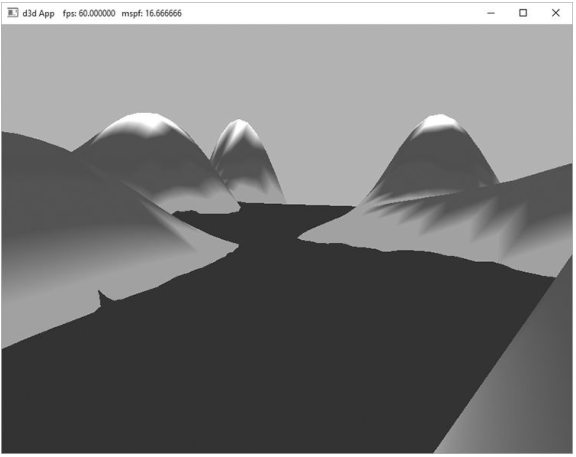
\includegraphics[width=\textwidth]{7-7}
    \centering
    \caption{“Lands and Waves”演示的屏幕截图。 因为我们还没有照明,所以很难看到波浪的形状。 按住“1”键可以在线框模式下查看场景,以更好地查看波形。}
    \label{fig:7-7}
\end{figure}

\begin{flushleft}
“漂亮”的实值(real-valued)函数$y=f(x,z)$的图是表面。 我们可以通过在$xz$平面中构建网格来近似表面,其中每个四边形由两个三角形构成,然后将函数应用于每个网格点; 见图\ref{fig:7-8}。
\end{flushleft}

\begin{figure}[h]
    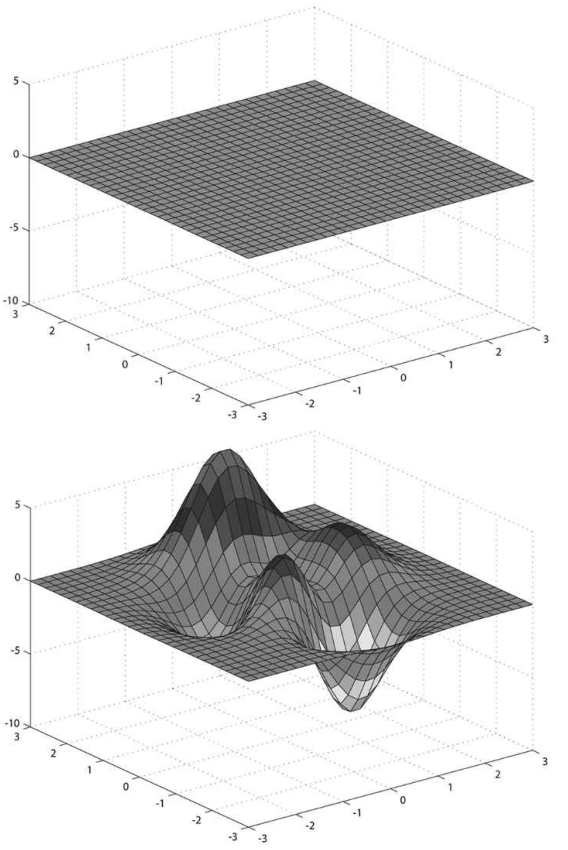
\includegraphics[width=\textwidth]{7-8}
    \centering
    \caption{(顶部)在xz平面中放置网格。(底部)对于每个网格点,应用函数f(x,z)以获得y坐标。 点(x,f(x,z),z)的图给出了曲面图。}
    \label{fig:7-8}
\end{figure}

%---- 7.7.1 ----
\subsection{创建网格顶点(Generating the Grid Vertices)}
\begin{flushleft}

\end{flushleft}



\end{document}
